\documentclass[twoside]{article}

%\usepackage{aistats2021}
% If your paper is accepted, change the options for the package
% aistats2021 as follows:
%
\usepackage[accepted]{aistats2021}
\usepackage{amsfonts}
\usepackage{graphicx}
\usepackage{multirow}
\usepackage{hyperref}
\usepackage{amsmath}
\usepackage{caption}
\usepackage{subcaption}
%
% This option will print headings for the title of your paper and
% headings for the authors names, plus a copyright note at the end of
% the first column of the first page.

% If you set papersize explicitly, activate the following three lines:
%\special{papersize = 8.5in, 11in}
%\setlength{\pdfpageheight}{11in}
%\setlength{\pdfpagewidth}{8.5in}

% If you use natbib package, activate the following three lines:
\usepackage{natbib}
%\renewcommand{\bibname}{References}
%\renewcommand{\bibsection}{\subsubsection*{\bibname}}

% If you use BibTeX in apalike style, activate the following line:
%\bibliographystyle{apalike}

\begin{document}

% If your paper is accepted and the title of your paper is very long,
% the style will print as headings an error message. Use the following
% command to supply a shorter title of your paper so that it can be
% used as headings.
%
%\runningtitle{I use this title instead because the last one was very long}

% If your paper is accepted and the number of authors is large, the
% style will print as headings an error message. Use the following
% command to supply a shorter version of the authors names so that
% they can be used as headings (for example, use only the surnames)
%
%\runningauthor{Surname 1, Surname 2, Surname 3, ...., Surname n}

\twocolumn[

\aistatstitle{TDHNN: Time-Dependent Hamiltonian Neural Networks }

\aistatsauthor{ Shaan A. Desai$^{1,2}$  \And  Marios Mattheakis$^{2}$ \And David Sondak$^{2}$ \And Pavlos Protopapas$^{2}$ \And Stephen Roberts$^{1}$ }

\aistatsaddress{ Machine Learning Research Group \\University of Oxford $^1$ \And School of Engineering and Applied Science \\ Harvard University $^2$ } ]


\bibliographystyle{abbrv}
\begin{abstract}

Learning the dynamics of complex physical systems requires models with well chosen inductive biases. Recently, it was shown that neural networks designed to learn a Hamiltonian and exploit Hamilton's equations significantly outperform existing approaches in predicting trajectories of autonomous systems that depend implicitly on time. Despite this success, many real world physical systems are non-autonomous and depend explicitly on time. In this paper, we address this challenge by embedding a modified Port-Hamiltonian into our neural networks that extends the general Hamiltonian to capture damped and forced systems alike. We show that our network can learn systems as complex as the duffing equation in the chaotic regime and recover the underlying Hamiltonian, force and damping terms. For such a system, we are also able to visually recover its Poincar\'e section - a crucial map in identifying chaotic trajectories.

%Unlike vanilla Artificial Neural Networks, Neural Networks embedded with physically-informed priors achieve remarkable results in accurately learning and predicting non-linear dynamical systems.
% despite this success, their generalization is often limited by the available training data which in practice only consists of a few short-range trajectories. naturally we might ask how we can generalize to unseen timesteps better?
% Despite this success, their generalization performance is often limited to short-range trajectories that run for less than the final training time. The performance degradation is due to state and energy drift induced by errors accumulating over time and it poses a critical challenge to learning highly non-linear and chaotic long-range dynamics precisely when data for only a limited number of short-range trajectories are available. One proposed solution to this challenge has been to incorporate symplectic integrators that aim to preserve the symplectic flow. Here, we present an alternative, an L1 penalty of the Hamiltonian derivative with respect to time: $d\mathcal{H}(p,q,t)/dt$. The inclusion of this term, a straightforward addition to the network, enforces the Hamiltonian to remain constant in time for a given trajectory. We empirically illustrate the stabilising effect this penalty has on our network. In addition, we use it solve problems in non-linear dynamics such as heinon-heiles, 3-body problem and double pendulum.
\end{abstract}

\begin{figure*}[ht!]
\centering
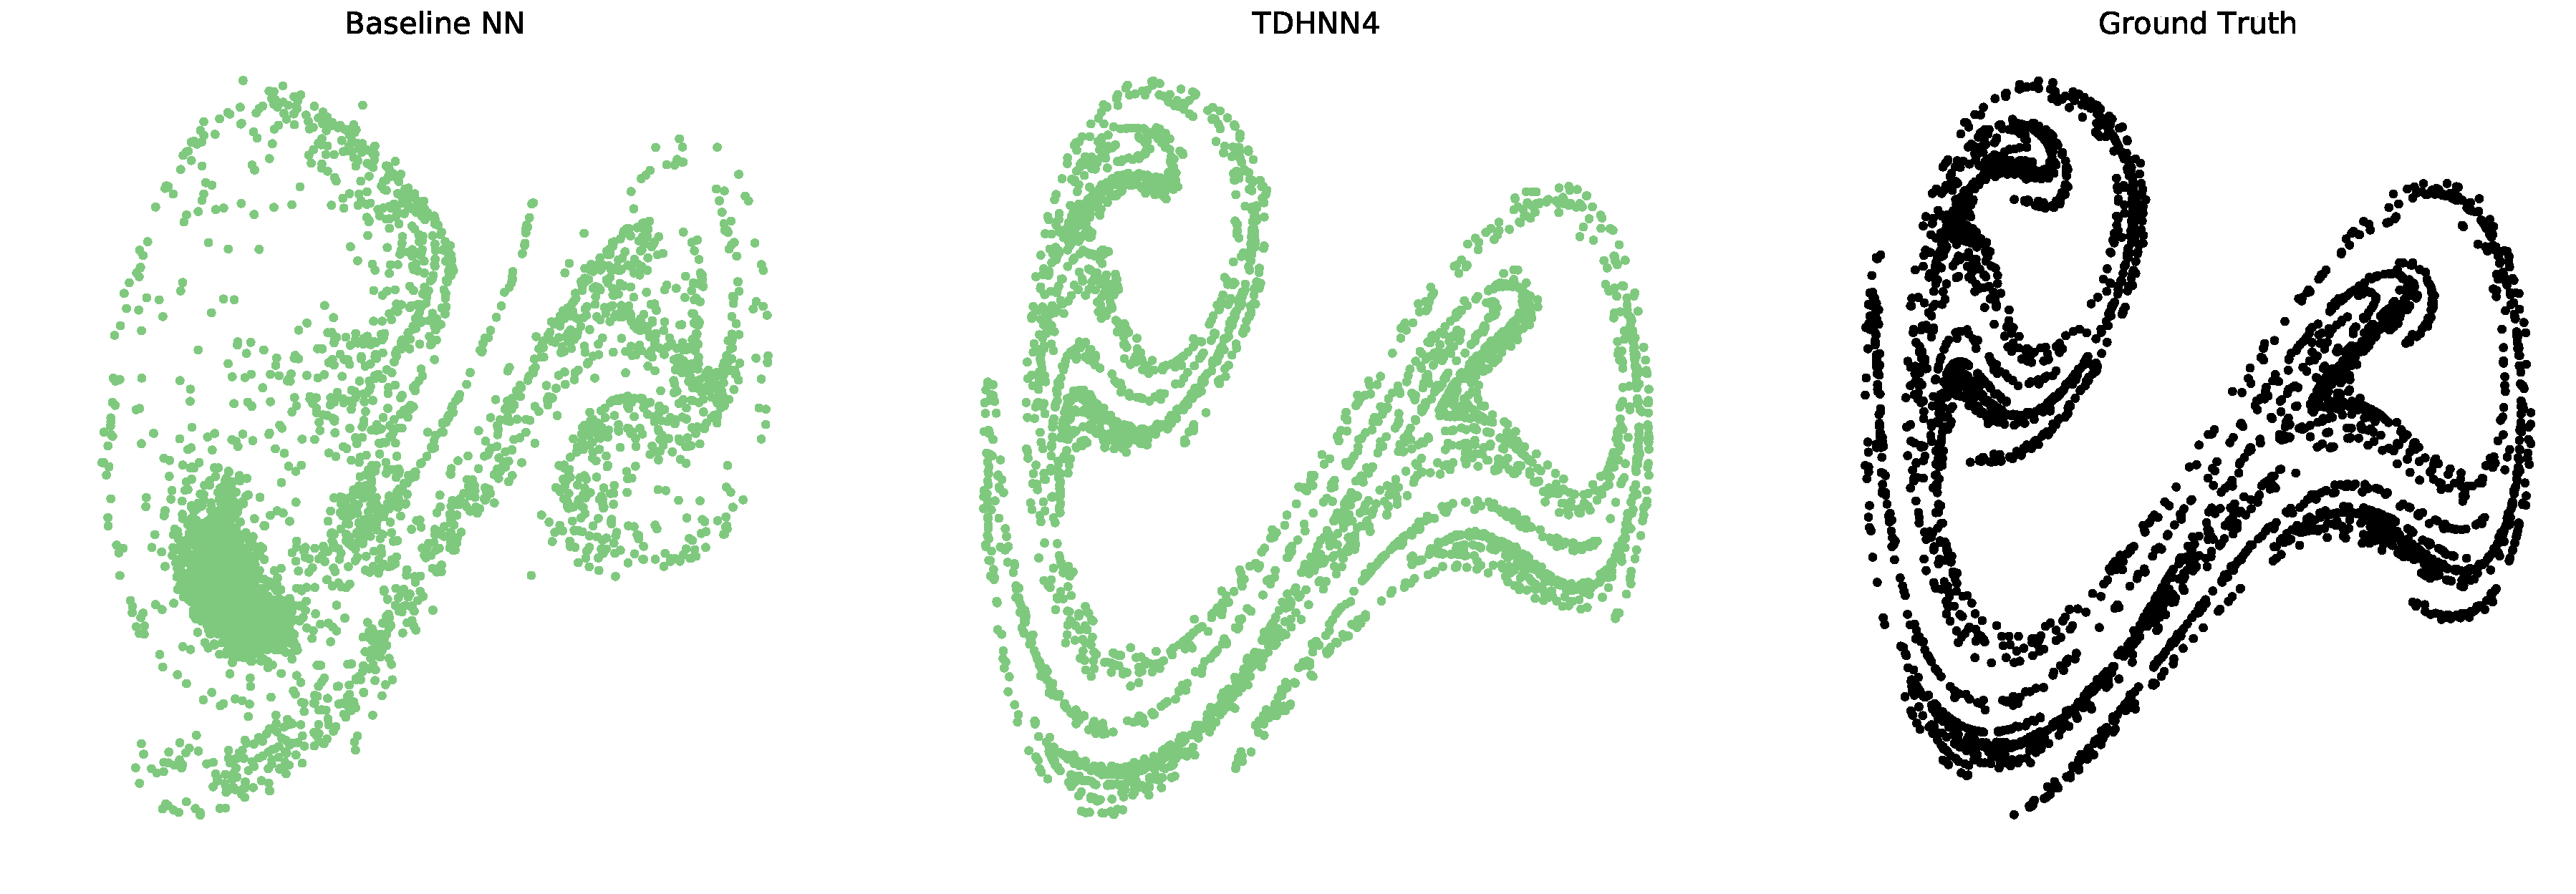
\includegraphics[width=0.9\textwidth]{figures/main_fig.pdf}
\caption{Poincar\'e Sections of a duffing oscillator in a chaotic regime. Both Baseline NN and TDHNN4 are trained for 20000 iterations with 2000 data points. TDHNN4 significantly outperforms Baseline NN at recovering the ground truth Poincar\'e section of a test point not in the training set.}
\label{fig.chaos1}
\end{figure*}

\section{Introduction}

Neural networks (NNs), as universal function approximators \cite{hornik_multilayer_1989}, have shown resounding success across a host of domains including image segmentation, machine translation and material property predictions. \cite{he_mask_2018,devlin_bert_2019,toussaint_differentiable_2018,yao_tensormol-01_2018}. However, their performance in learning physical systems has often been limited \cite{greydanus_hamiltonian_2019,pukrittayakamee_simultaneous_2009}. New research in \textit{scientific machine learning} - a field that tackles scientific problems with domain-specific machine learning methods, is paving a way to address these challenges. For example, it has been shown that physically informed inductive biases embedded in networks, such as Hamiltonian mechanics \cite{mattheakis_hamiltonian_2020, greydanus_hamiltonian_2019}, Lagrangians \cite{cranmer_lagrangian_2020, lutter_deep_2019}, Ordinary Differential Equations (ODEs) \cite{chen_neural_2018}, physics-informed networks \cite{raissi_physics_2017} and Graph Neural Networks \cite{battaglia_interaction_2016,sanchez-gonzalez_hamiltonian_2019} can significantly improve learning over vanilla neural networks in complex physical domains. Furthermore, it has also been shown that such systems can be adapted to learn trajectories of controlled dynamics \cite{lutter_deep_2019,zhong_dissipative_2020}. Despite this extensive research, there is no method that accounts for explicit-time dependence, a crucial component in forced dynamical systems. Additionally, many of the existing approaches do not outline how to account for energy dissipation. Inspired by \cite{zhong_dissipative_2020}, we show that by embedding a Port-Hamiltonian into a neural network we can learn the dynamics of explicit time-dependent physical systems. We benchmark our network on a range of tasks from the simple mass-spring system to a chaotic duffing equation for a relativistic particle. Our network consistently outperforms other approaches while actively learning both the driving force and damping coefficient. 

\section{Background}

\subsection{Hamiltonian Neural Networks}

Recently, the authors of \cite{greydanus_hamiltonian_2019} demonstrate that the dynamics of an energy conserving autonomous system can be accurately learned by guiding a neural network to predict a Hamiltonian - an important representation of a dynamical system that generalizes classical mechanics. The Hamiltonian $\mathcal{H}$ is a scalar function of a position vector $\mathbf{q} = (q_1,q_2,....,q_M)$ and momentum vector $\mathbf{p} = (p_1,p_2,....,p_M)$ of a given system that obeys Hamilton's equations eqn.\ref{eqn.hamiltonian}.
\begin{equation}
\dot{\mathbf{q}}= \frac{\partial \mathcal{H}}{\partial \mathbf{p}}, ~~~
\dot{\mathbf{p}}= -\frac{\partial \mathcal{H}}{\partial \mathbf{q}}
\label{eqn.hamiltonian}
\end{equation}

As such, it is noted in \cite{greydanus_hamiltonian_2019} that by parametrizing the Hamiltonian with a neural network e.g. $H_{\theta}(\mathbf{q},\mathbf{p})$ where $\theta$ represents the parameters of a deep neural network and $\mathbf{q},\mathbf{p}$ are the inputs to the network, one can easily obtain the system's dynamics by differentiating (via autograd) the Hamiltonian with its inputs. In other words, the derivatives of the Hamiltonian with respect to the input $\left [ \frac{\partial \mathcal{H}}{\partial \mathbf{p}},-\frac{\partial \mathcal{H}}{\partial \mathbf{q}} \right ]$ provide us with time derivatives of the input state vector $[\dot{\mathbf{q}},\dot{\mathbf{p}}]$. Once trained, this network therefore yields an approximate time derivative generator for the state $[\mathbf{q},\mathbf{p}]$ and as such can be used in a numerical integrator to evolve an initial condition $[\mathbf{q}_t,\mathbf{p}_t]$ as in \ref{eqn.action_int}.
\begin{equation}
(\mathbf{q},\mathbf{p})_{t+1} = (\mathbf{q},\mathbf{p})_t + \int_t^{t+1} \left [ \frac{\partial \mathcal{H}}{\partial \mathbf{p}},-\frac{\partial \mathcal{H}}{\partial \mathbf{q}} \right ] \mathrm{d}t
\label{eqn.action_int}
\end{equation}
In addition, the vector field $\mathbf{S} = \left [ \frac{\partial \mathcal{H}}{\partial \mathbf{p}},-\frac{\partial \mathcal{H}}{\partial \mathbf{q}} \right ]$ is a symplectic gradient. This means that $\mathcal{H}$ remains constant as long as the state vectors are integrated along $\mathbf{S}$. This result links the Hamiltonian with the total energy of the system such that $\mathcal{H}(\mathbf{q},\mathbf{p}) = E_{tot}$ for many autonomous physical systems. Therefore, the Hamiltonian is a powerful inductive bias that can be utilised to evolve a physical state while maintaining energy conservation. However, this formulation does not readily generalize to damped or forced system.

\subsection{Port-Hamiltonians}

The Port-Hamiltonian is a formalism that allows us to generalize Hamilton's equations to incorporate damping and forcing terms. The first method to embed the Port-Hamiltonian in a neural network \cite{zhong_dissipative_2020} shows how to represent a general form for such a system. In \cite{zhong_dissipative_2020} the Port-Hamiltonian is represented as:
\begin{equation}
\resizebox{0.9\linewidth}{!}{$%
\begin{bmatrix}
\dot{\mathbf{q}} \\
\dot{\mathbf{p}}
\end{bmatrix}
=
\Bigg(\begin{bmatrix}
0 & \mathbf{I} \\
-\mathbf{I} & 0
\end{bmatrix} +
\mathbf{D}(\mathbf{q})
 \Bigg)
 \begin{bmatrix}
\frac{\partial \mathcal{H}}{\partial \mathbf{q}} \\
\frac{\partial \mathcal{H}}{\partial \mathbf{p}}
\end{bmatrix}
+
\begin{bmatrix}
0 \\
\mathbf{g}(\mathbf{q})
\end{bmatrix}
u
$%
}%
\label{eqn.pham}
\end{equation}
where $\mathbf{D}(\mathbf{q})$ is a matrix to account for damping and $g(q)u$ is an external constant control term. 

This general formalism allows us to collapse to a classical Hamiltonian system by simply setting $\mathbf{D}$ and $u$ to zero. Note here that the authors of \cite{zhong_dissipative_2020} assume the vector $[\mathbf{q},\mathbf{p},u]$ is provided as input to the system. The matrix $\mathbf{D}(\mathbf{q})$ is assumed to be semi-positive definite and $g(\mathbf{q})$ is typically a non-linear scaling of $\mathbf{q}$.

\section{Related Work}

Numerous recent methods highlight how to connect physically-informed inductive biases with neural networks.

\subsection*{Functional Priors}
Functional priors, for example, embed the full functional form of an equation into the neural network. Physics-informed Neural Networks (PINNs) \cite{raissi_physics_2017,raissi_physics-informed_2019} and Hamiltonian Nets \cite{mattheakis_hamiltonian_2020} look at directly embedding the equations of motion into the loss function. While PINNs is a data-driven approach that relies on autograd to compute partial-derivatives of a hidden state, Hamiltonian Nets is a data-independent approach that pre-specifies the full equation form in the loss function.

\subsection*{Integrator Priors}
Many recent methods seek to use a NN to parametrize the time derivatives of a state vector and then use this learned parametrization in a scientific integrator such as a Runge-Kutta method. The authors of NeuralODE \cite{chen_neural_2018} show that embedding the integrator into the learning process induces a continuous depth neural network for large time-step predictions. As such, the number of gradient computations scales exponentially with the number of integrative time steps. The paper re-introduces the adjoint method to ensure linear scaling of the gradient computations. Other work such as \cite{zhu_deep_2020} shows the need for symplectic integrators 

\subsection*{Graph based methods}
In \cite{battaglia_interaction_2016}, the authors show how a Graph Neural Network, designed to capture the relational structure of systems, can be used to learn interacting particle systems. This work has been exploited in numerous advances \cite{sanchez-gonzalez_graph_2018,sanchez-gonzalez_learning_2020,cranmer_lagrangian_2020}.

\subsection*{Lagrangian/Hamiltonian Methods}
While \cite{cranmer_lagrangian_2020} and \cite{greydanus_hamiltonian_2019} propose to explicitly learn Hamiltonian and Lagrangian functions, \cite{lutter_deep_2019} shows how one can exploit the Lagrangian equation to learn both a function which can predict the generalized forces as well as use generalized forces and coordinate information to predict the next state. The authors show that their inverse model can accurately predict a controlled double pendulum, which is pertinent for controlled robots.


\subsection*{Latest Advances}
Constrained HNN \cite{finzi_generalizing_2020}, one of the most recent advances published as a spotlight in NeurIPS 2020, looks at enforcing cartesian coordinates in Hamiltonians and Lagrangians with holonomic constraints. The paper emphasises that such a framework works significantly better at learning deeply complex physical systems such as the 5-pendulum. 


\section{Method}

\subsection*{Theory}
Our method, TDHNN4, takes the form of the Port-Hamiltonian described earlier with two modifications. First, our approach exploits the fact that most damped systems consist of a non-zero, state-independent term in the lower right quadrant, so we replace the damping matrix $\mathbf{D}(\mathbf{q})$ with a single parameter independent of $\mathbf{q}$ in the lower right half of the matrix. Secondly, in order to generalize to time dependent forcing, we replace $g(\mathbf{q})u$ with $F(t)$. The resulting representation, as highlighted in eqn.\ref{eqn.pham1}, is now general enough to handle many well-known forced systems but also specific enough to tackle learning in complex physical domains.

\begin{equation}
\resizebox{0.9\linewidth}{!}{$%
\begin{bmatrix}
\dot{\mathbf{q}} \\
\dot{\mathbf{p}}
\end{bmatrix}
=
\Bigg(\begin{bmatrix}
0 & \mathbf{I} \\
-\mathbf{I} & 0
\end{bmatrix} +
\begin{bmatrix}
0 & 0 \\
0 & \mathbf{D}
\end{bmatrix}
 \Bigg)
 \begin{bmatrix}
\frac{\partial \mathcal{H}}{\partial \mathbf{q}} \\
\frac{\partial \mathcal{H}}{\partial \mathbf{p}}
\end{bmatrix}
+
\begin{bmatrix}
0 \\
\mathbf{F}(t)
\end{bmatrix}
$%
}%
\label{eqn.pham1}
\end{equation}
\begin{figure}[h!]
\centering
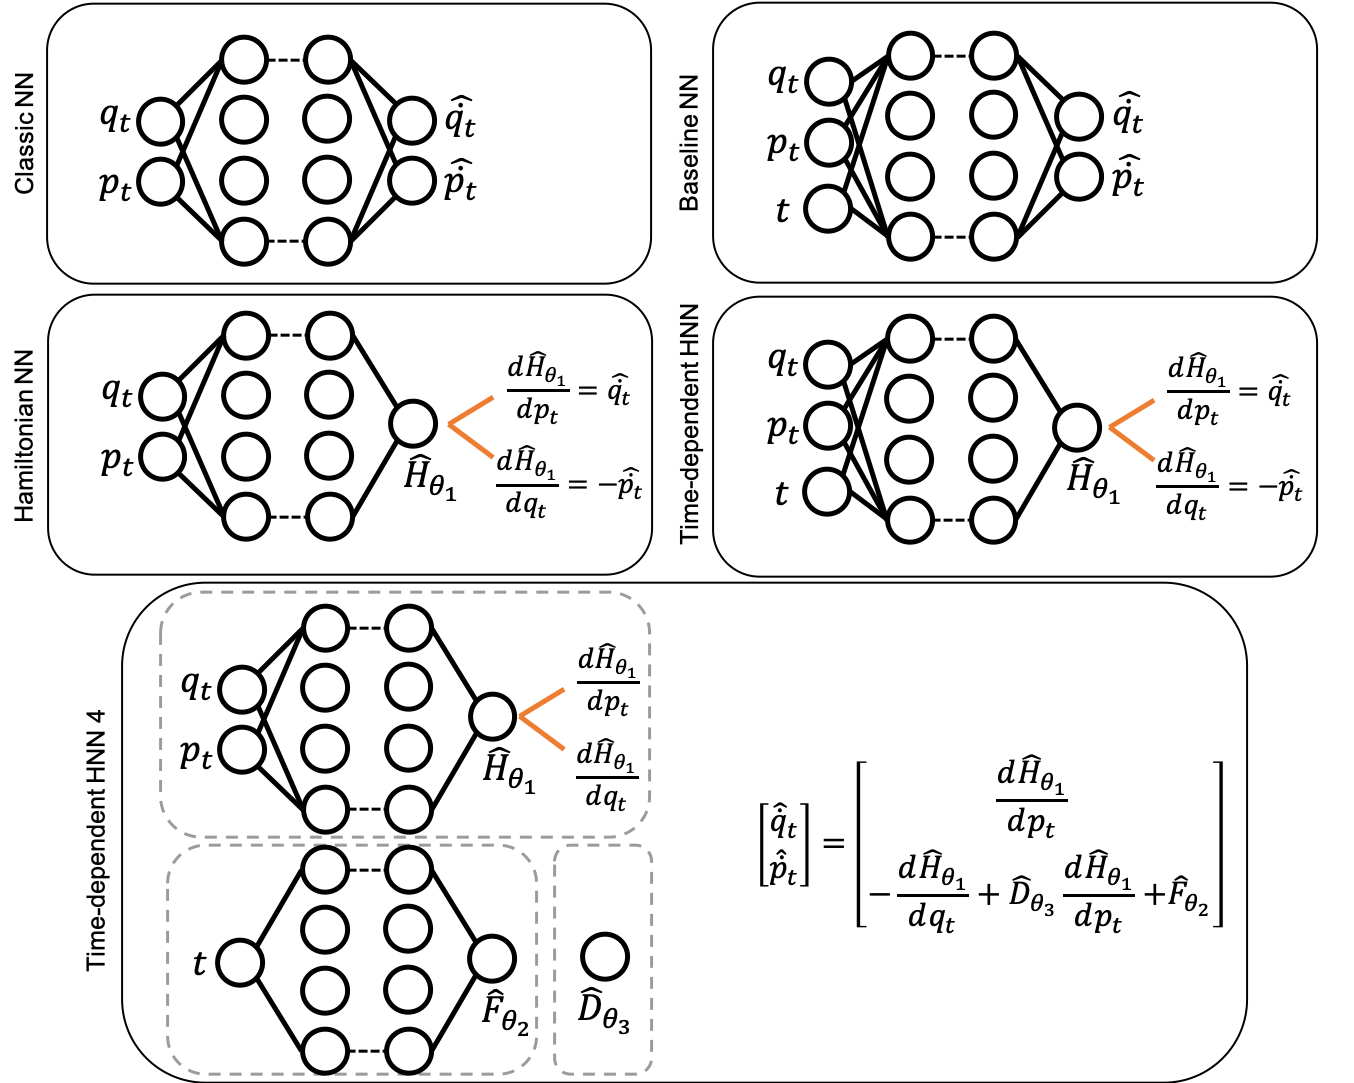
\includegraphics[width=0.5\textwidth]{figures/architect.png}
\caption{Architectures used to learn dynamics in this paper. The naive extension of classic NN and Hamiltonian NN (top left) is to incorporate time as an additional input variable (top right). Our innovation, which exploits Port-Hamiltonians, explicitly learns the force $F_{\theta_2}$ as well as the damping coefficient $D_{\theta_3}$.}
\label{fig.architecture}
\end{figure}

The architecture for our method can be seen in figure \ref{fig.architecture}. We embed the port-hamiltonian by learning 3 main components: the Hamiltonian $H$, the driving force $F$ and the damping term $D$ each parametrized by a neural network.
%We define the loss function for our architecture as follows:
%\begin{multline}
%\mathcal{L} =\left\| \frac{\partial \mathbf{p}}{\partial t} +\frac{\partial \mathcal{H}_{\theta_1}}{\partial \mathbf{q}} -\mathbf{D}_{\theta_3}\frac{\partial \mathcal{H}_{\theta_1}}{\partial \mathbf{p}} - \mathbf{F}_{\theta_2}(t) \right\|_2^2 +
%\\
%\left\|\frac{\partial \mathbf{q}}{\partial t} - \frac{\partial \mathcal{H}_{\theta_1}}{\partial \mathbf{p}} \right\|_2^2+ \alpha_{reg}|| \mathbf{F}_{\theta_2} (t)||_1 + \beta_{reg}||\mathbf{D}_{\theta_3}||_1 
%\end{multline}
\subsection*{Training}
To train the network, we feed in a state-vector $ [\mathbf{q},\mathbf{p},\mathbf{t}]$ to our model. The first component $\mathcal{H}_{\theta_1}$ consists of 3 hidden layers designed to predict $\mathcal{H}$ from $[\mathbf{q},\mathbf{p}]$ input data. The second component $\mathbf{D}_{\theta_3}$ consists of a single weight parameter (i.e. $\theta_3$ is a single node) designed to learn the damping $\mathbf{D}$ and the third neural-network consists of 3 hidden layers designed to predict $\mathbf{F}(t)$. The output of each component is combined as in the equation in fig.\ref{fig.architecture} to obtain predictions of the state time derivatives $[\hat{\dot{\mathbf{q}}},\hat{\dot{\mathbf{p}}}]$. Note that the Hamiltonian learned is a single value for each input that is differentiated (via autograd) with respect to the input $[\mathbf{q},\mathbf{p}]$ to obtain components of the predicted time derivative. We can think of these as being the state time derivatives in the unforced and undamped setting. Using these predictions, we define our loss function as:
\begin{equation}
\mathcal{L} =|| \hat{\dot{\mathbf{q}}}_t - \mathbf{\dot{q}}_t ||_2^2 +
|| \hat{\dot{\mathbf{p}}}_t -\mathbf{\dot{p}}_t ||_2^2 + \alpha|| \mathbf{F}_{\theta_2} (t)||_1 + \beta||\mathbf{D}_{\theta_3}||_1 
\label{eqn.loss}
\end{equation}
We use an L2-norm penalty for the predicted state-vectors and an L1-norm for force and damping to encourage sparsity. We introduce the sparsity-inducing L1-norm on force and damping because we want our network to identify both classical autonomous systems (which may not have force or time-varying components) as well as non-autonomous systems. The choice of hyperparameters $\alpha$ and $\beta$ is made via a grid search across $[10^{-2},10^{-4},10^{-6},10^{-8}]$, for each parameter, that generates the lowest validation loss (details in Appendix D). For our experiments we use 200 nodes per layer and find that most activations, including tanh, sin and cos yield comparable results. To benchmark our method, we use a modified classic neural network that takes in an additional time vector and predicts $[\dot{\mathbf{q}},\dot{\mathbf{p}}]$. We also take the straightforward extension of HNN to include time as variable input. 

\subsection*{Testing}
Once trained, each of the networks in figure  \ref{fig.architecture} can approximate $[\dot{\mathbf{q}},\dot{\mathbf{p}}]$. As such, they can be used in a scientific integrator such as a Runge-Kutta 4th order method to integrate initial conditions from $t=0$ to $t=T_{max}$ which we refer to as a state rollout. We measure the performance of the network by comparing the predicted state rollout with the ground truth (measured using a scientific integrator and the ground truth time derivatives). We do this by computing a mean squared error across the state variables and across time. Therefore:

\begin{equation}
MSE_{state} = \frac{1}{2N} (\sum_{i=1}^N (\mathbf{q}_i-\hat{\mathbf{q}}_i)^2 + \sum_{i=1}^N (\mathbf{p}_i - \hat{\mathbf{p}}_i)^2)
\end{equation}

\begin{equation}
MSE_{energy} = \frac{1}{N} \sum_{i=1}^N (\mathcal{H}(\mathbf{q}_i,\mathbf{p}_i)-\mathcal{H}(\hat{\mathbf{q}}_i,\hat{\mathbf{p}}_i))^2
\end{equation}

where $N = T_{max}/\Delta t $. We typically compute these terms for multiple different initial conditions during inference and average across them (see Fig. \ref{mspring} c).



\subsection*{Procedure}

\begin{enumerate}
\item collect state variable data $[\mathbf{q},\mathbf{p},t]$ and time derivatives $[\dot{\mathbf{q}},\dot{\mathbf{p}}]$ from trajectories of a given system.
\item Feed state-variable information into TDHNN4 which will learn a Hamiltonian, force and damping term to predict $[\hat{\dot{\mathbf{q}}},\hat{\dot{\mathbf{p}}}]$.
\item minimize predictions with ground truth time-derivatives as in equation \ref{eqn.loss}.
\item Once trained, use the network as a time-derivative generator in a scientific integrator to integrate a set of initial conditions $[q_0,p_0]$ to $[q_T,p_T]$.
\end{enumerate}


\section{Results}

We benchmark the performance of our models on numerous datasets that canvas time-independent systems to complex chaotic forced systems. 

\subsection{Simple Mass Spring}

We begin our analysis with a simple mass spring system which is a well known system from classical physics that obeys Hooke's Law. The Hamiltonian for a simple mass spring system is written as:
\begin{equation}
\mathcal{H} = \frac{1}{2}kq^2 + \frac{1}{2m}p^2 
\end{equation}
where $k$ is the spring constant and $m$ is the mass of the block. 

\textbf{Training:} Without loss of generalization, we set $k$ and $m$ to 1 for our experiments. We sample 25 initial training conditions $[q_0,p_0]$ that satisfy $q_0^2+p_0^2 = r_0^2$ where $1 \leq r_0 \leq 4.5$ similar to \cite{greydanus_hamiltonian_2019} and integrate each using a 4th order RK method with $\Delta t =0.05$ and $T_{max} = 3.05$. In other words, the initial conditions are sampled in a disc with radii between 1 and 4.5.

\textbf{Test:} At test time, we sample 25 initial conditions not in the training set and evolve them to $T_{max}=6.1$. The test error in fig.\ref{mspring} is measured as the Mean Squared Error (MSE) between the ground truth and predicted state and energy values for a given trajectory. We also show the average state and energy MSE across 25 trajectories. 

We investigate this simple system to show that learning a separate, regularised forcing term results in much better state and energy predictions in comparison to TDHNN and baseline NN. The main reason for this is that while TDHNN and baseline NN learn dynamics with time-steps within the training regime, they typically cannot generalize to unseen time-steps. Learning a separate forcing term and regularizing it keeps the time component independent of the Hamiltonian and therefore allows us to closely match the performance of classical time-implicit HNN.

\begin{figure}[h!]
\centering
%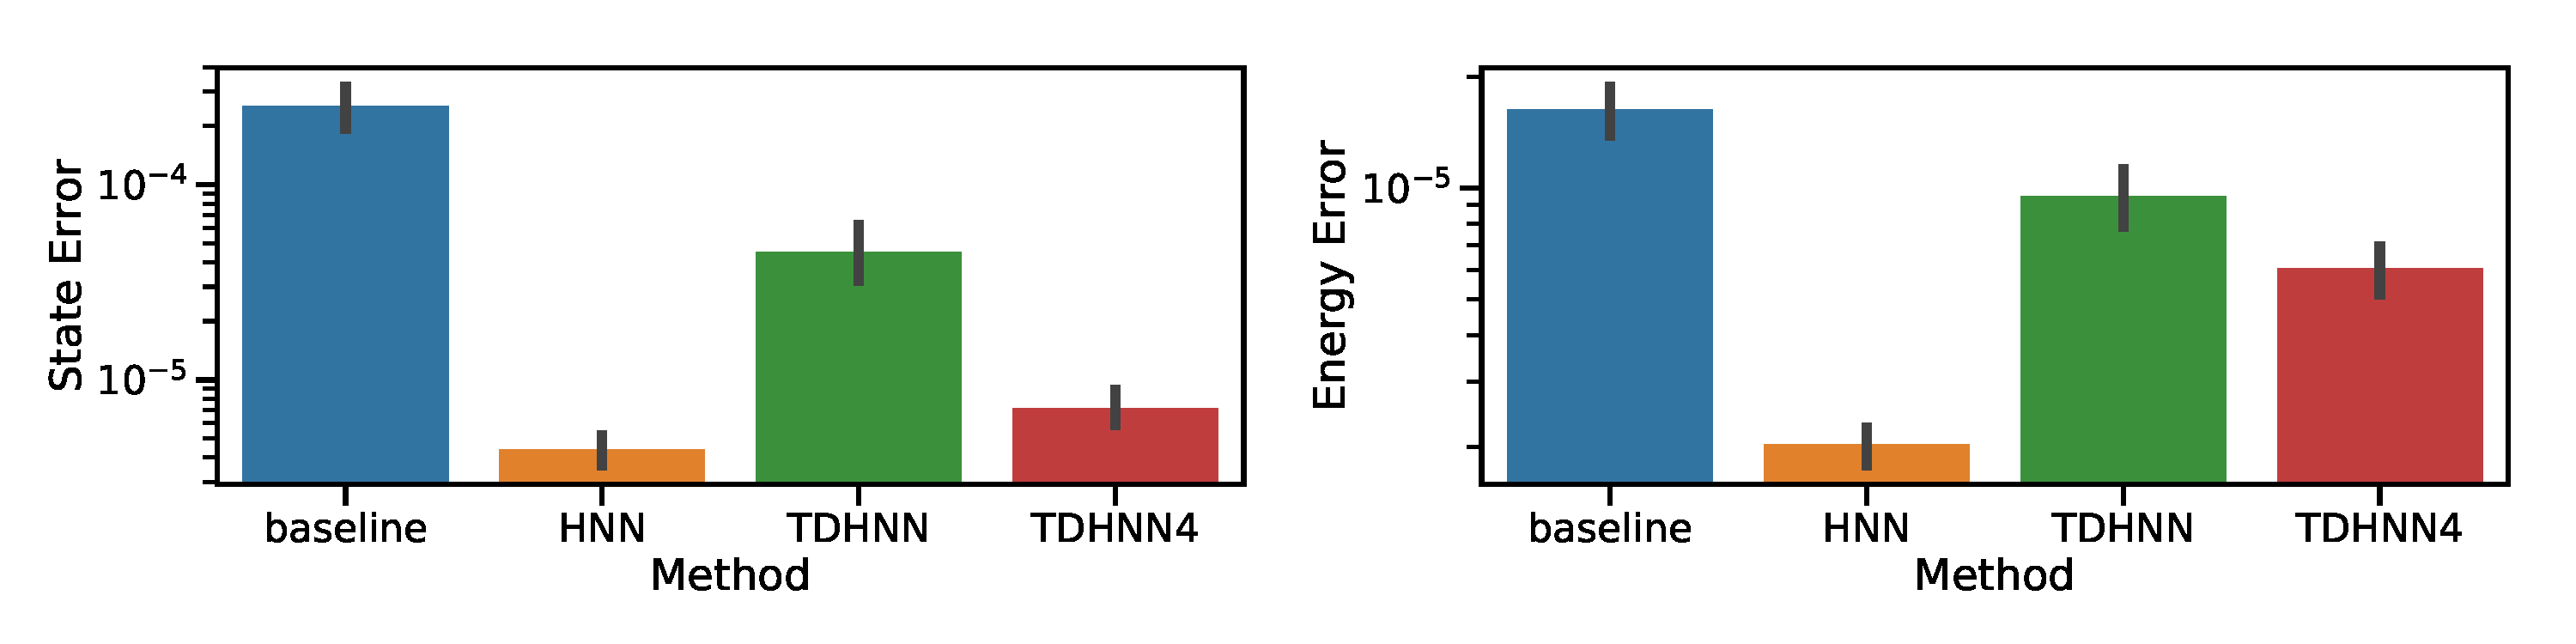
\includegraphics[width=0.4\textwidth]{figures/mass_spring_errors.pdf}
\captionsetup{justification=centering}
	\begin{subfigure}[b]{0.4\textwidth}
		\centering
		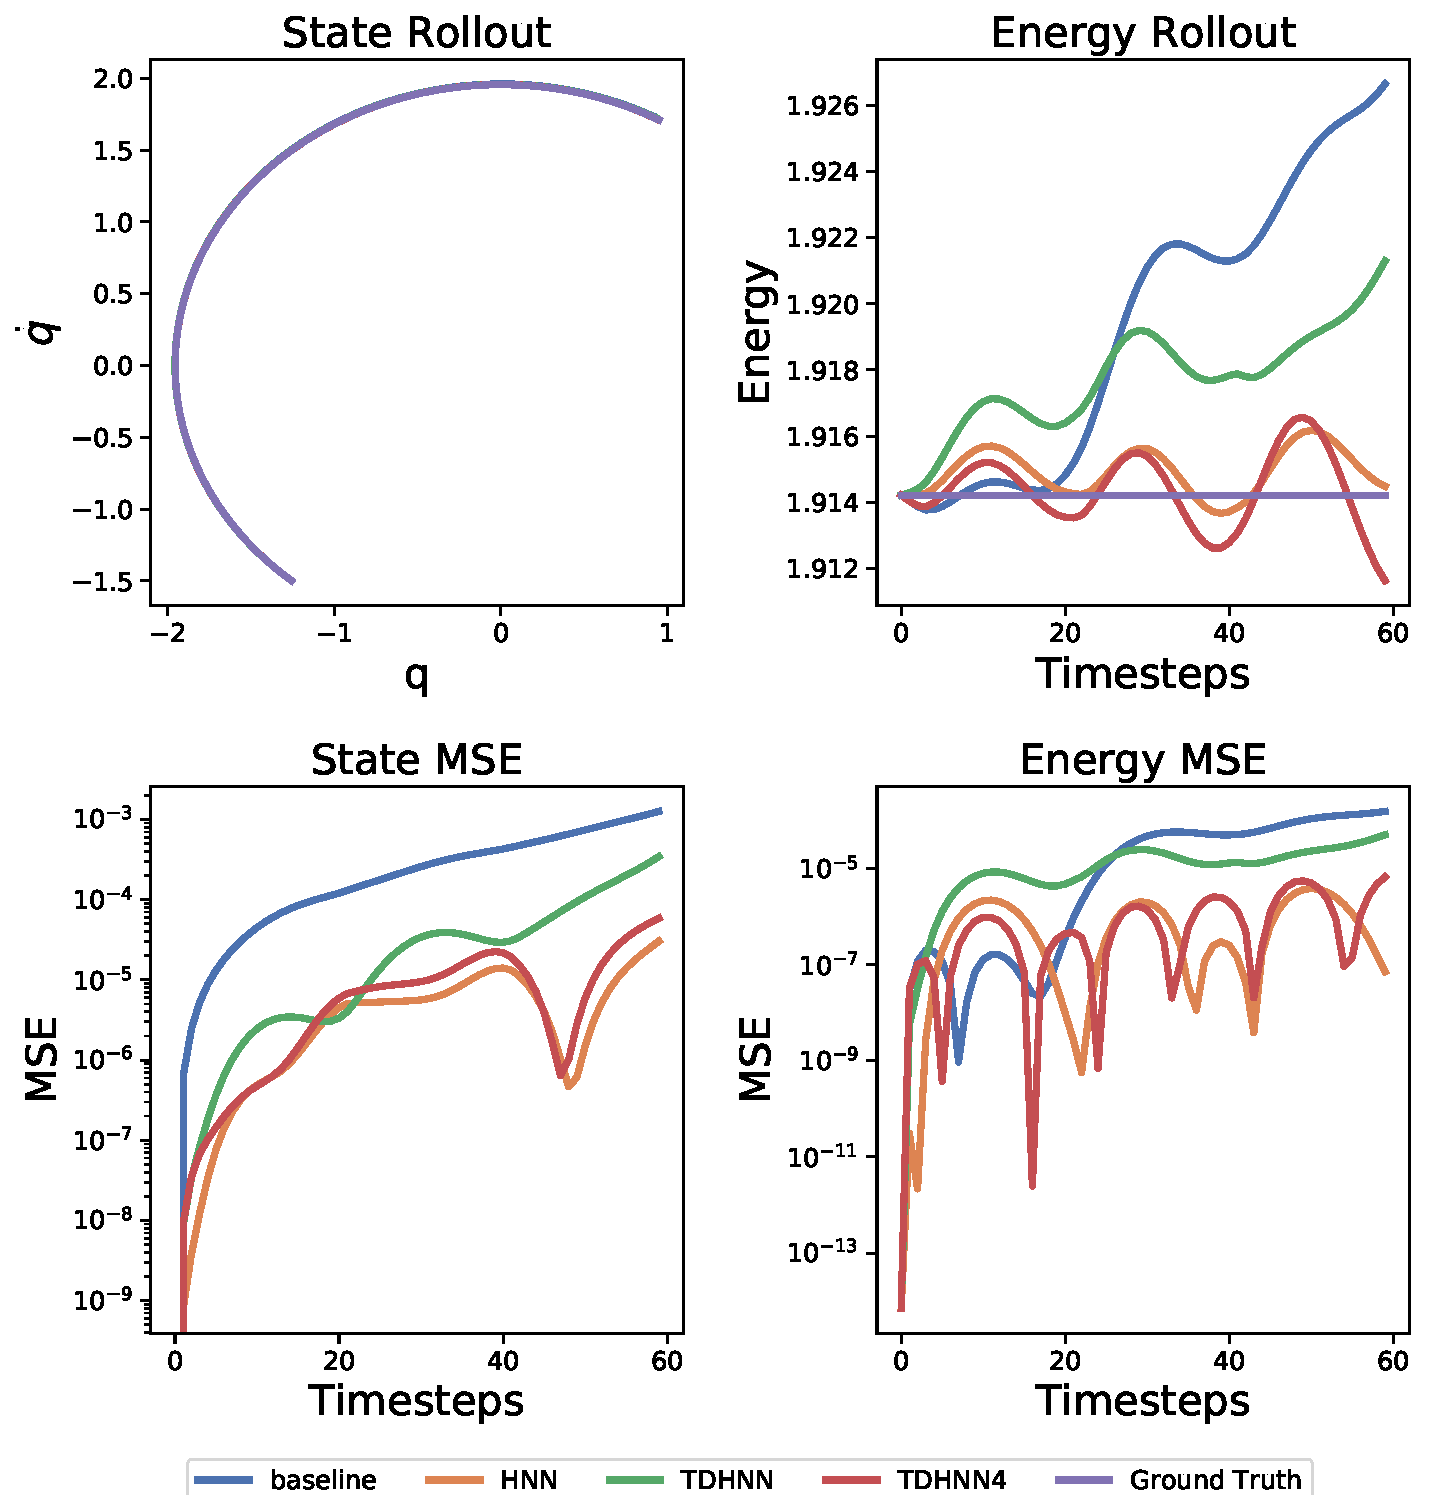
\includegraphics[width=\textwidth]{figures/figures/mass_spring/1/mass_spring_long_0.pdf}
		\caption{State and energy rollout/MSE of an initial condition in the test set.}
	\end{subfigure}
	\begin{subfigure}[b]{0.48\textwidth}
		\centering
		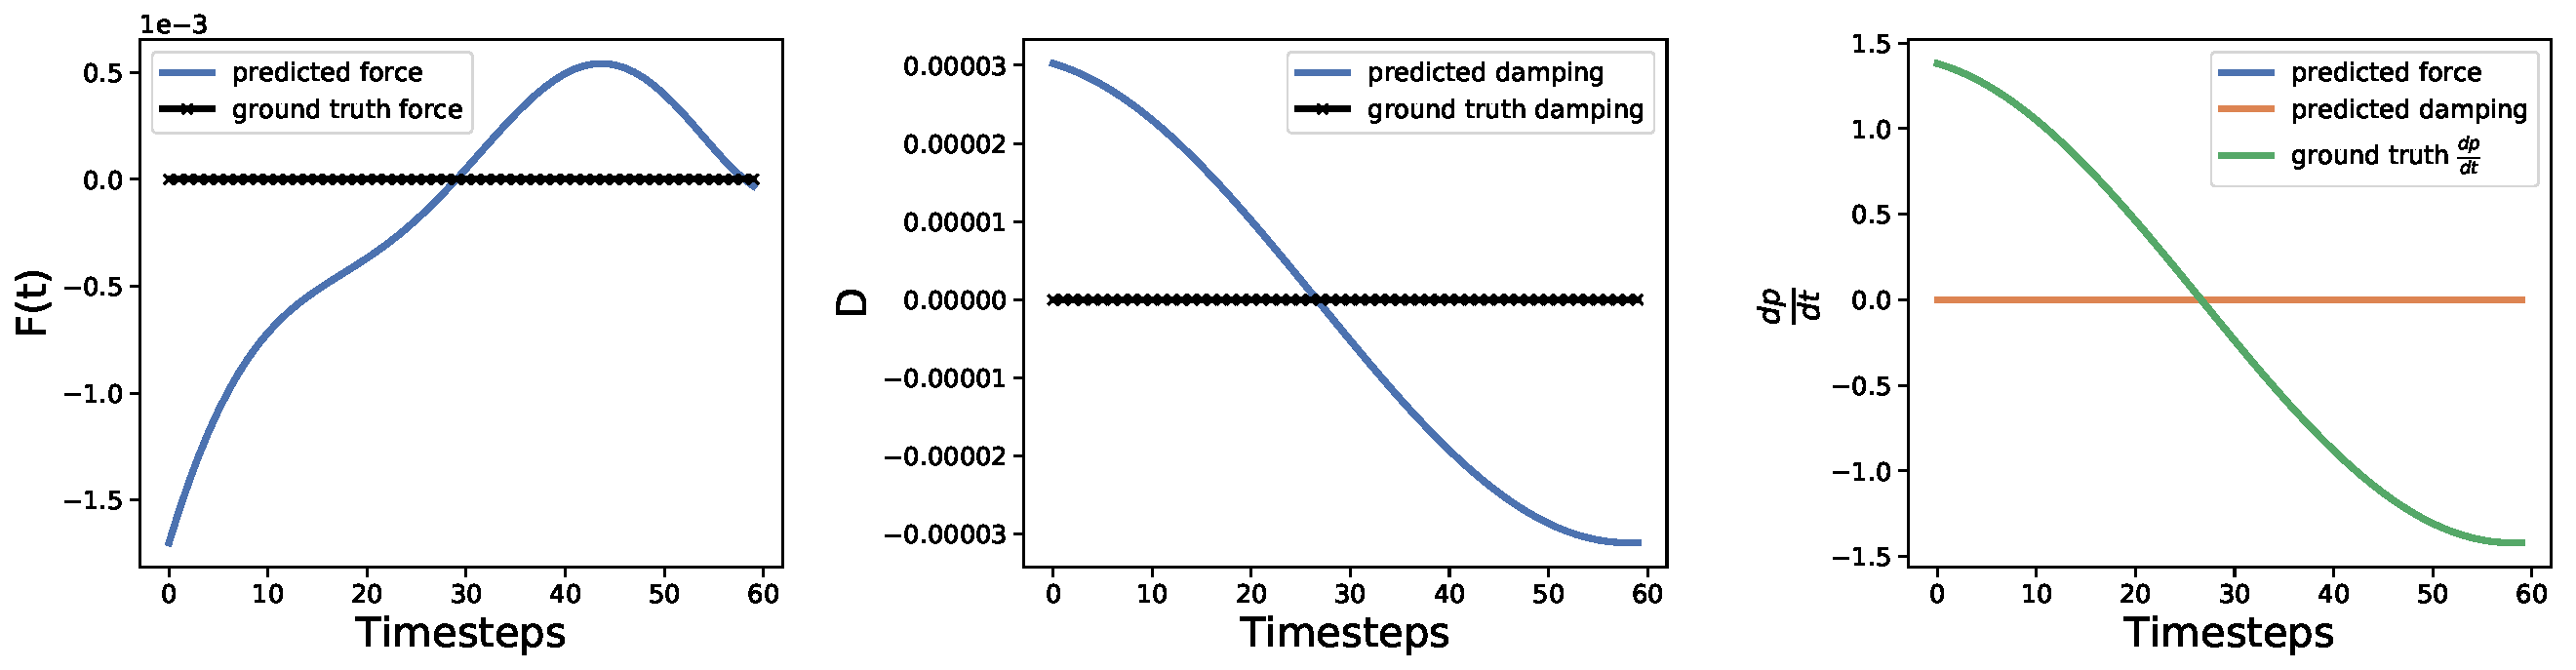
\includegraphics[width=\textwidth]{figures/figures/mass_spring/1/mass_spring_dpdt_0.pdf}
		\caption{Learnt force and damping terms and their contribution to $dp/dt$}
	\end{subfigure}
	\begin{subfigure}[b]{0.48\textwidth}
	    \centering
		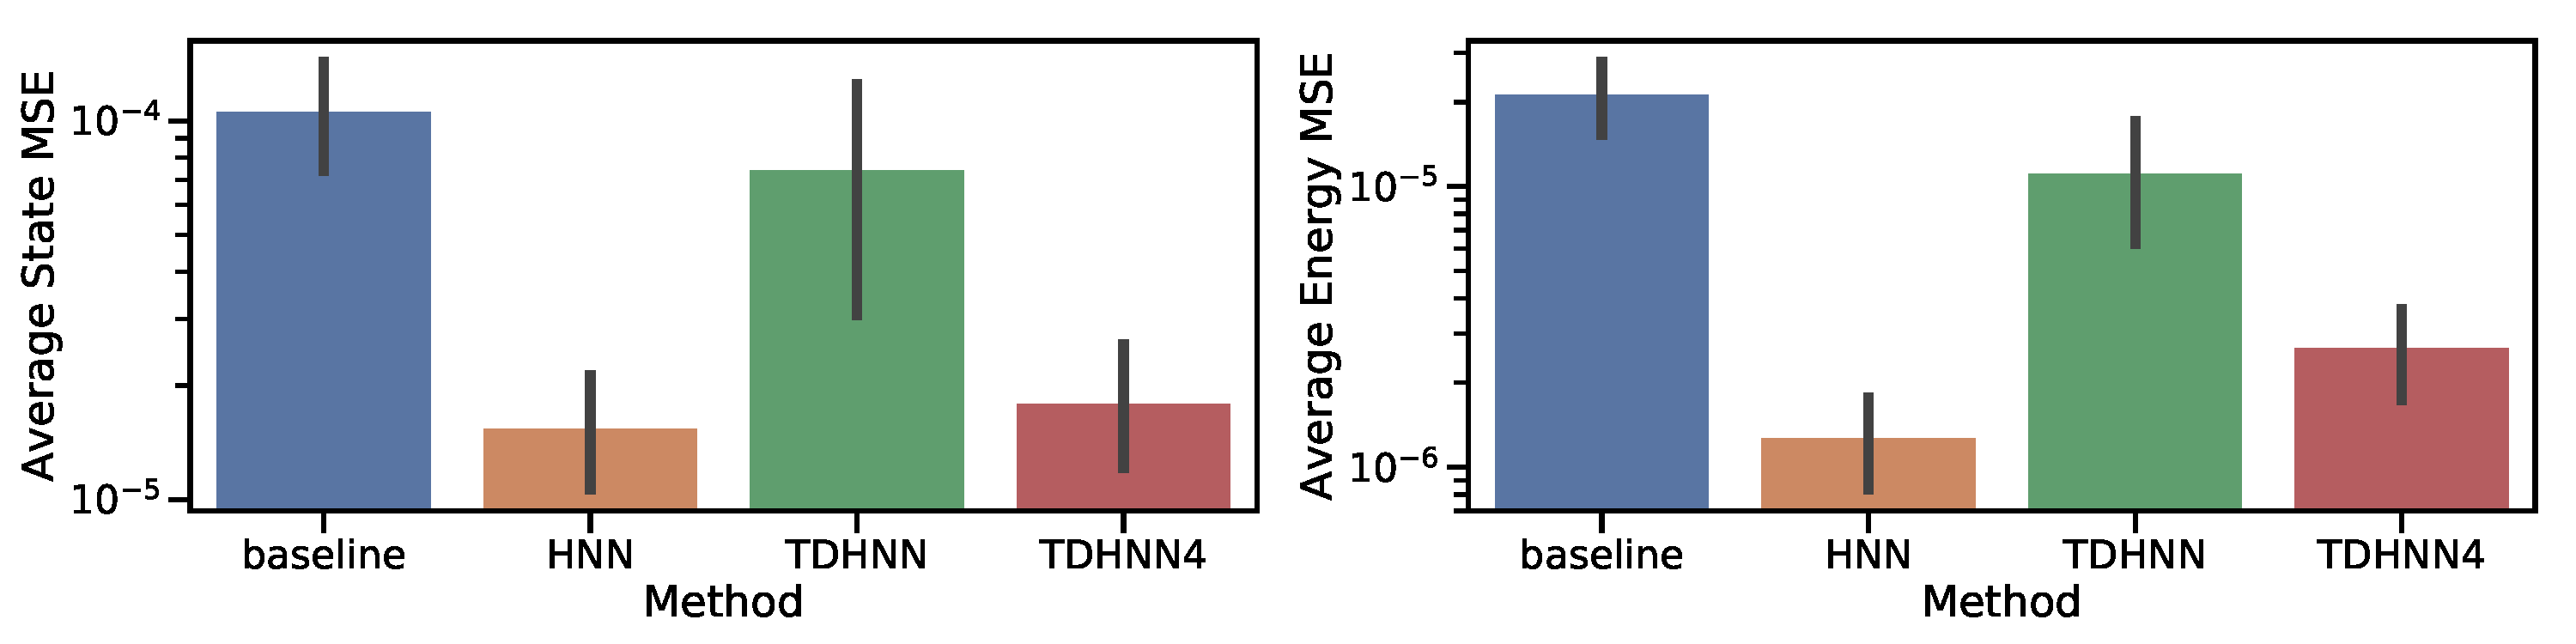
\includegraphics[width=\textwidth]{figures/figures/mass_spring/1/mass_spring_errors_0.pdf}
		\caption{Rollout state and energy MSE averaged across 25 initial test states}
	\end{subfigure}
\caption{The simple mass spring system has no explicit time dependence. We see that TDHNN4 can almost recover the dynamics as well as HNN. Baseline and TDHNN are unable to achieve the same test state error as they are only reliable for time steps that are within the training regime.}
\label{mspring}
\end{figure}


\subsection{Damped Mass Spring}

We extend the simple mass spring system to include a damping term that reduces the initial energy of the system over time. Of course the inclusion of this term violates energy conservation and therefore we cannot write a Hamiltonian for such a system (see Appendix A.1 for details). 

However, as we saw with Port-Hamiltonians, there is a straightforward way to account for the damping term without explicitly defining a full Hamiltonian. By combining a regular Hamiltonian $\mathcal{H}_{reg}$ with an additional term that learns the damping, we can disentangle the two terms for learning. Indeed, there are alternative methods to do this, including generalised Hamiltonian decomposition which we do not explore here.

\textbf{Training:} We have 20 initial training conditions, with position and momentum uniformly sampled in $[-1,1]^2$. Each trajectory is evolved until $T_{max} = 30.1$ with a $\Delta t = 0.1$. We fix the damping coefficient $\delta = 0.3$.

\textbf{Test:} At inference, we compute the average rollout MSE of 25 unseen initial conditions sampled and evaluated the same way as training, and report the average state and energy rollout MSE for initial conditions that are not in the training set (see Fig.\ref{damped}).



\begin{figure}[h!]
\centering
\captionsetup{justification=centering}
%	\begin{subfigure}[b]{0.4\textwidth}
%		\centering
%		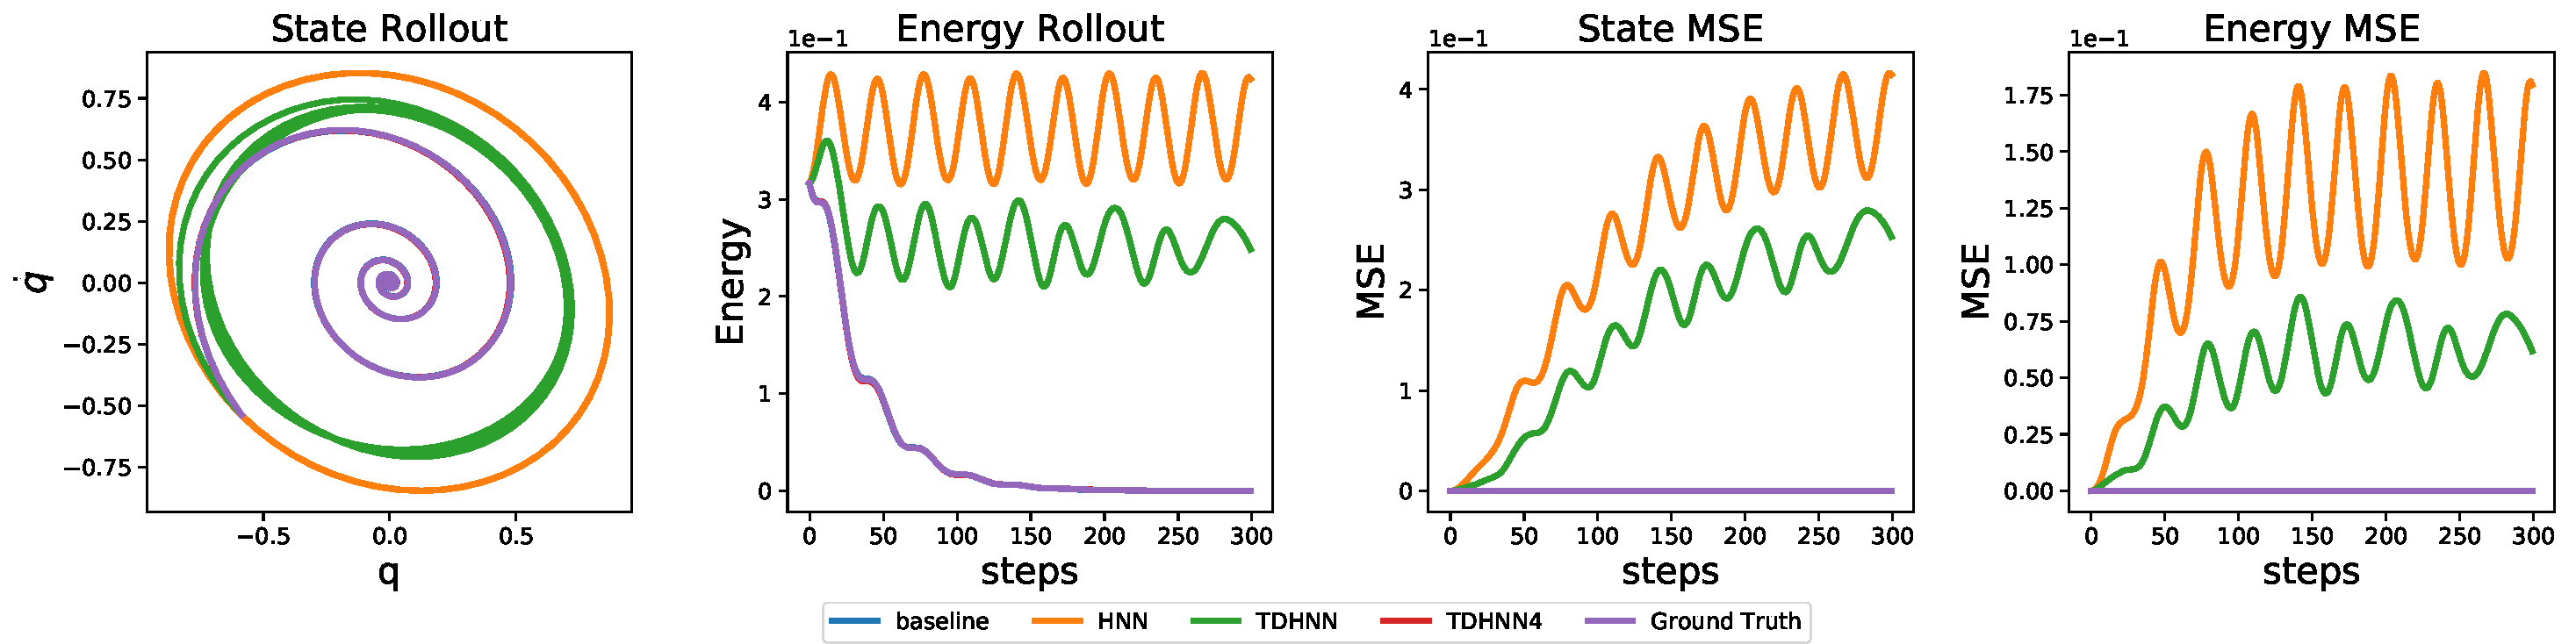
\includegraphics[width=\textwidth]{figures/damped_1_pred.pdf}
%		\caption{State and energy rollout/MSE of an initial condition in the test set.}
%	\end{subfigure}
	\begin{subfigure}[b]{0.48\textwidth}
		\centering
		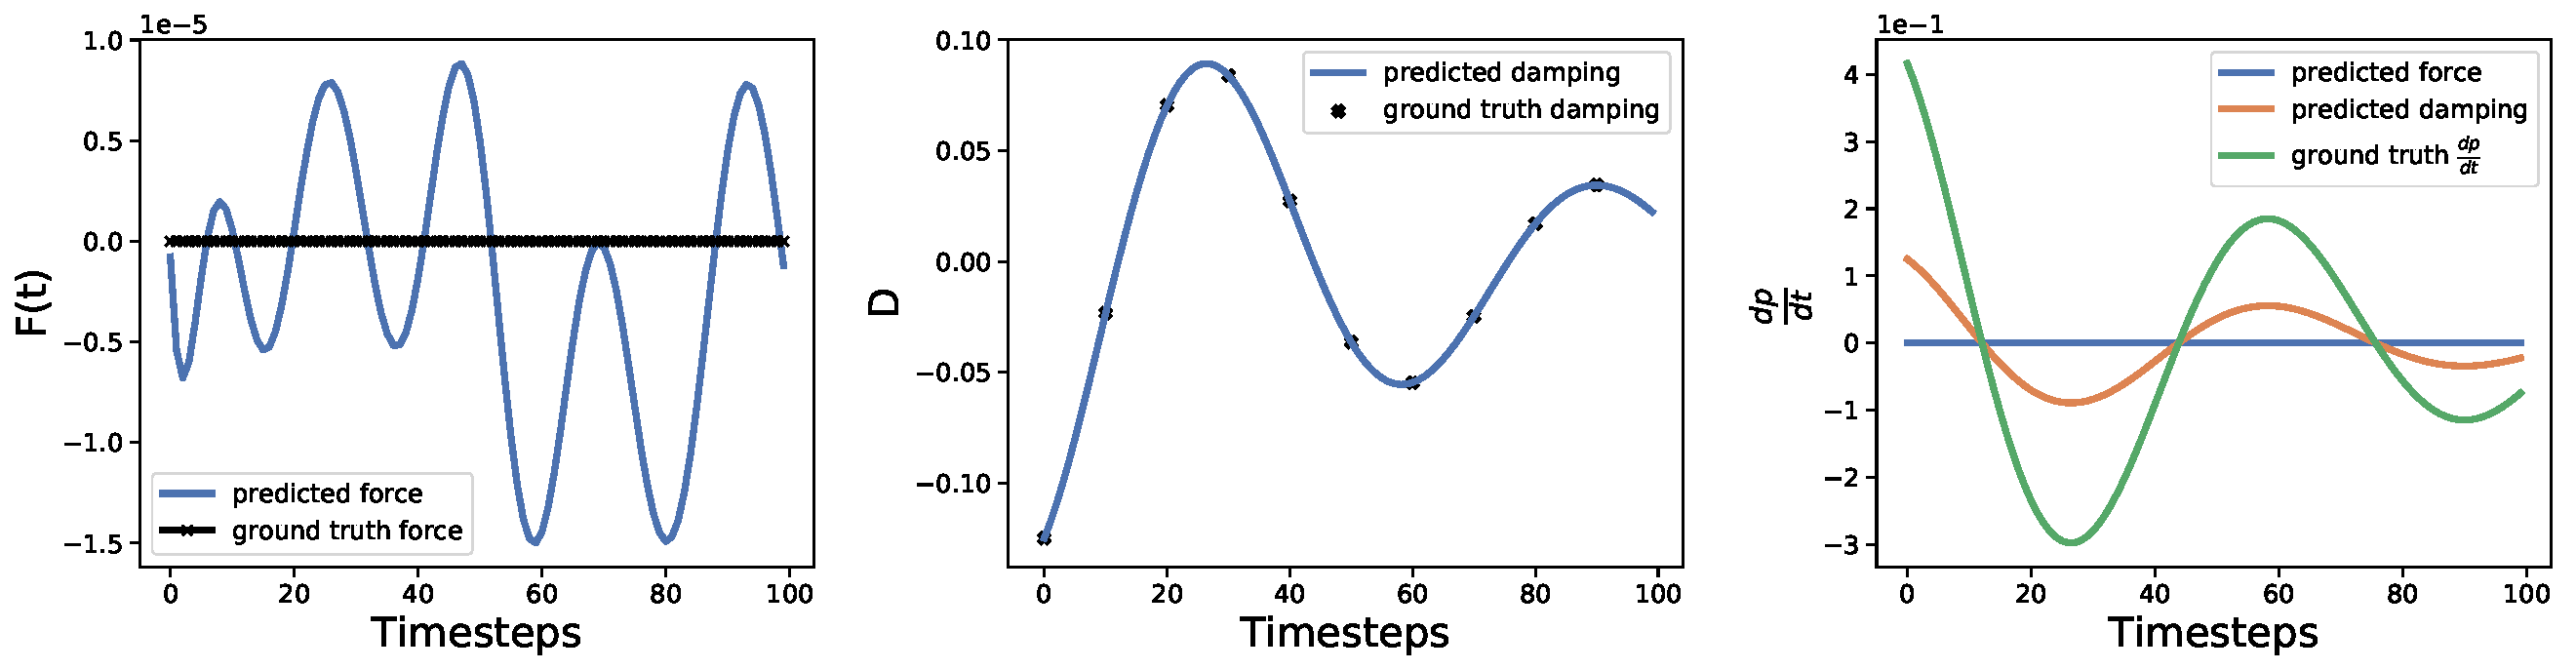
\includegraphics[width=\textwidth]{figures/figures/damped/1/damped_dpdt_0.pdf}
		\caption{Learnt Force and Damping terms and their contribution to $dp/dt$}
	\end{subfigure}
	\begin{subfigure}[b]{0.48\textwidth}
	    \centering
		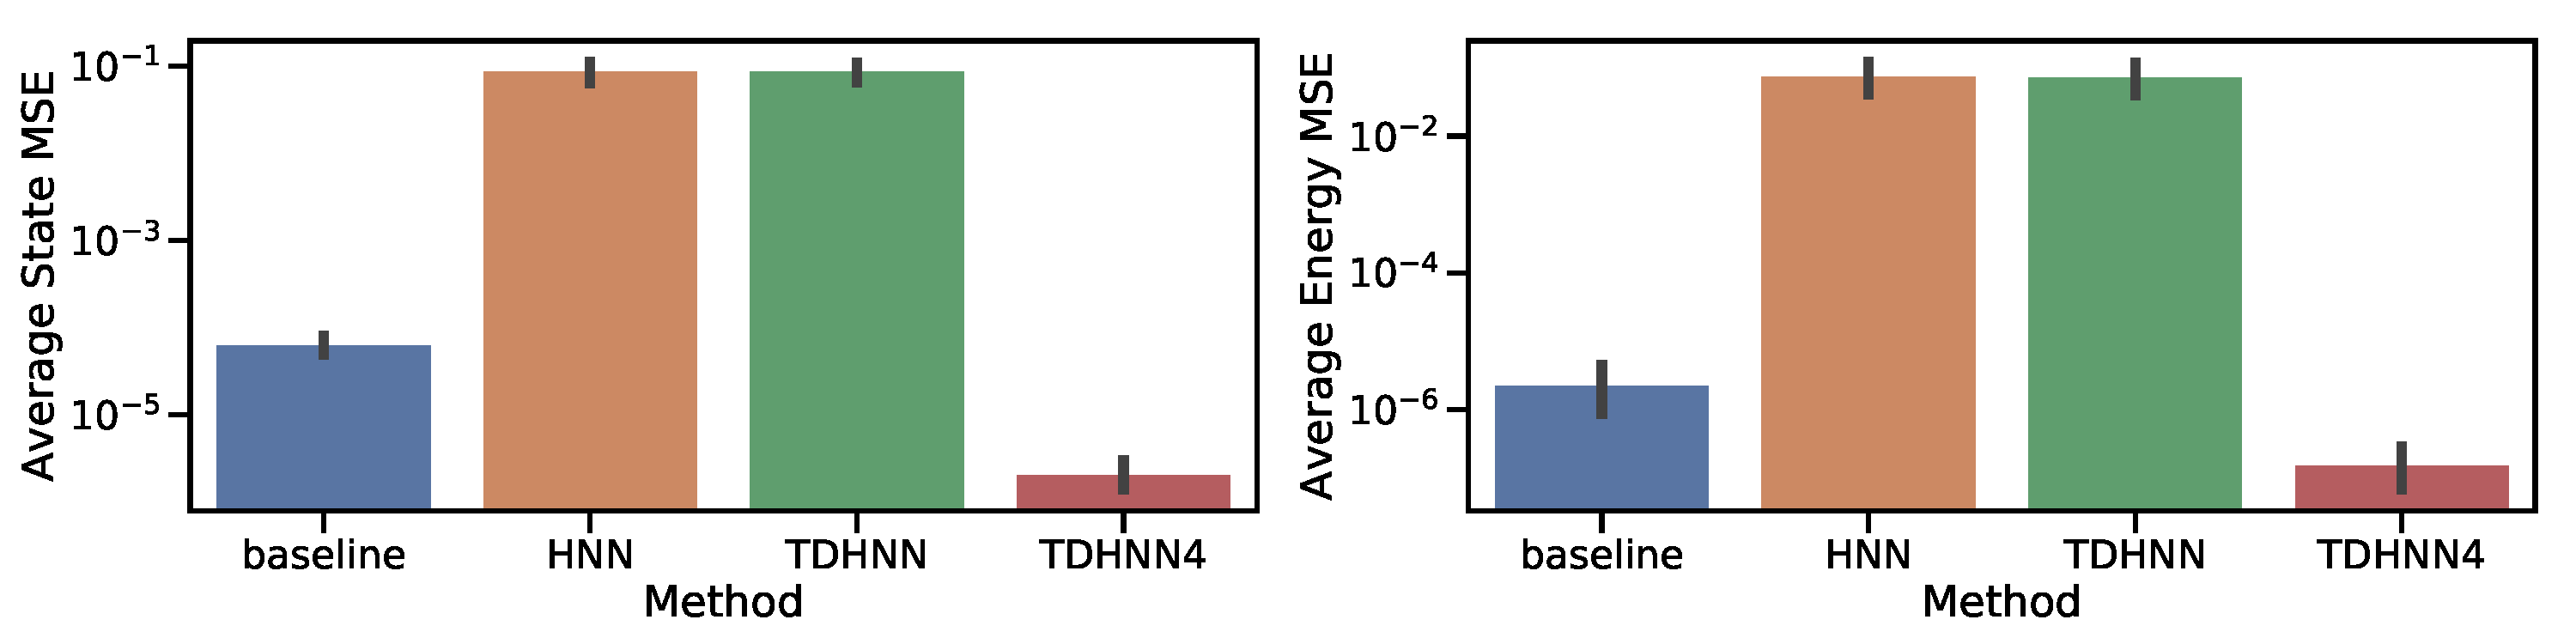
\includegraphics[width=\textwidth]{figures/figures/damped/1/damped_errors_0.pdf}
		\caption{Rollout state and energy MSE averaged across 25 initial test states}
	\end{subfigure}
\caption{Damped mass spring setting: Baseline and TDHNN4 recover the underlying dynamics. TDHNN4 is also able to accurately learn the damping coefficient since the predicted damping is indistinguishable from the ground truth.}
\label{damped}
\end{figure}

We can see that both baseline NN and TDHNN4 recover the dynamics well, whereas HNN and TDHNN struggle to learn the damping as there is no direct way of learning a Hamiltonian with damping.

\subsection{Forced Mass Spring}

Typically, while we cannot write the Hamiltonian for a damped system, we can write one for a forced system. Here, we study 2 types of forced mass-spring systems. The first has the following Hamiltonian form:
\begin{equation}
\mathcal{H} = \frac{1}{2}kq^2 + \frac{1}{2m}p^2 - qF_0\sin(\omega t) 
\end{equation}
\begin{figure}[h!]
\centering
\captionsetup{justification=centering}
%	\begin{subfigure}[b]{0.4\textwidth}
%		\centering
%		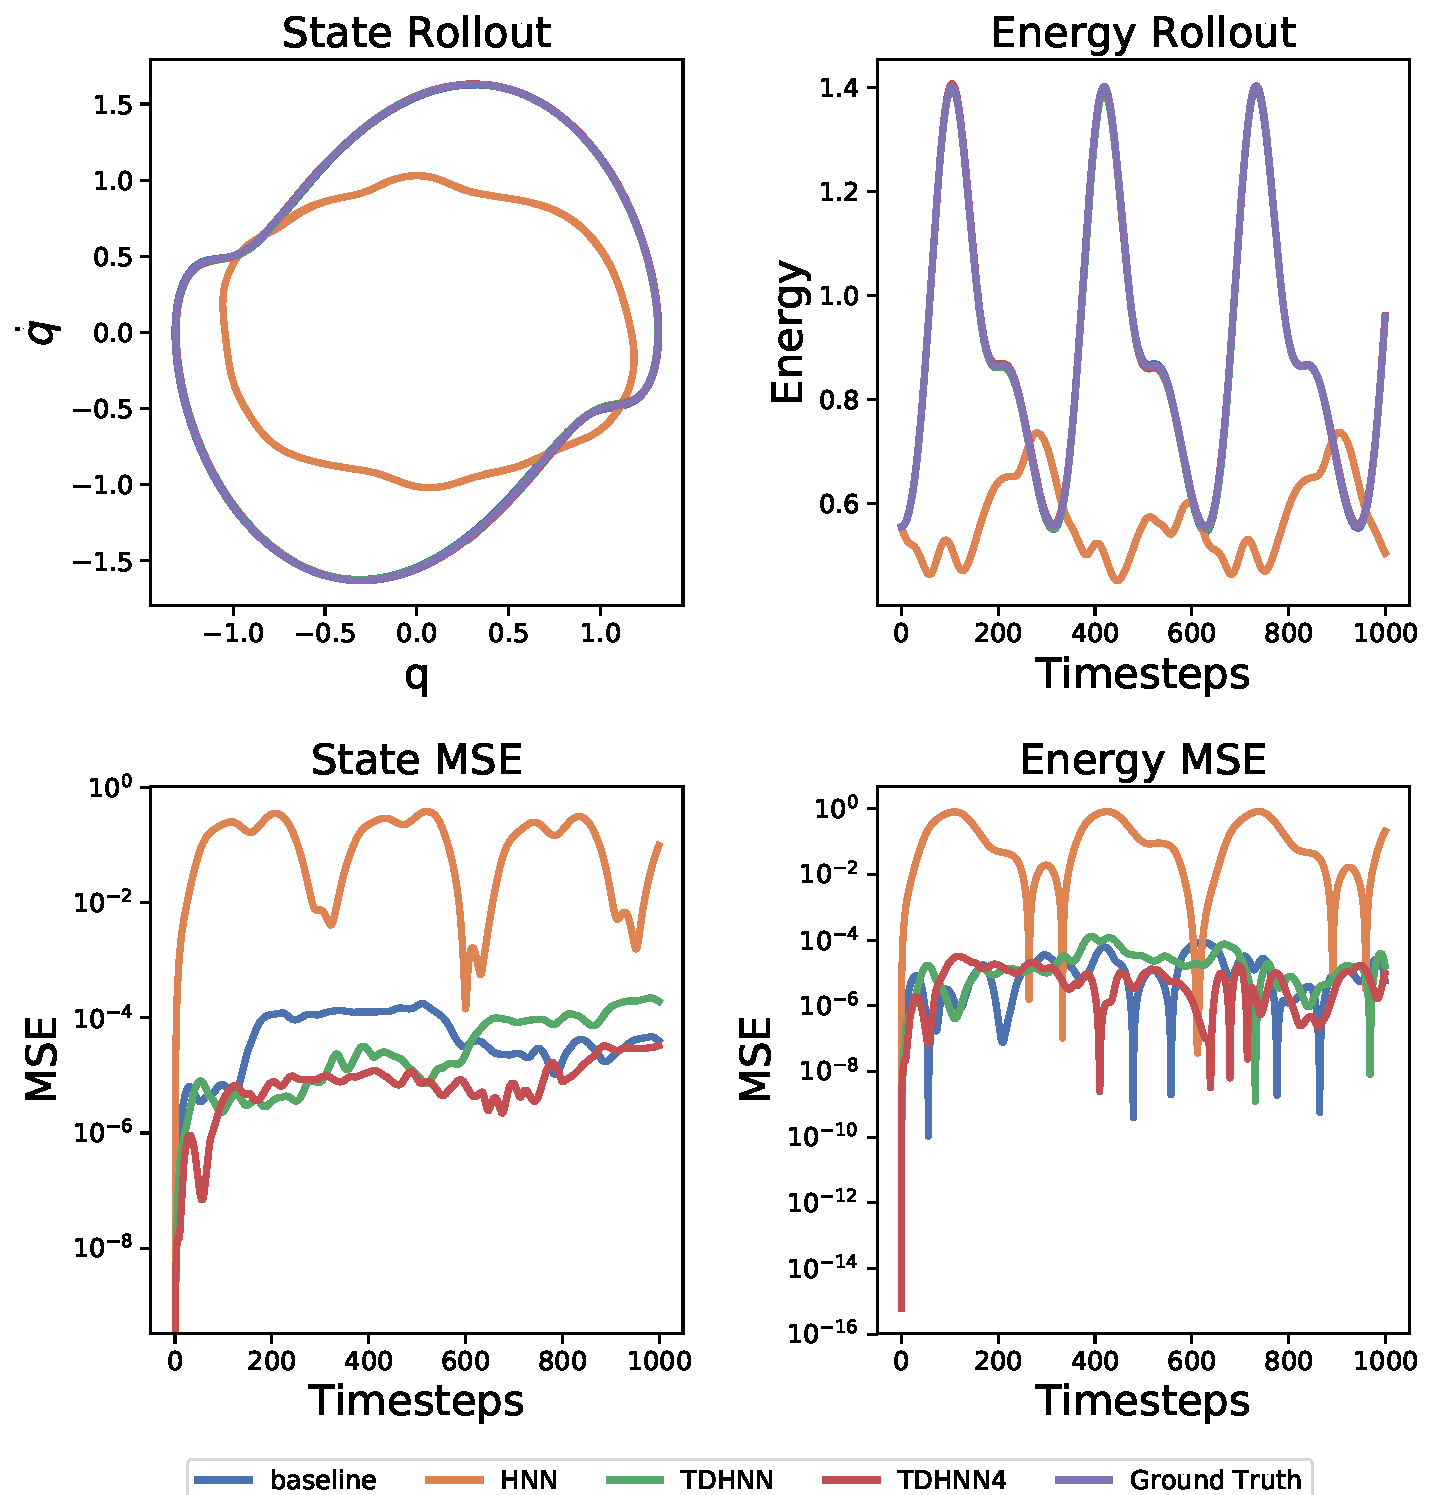
\includegraphics[width=\textwidth]{figures/forced_mass_spring_1.pdf}
%		\caption{State and energy rollout/MSE of an initial condition in the test set.}
%	\end{subfigure}
	\begin{subfigure}[b]{0.48\textwidth}
		\centering
		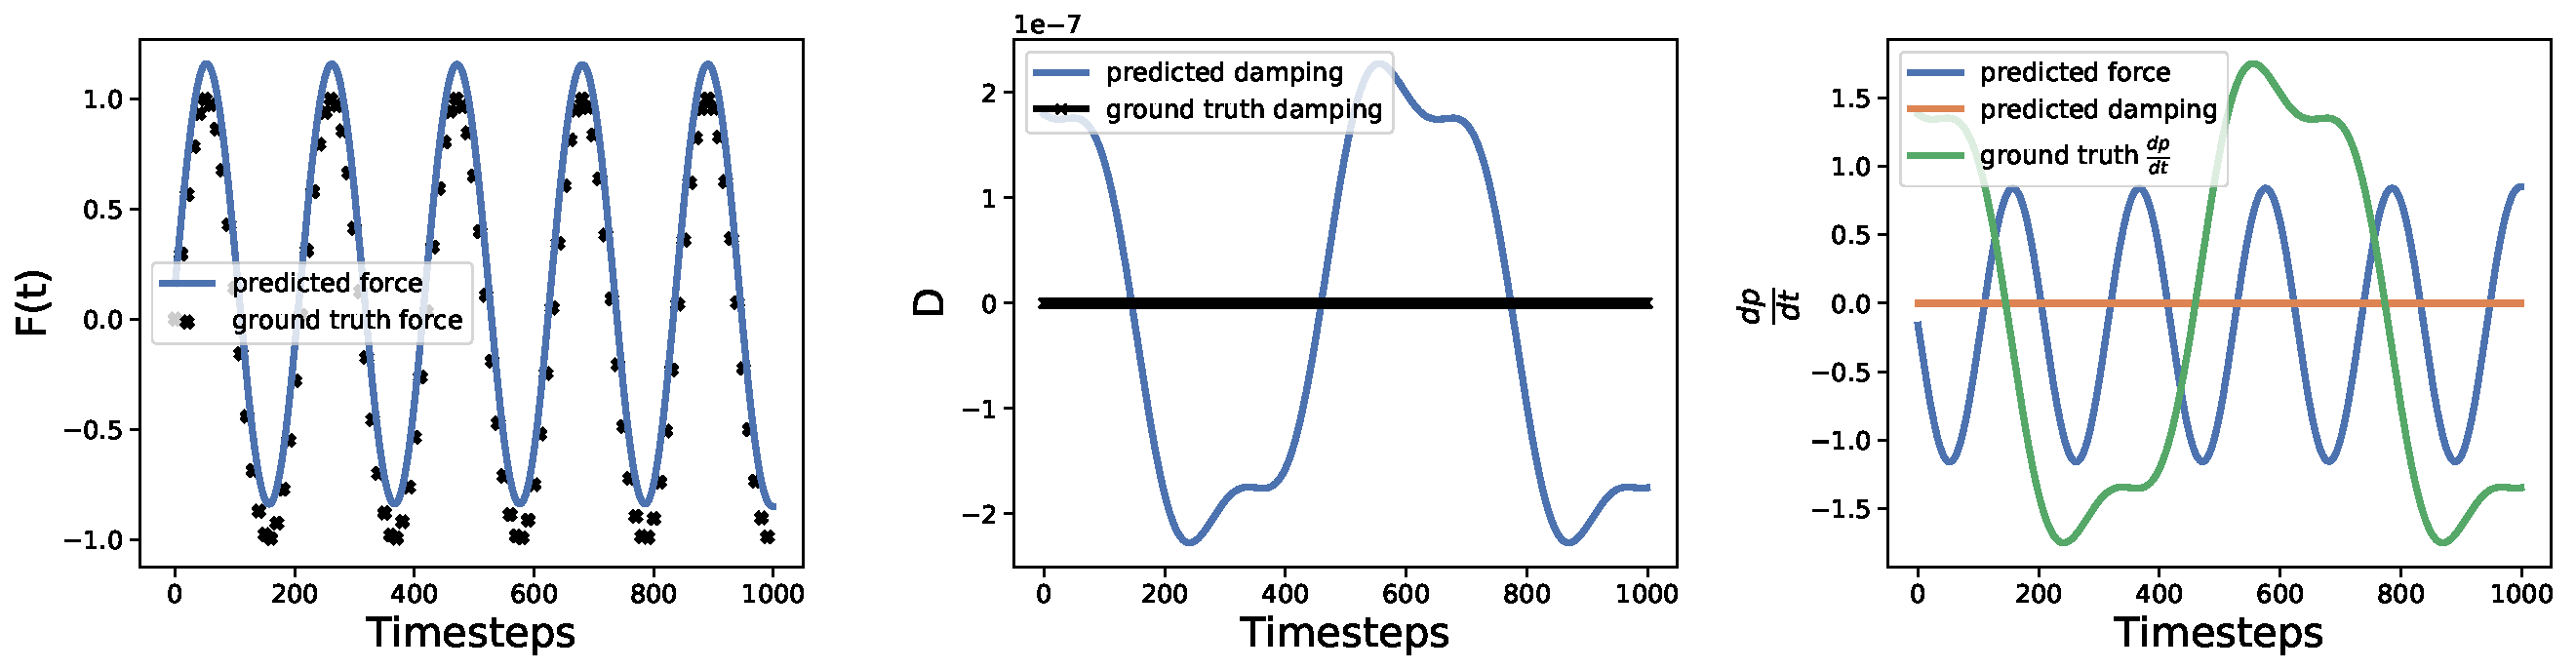
\includegraphics[width=\textwidth]{figures/figures/forced_mass_spring/1/forced_mass_spring_dpdt_0.pdf}
		\caption{Learnt Force and Damping terms and their contribution to $dp/dt$}
	\end{subfigure}
	\begin{subfigure}[b]{0.48\textwidth}
	    \centering
		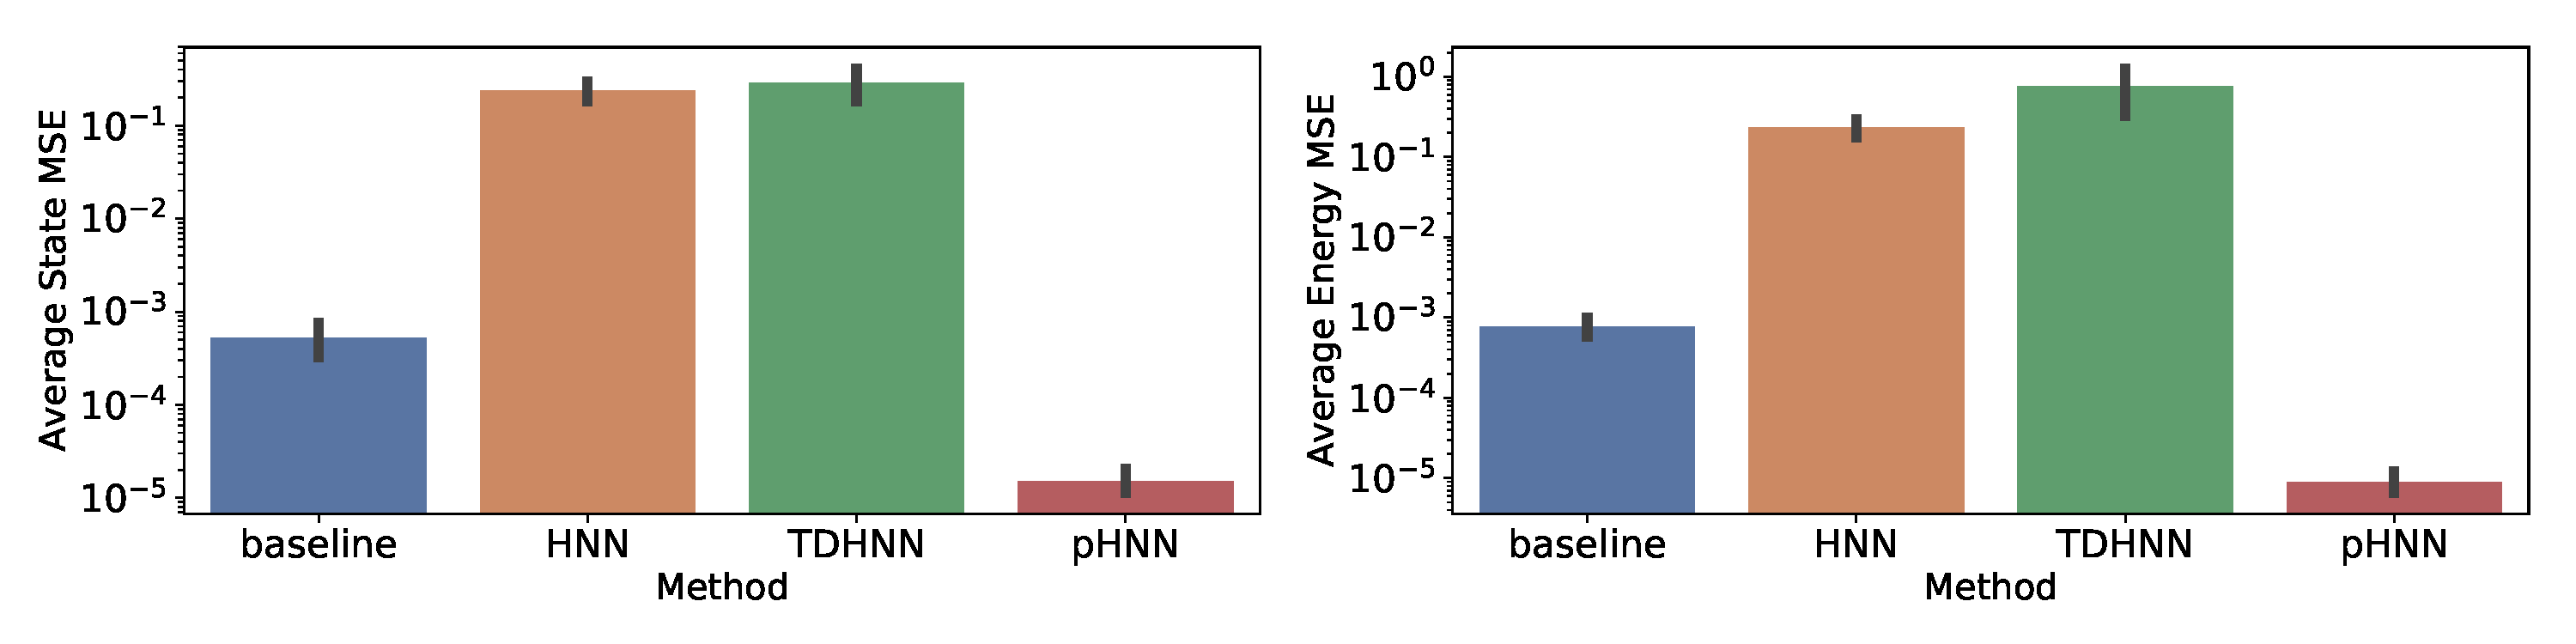
\includegraphics[width=\textwidth]{figures/figures/forced_mass_spring/1/forced_mass_spring_errors_0.pdf}
		\caption{Rollout state and energy MSE averaged across 25 initial test states}
	\end{subfigure}
\caption{Forced mass spring setting: HNN cannot learn the underlying dynamics as it has no explicit-time dependence. TDHNN4 shows the best performance as it explicitly learns a time-dependent force.}
\label{fig.fmspring1}
\end{figure}

The second has the Hamiltonian:
\begin{equation}
\mathcal{H} = \frac{1}{2}kq^2 + \frac{1}{2m}p^2 - qF_0\sin(\omega t)\sin(2\omega t)
\end{equation}
\begin{figure}[h!]
\centering
\captionsetup{justification=centering}
%	\begin{subfigure}[b]{0.4\textwidth}
%		\centering
%		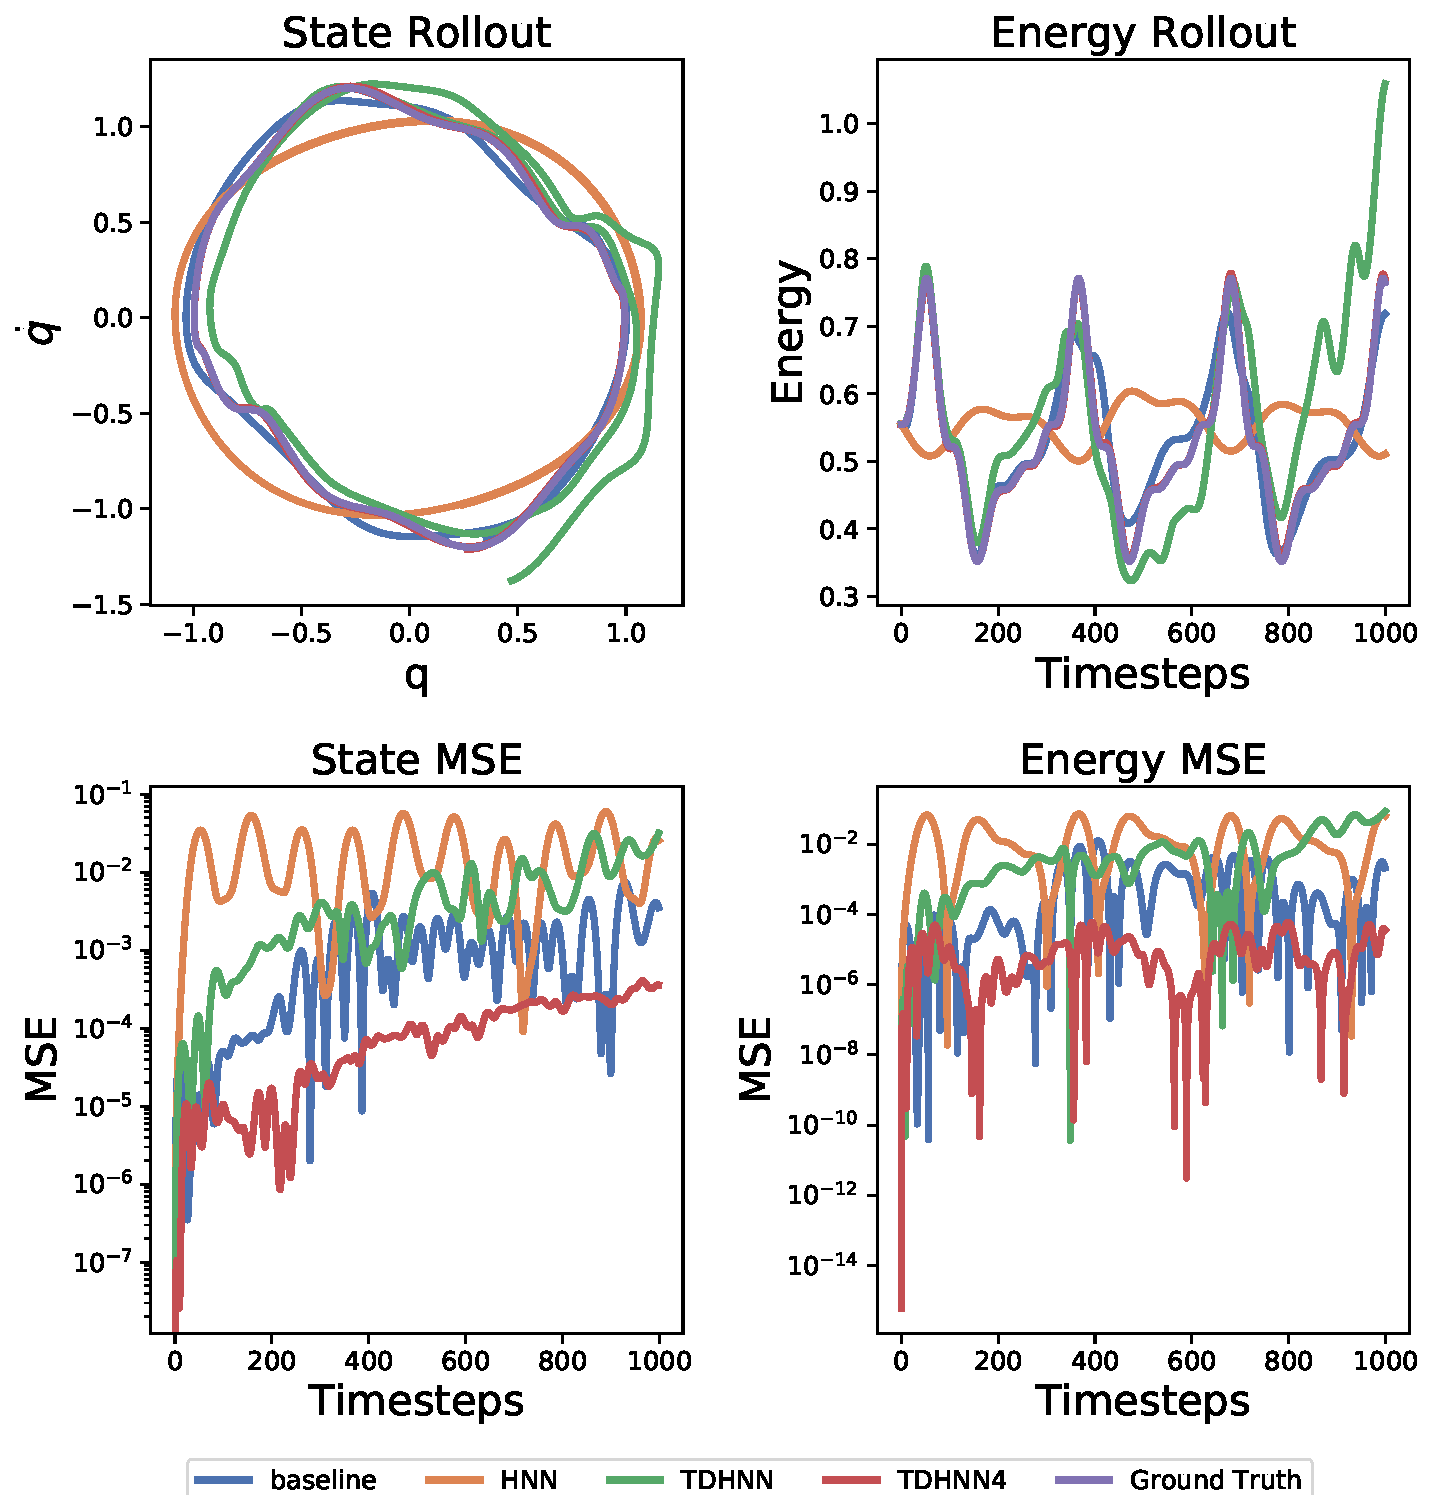
\includegraphics[width=\textwidth]{figures/forced_mass_spring_2.pdf}
%		\caption{State and energy rollout/MSE of an initial condition in the test set.}
%	\end{subfigure}
	\begin{subfigure}[b]{0.48\textwidth}
		\centering
		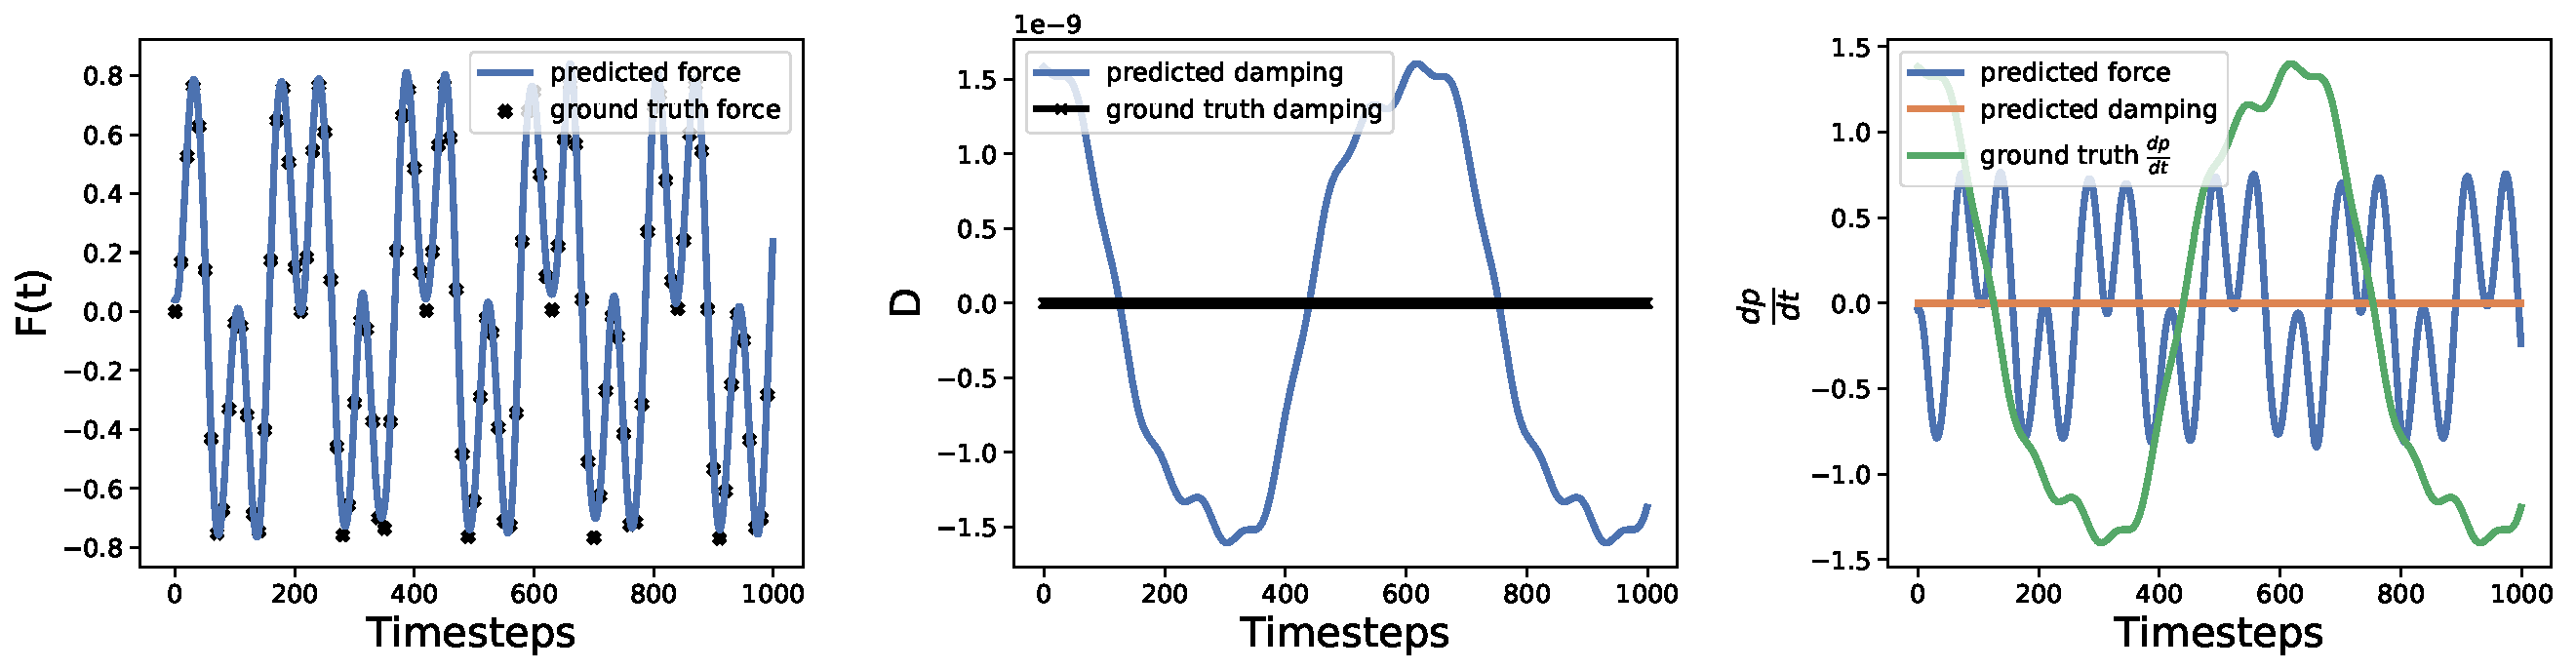
\includegraphics[width=\textwidth]{figures/figures/forced_mass_spring/2/forced_mass_spring_dpdt_0.pdf}
		\caption{Learnt Force and Damping terms and their contribution to $dp/dt$}
	\end{subfigure}
	\begin{subfigure}[b]{0.48\textwidth}
	    \centering
		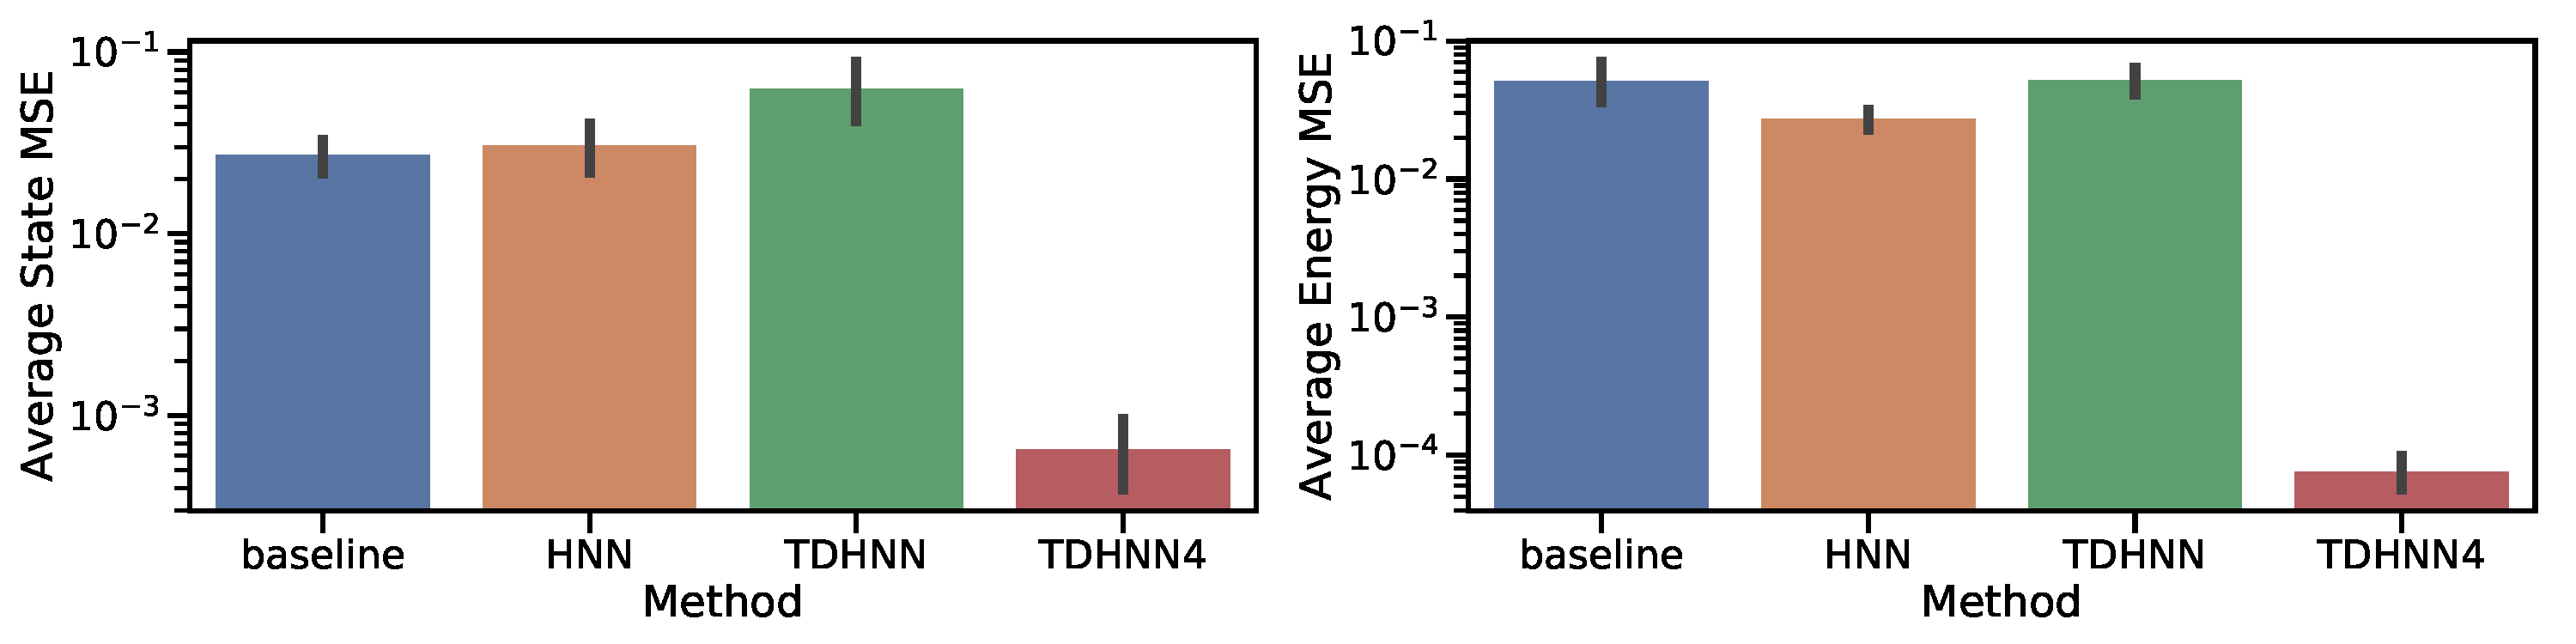
\includegraphics[width=\textwidth]{figures/figures/forced_mass_spring/2/forced_mass_spring_errors_0.pdf}
		\caption{Rollout state and energy MSE averaged across 25 initial test states}
	\end{subfigure}
\caption{The time dependent force here is non-trivial, but TDHNN4 shows it can recover it.}
\label{fig.fmspring2}
\end{figure}
\textbf{Training:} In both settings, we use 20 initial conditions, where the initial state $[q_0,p_0]$ is sampled such that $q_0^2 +p_0^2 =r_0^2$ where $1 \leq r_0 \leq 4.5$. The states are rolled out to $T_{max}=10.01$ at a $\Delta t = 0.01$. $k$, $m$ and $F_0$ are all set to 1 without loss of generality. The forcing coefficient term $\omega$ is set to 3. 

\textbf{Test:} At inference, we compute the rollout of 25 unseen initial conditions, and report the average state and energy rollout MSE in the figures \ref{fig.fmspring1} and \ref{fig.fmspring2}.

\subsection{Duffing Equation}

The general duffing equation combines both the force and damping terms discussed previously and has a non-linear potential function $V(q)$. Typically the equation is written as:

\begin{equation}
\ddot{q} = -\delta \dot{q} -\alpha q -\beta q^3 +\gamma \sin(\omega t) 
\end{equation}

One can see that the unforced and undamped regular Hamiltonian $\mathcal{H}_{reg}$ of the duffing system is:

\begin{equation}
\mathcal{H}_{reg} = \frac{p^2}{2m}+ \alpha \frac{q^2}{2} + \beta \frac{q^4}{4}
\end{equation}

This Hamiltonian therefore has a potential that can either be a single or a double well depending on the coefficients $\alpha$ and $\beta$. A combination of parameters $\alpha,\beta,\delta,\gamma,\omega$ will make the duffing system either chaotic or non-chaotic. We study both regimes.

\begin{figure}[h!]
\centering
\captionsetup{justification=centering}
%	\begin{subfigure}[b]{0.4\textwidth}
%		\centering
%		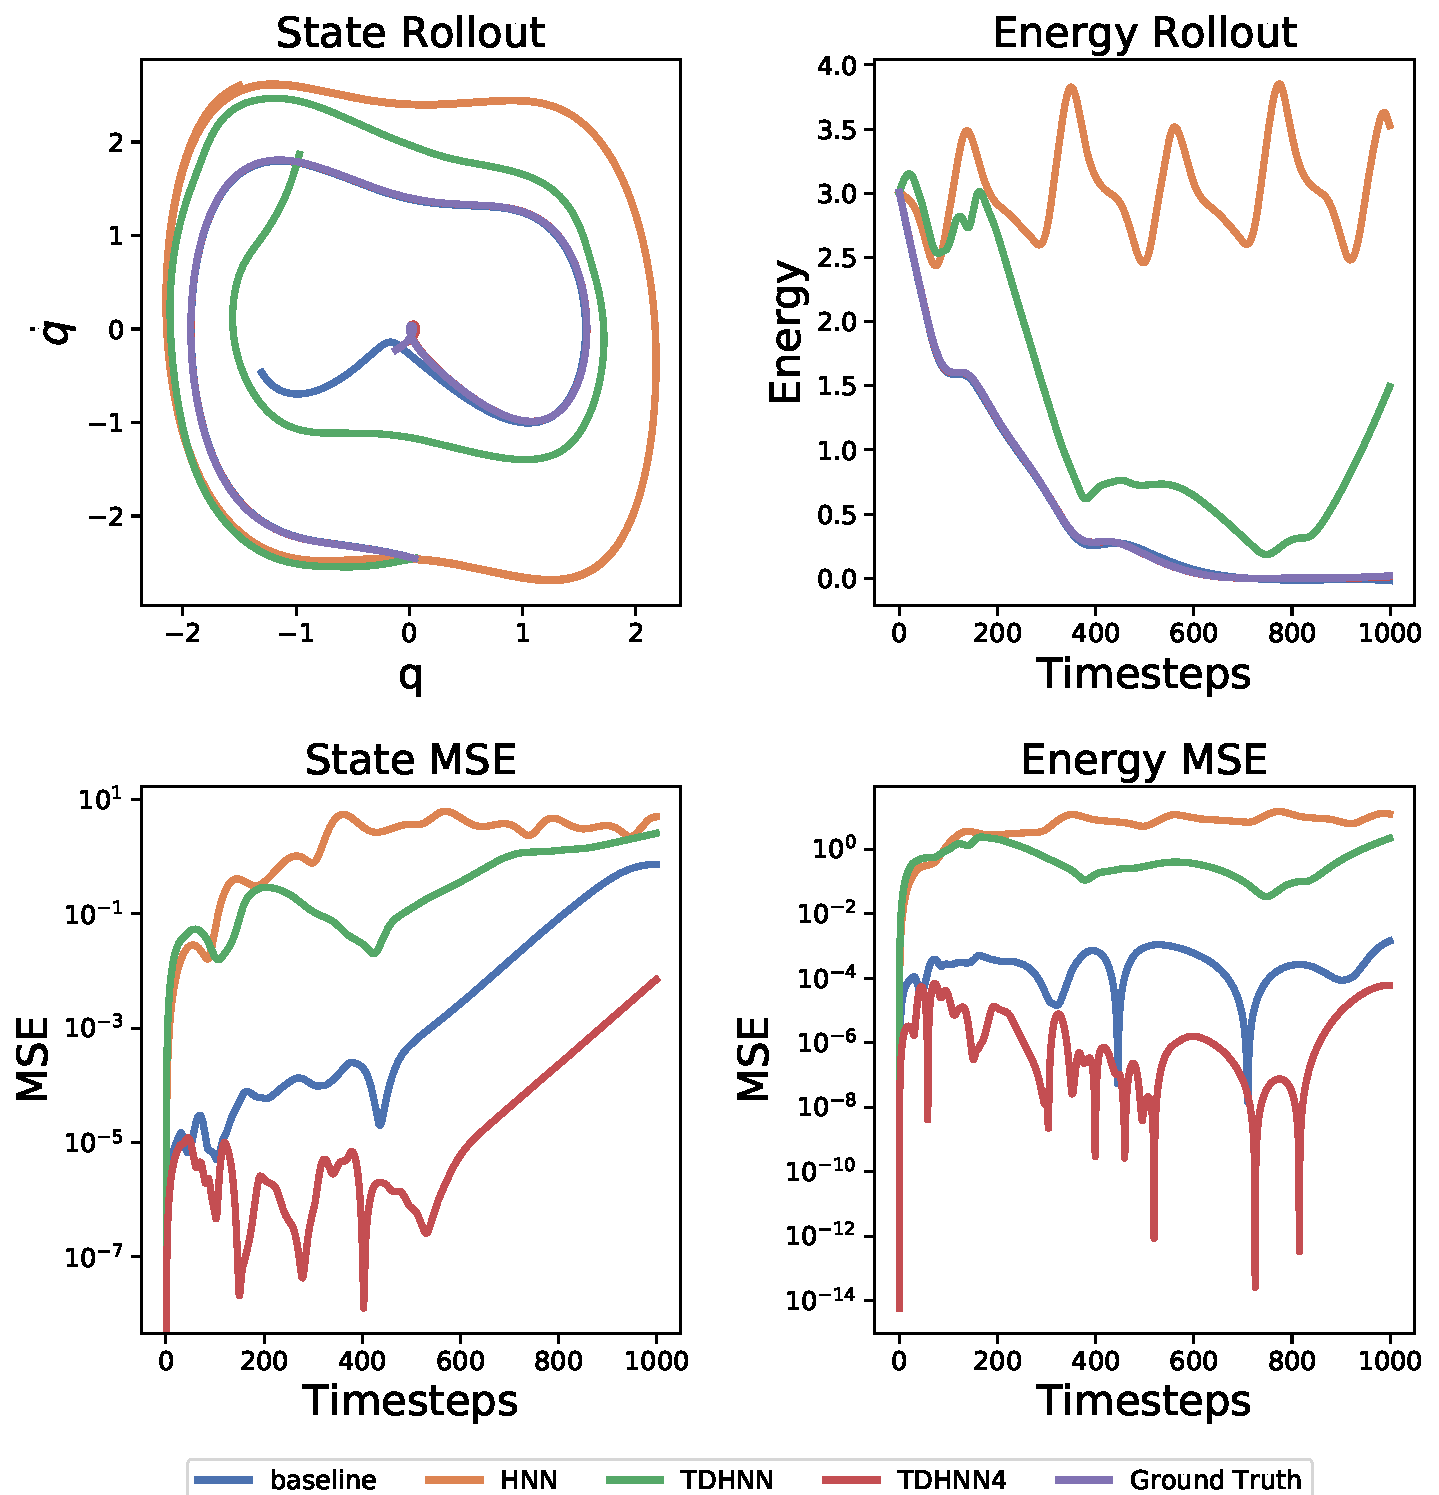
\includegraphics[width=\textwidth]{figures/duffing_state.pdf}
%		\caption{State and energy rollout/MSE of an initial condition in the test set.}
%	\end{subfigure}
	\begin{subfigure}[b]{0.48\textwidth}
		\centering
		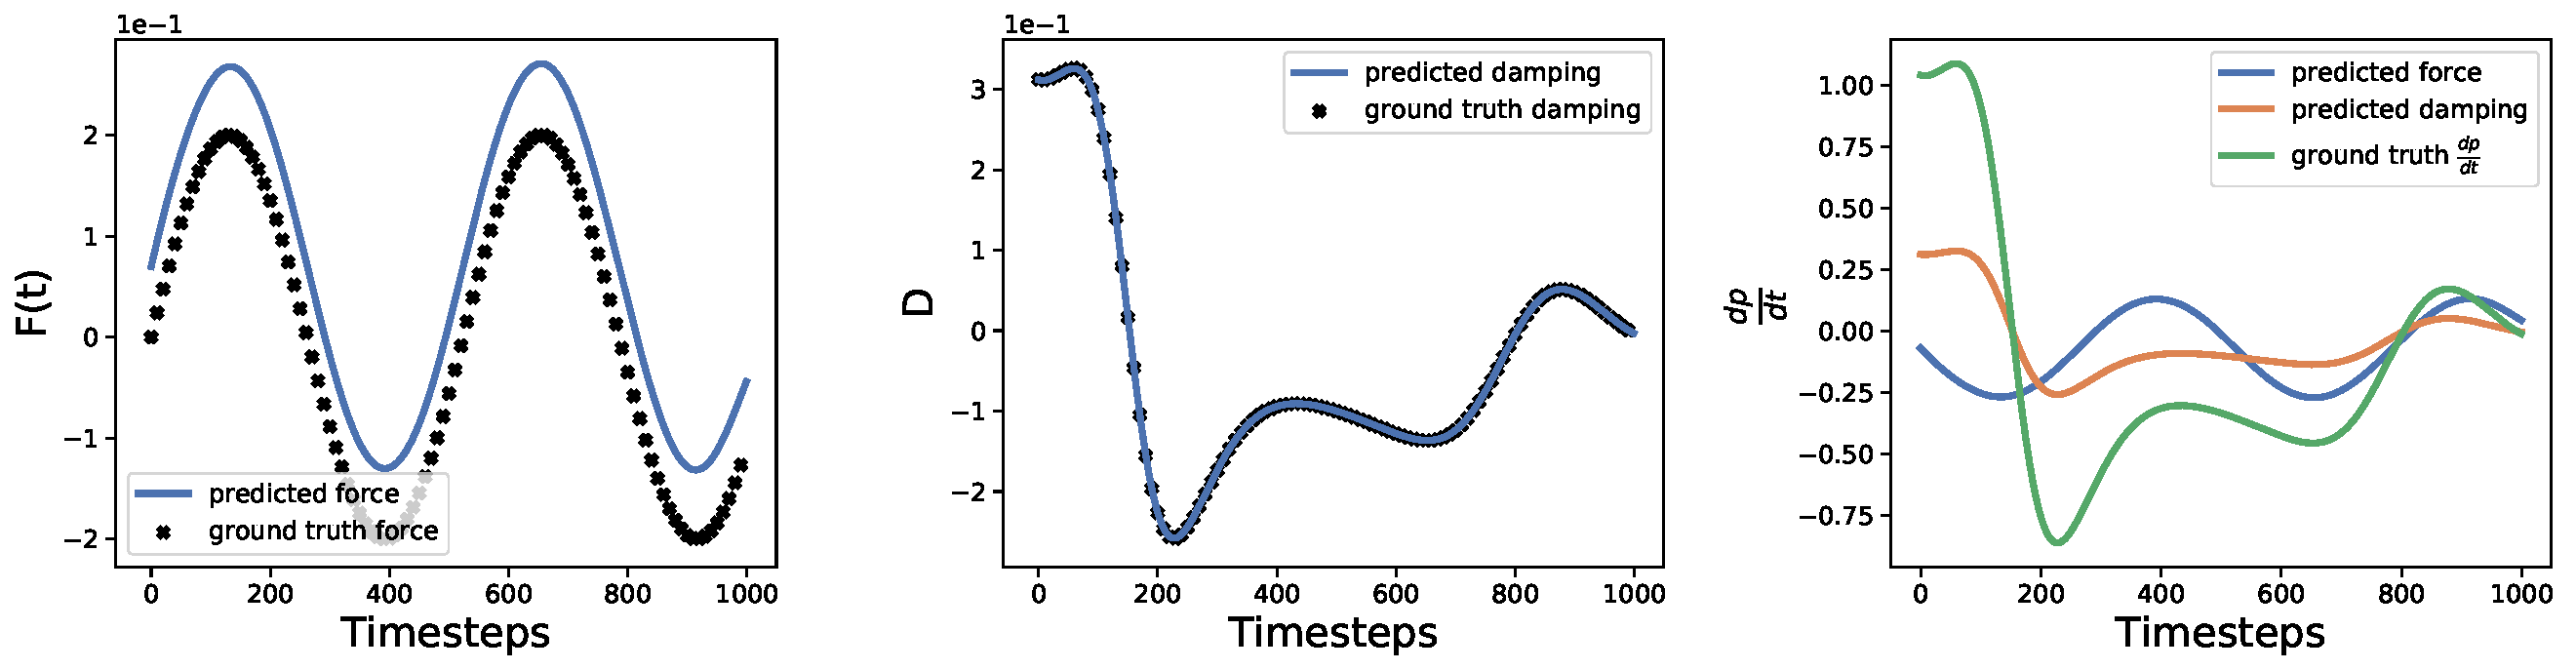
\includegraphics[width=\textwidth]{figures/figures/duffing/1/duffing_dpdt_0.pdf}
		\caption{Learnt Force and Damping terms and their contribution to $dp/dt$}
	\end{subfigure}
	\begin{subfigure}[b]{0.48\textwidth}
	    \centering
		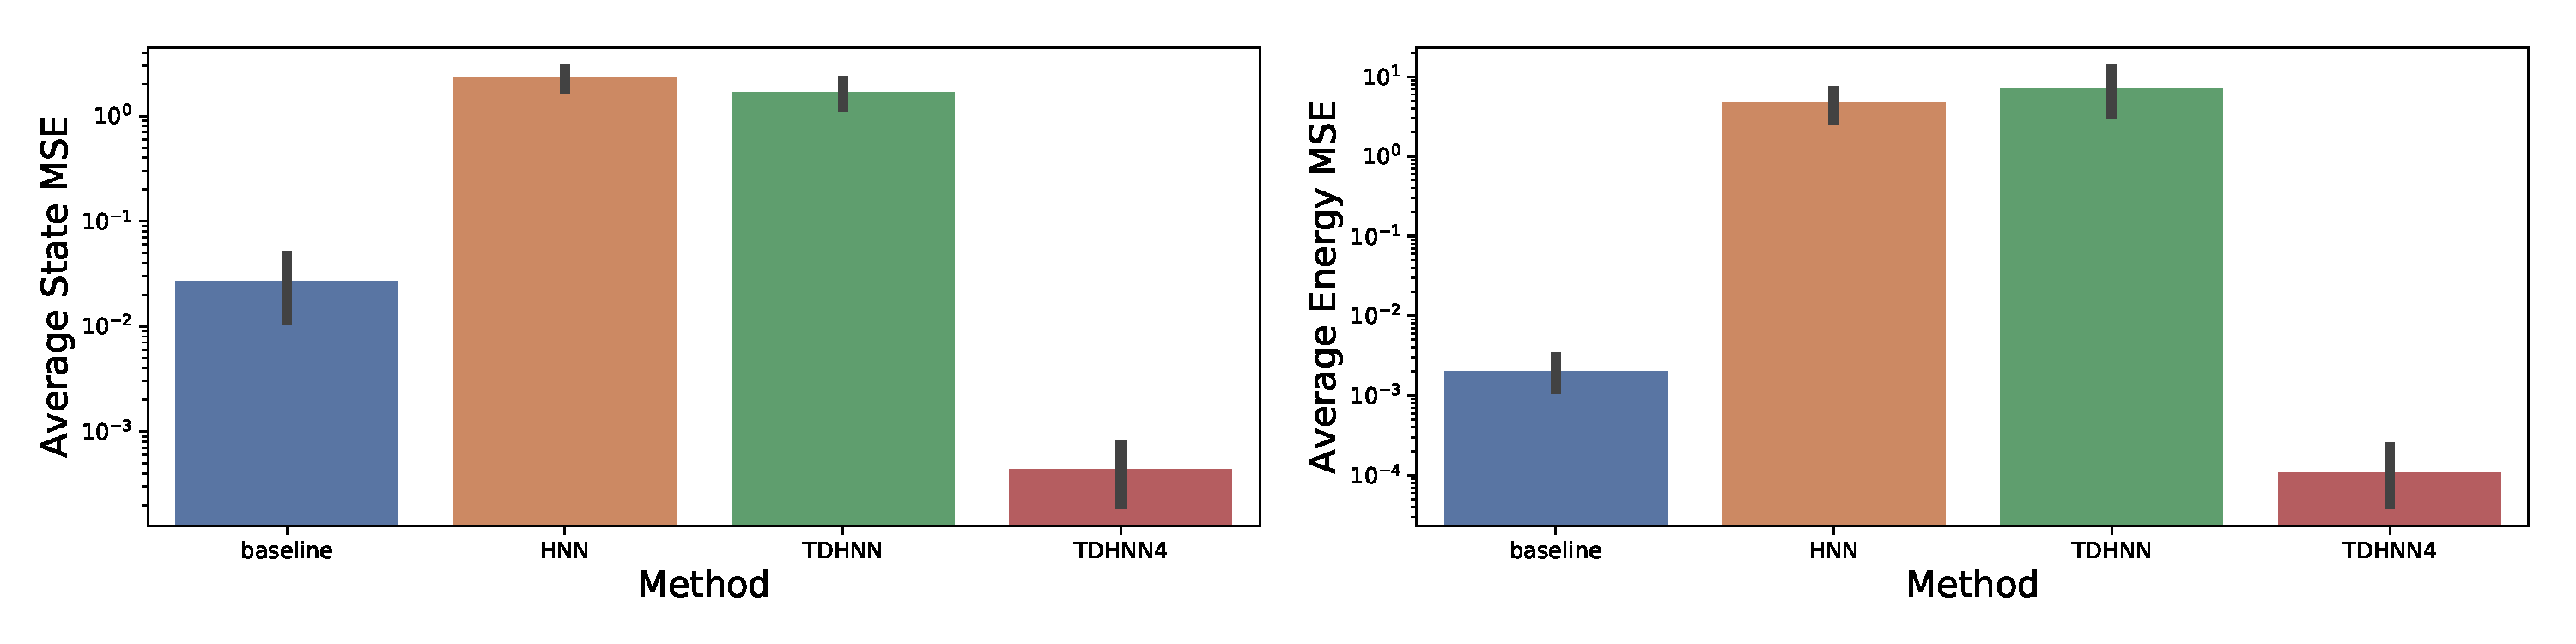
\includegraphics[width=\textwidth]{figures/figures/duffing/1/duffing_errors_0.pdf}
		\caption{Rollout state and energy MSE averaged across 25 initial test states}
	\end{subfigure}
\caption{Baseline NN and TDHNN4 both perform well in this setting. TDHNN4 is also able to extract the ground truth force and damping coefficient.}
\label{fig.duffing}
\end{figure}

\subsubsection{Non-Chaotic}

Given a set of initial parameters for the duffing equation: $\alpha =-1,\beta=1,\delta=0.3,\gamma=0.2,\omega=1.2$ we can obtain training data for the non-chaotic regime of the duffing equation. 

\textbf{Training:} We uniformly sample initial conditions in $[-1,1]^2$. We use 25 initial conditions for training, rolled out to $T_{max}=10.01$ and $\Delta t =0.01$ for the non-chaotic regime. 

\textbf{Test:} We integrate 25 unseen initial conditions at inference using the same conditions as above and evaluate both energy and state MSE (see Fig.\ref{fig.duffing}).

In addition to learning the force and damping terms accurately, inspecting the predicted Hamiltonian over a 2-D grid of position and momentum values shows that TDHNN4 can also accurately learn the $\mathcal{H}_{reg}$ term (see Fig.\ref{duffing_ham}).

\subsubsection{Chaotic}

In the chaotic regime we use the following parameters:
$\alpha =1,\beta=1,\delta=0.1,\gamma=0.39,\omega=1.4$. 

\textbf{Training:} 20 initial conditions, sampled uniformly in $[-1,1]^2$ each rolled out for one period $T=2\pi/\omega$ where $\Delta t = T/100$. This results in 2000 training points.

\textbf{Test:} We test our system by assessing whether it is visually able to recover the ground truth Poincar\'e section of an initial condition. The Poincar\'e map of a trajectory is measured by plotting the position and momentum values at regular intervals governed by the period of the forcing term. For example, a simple mass spring will generate a single dot in phase space when measured at regular intervals. To visually asses the performance of our network through a Poincare map, we test the system on a single initial condition not in the training set rolled out to $T_{max} = 18,000$ with the same $\Delta t$ as training. In order to integrate our system to such a large $T_{max}$ we work under the assumption that we have explicit knowledge of the period, and as such, we modulo the time variable with the period. This is necessary as the models are not explicitly trained on time steps beyond $2\pi/\omega$. Our results are visually presented in Fig.\ref{fig.chaos1}. The outcome suggests that TDHNN4 can indeed be used to identify chaos even after being trained with only a few data points from a chaotic trajectory. We believe this is a deeply powerful result in helping us identify chaotic trajectories.

\begin{figure}[h!]
\centering
\captionsetup{justification=centering}
%	\begin{subfigure}[b]{0.4\textwidth}
%		\centering
%		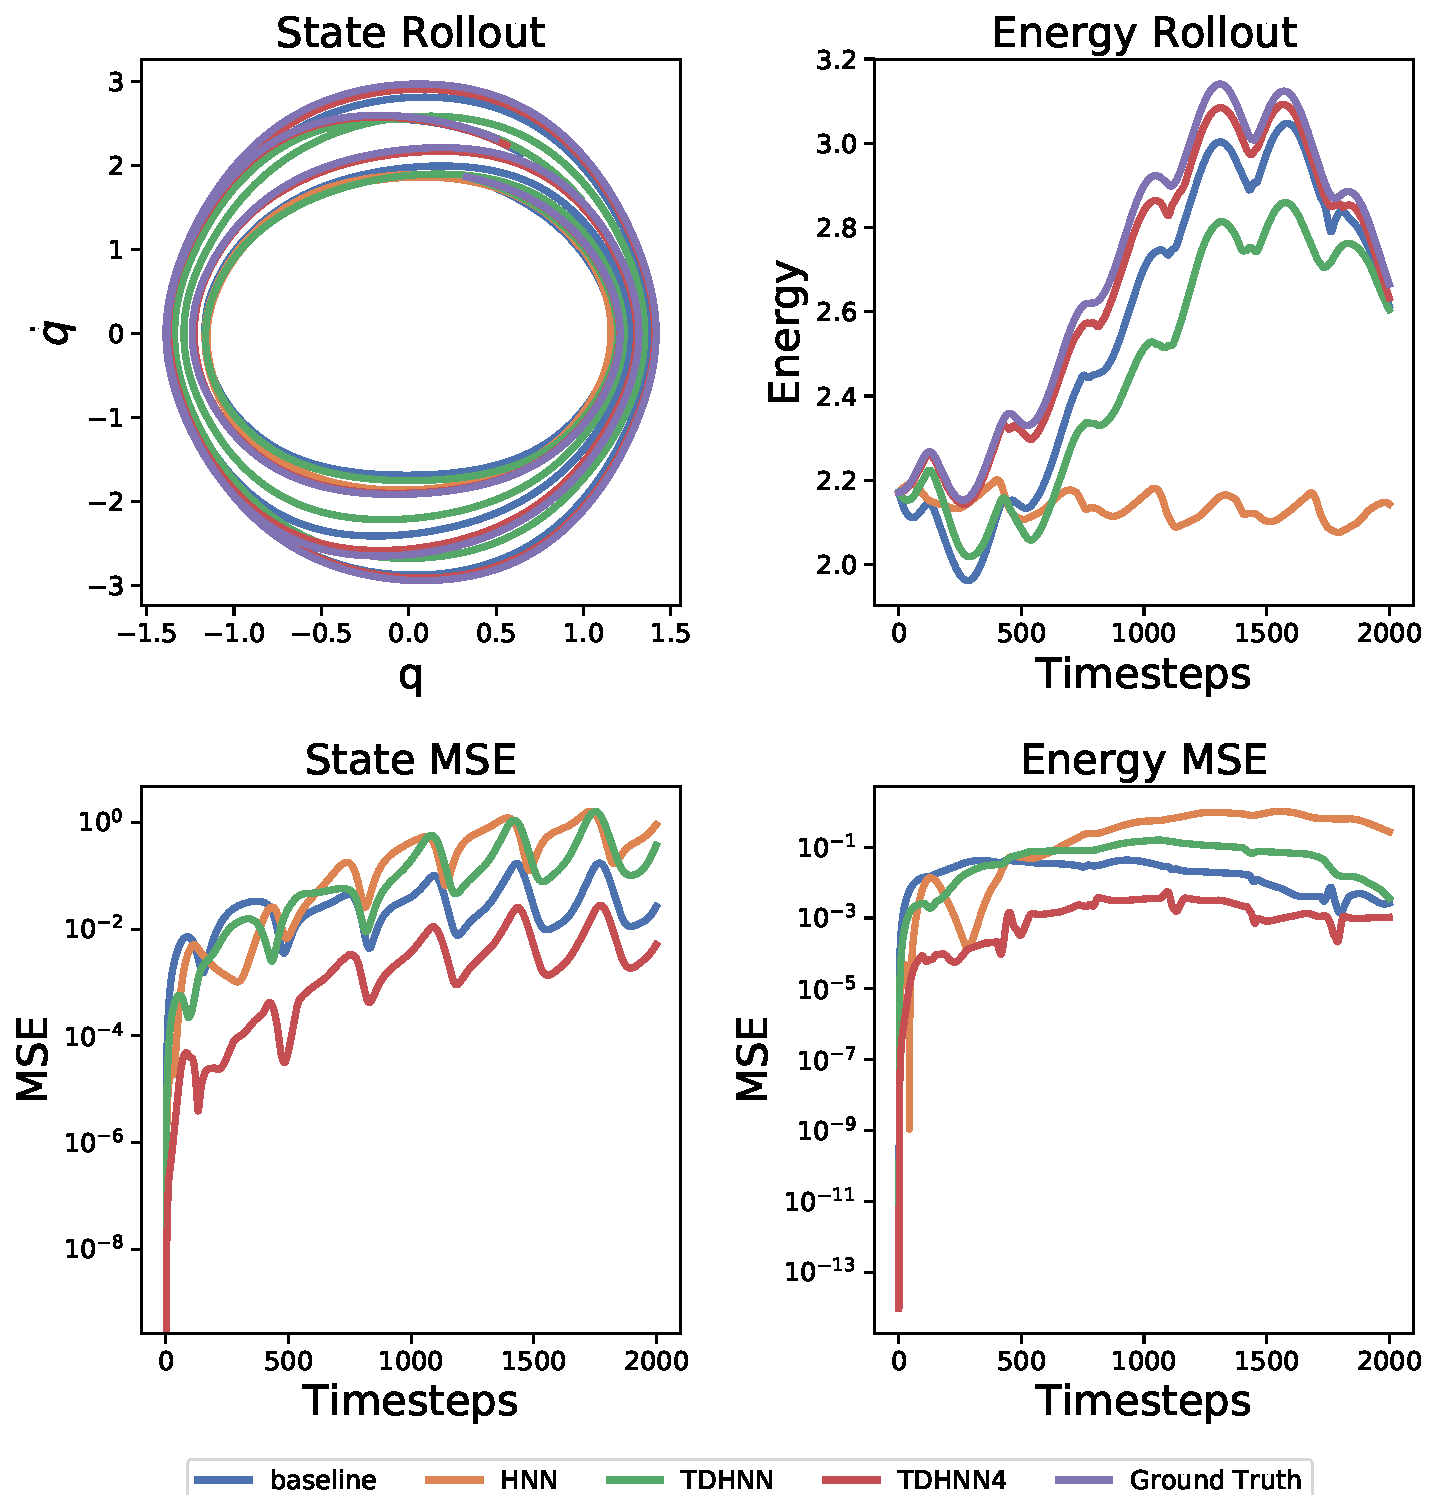
\includegraphics[width=\textwidth]{figures/relativity_pred.pdf}
%		\caption{State and energy rollout/MSE of an initial condition in the test set.}
%	\end{subfigure}
	\begin{subfigure}[b]{0.48\textwidth}
		\centering
		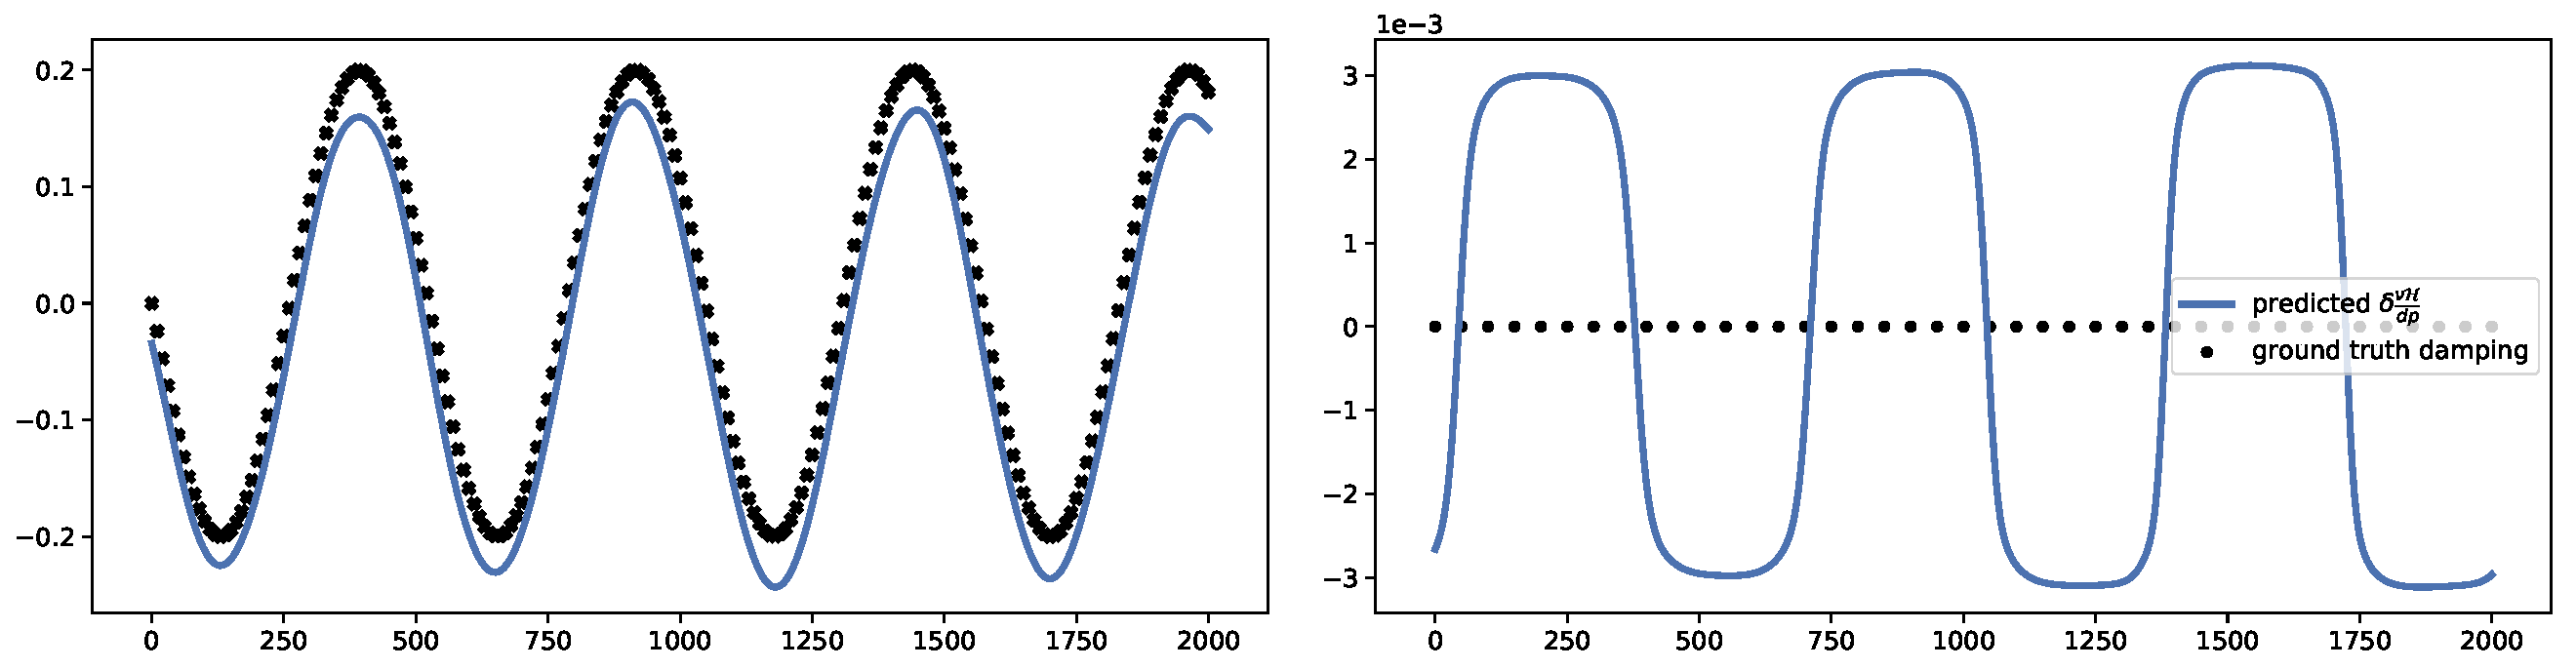
\includegraphics[width=\textwidth]{figures/figures/relativity/1/relativity_dpdt_0.pdf}
		\caption{Learnt Force and Damping terms and their contribution to $dp/dt$}
	\end{subfigure}
	\begin{subfigure}[b]{0.48\textwidth}
	    \centering
		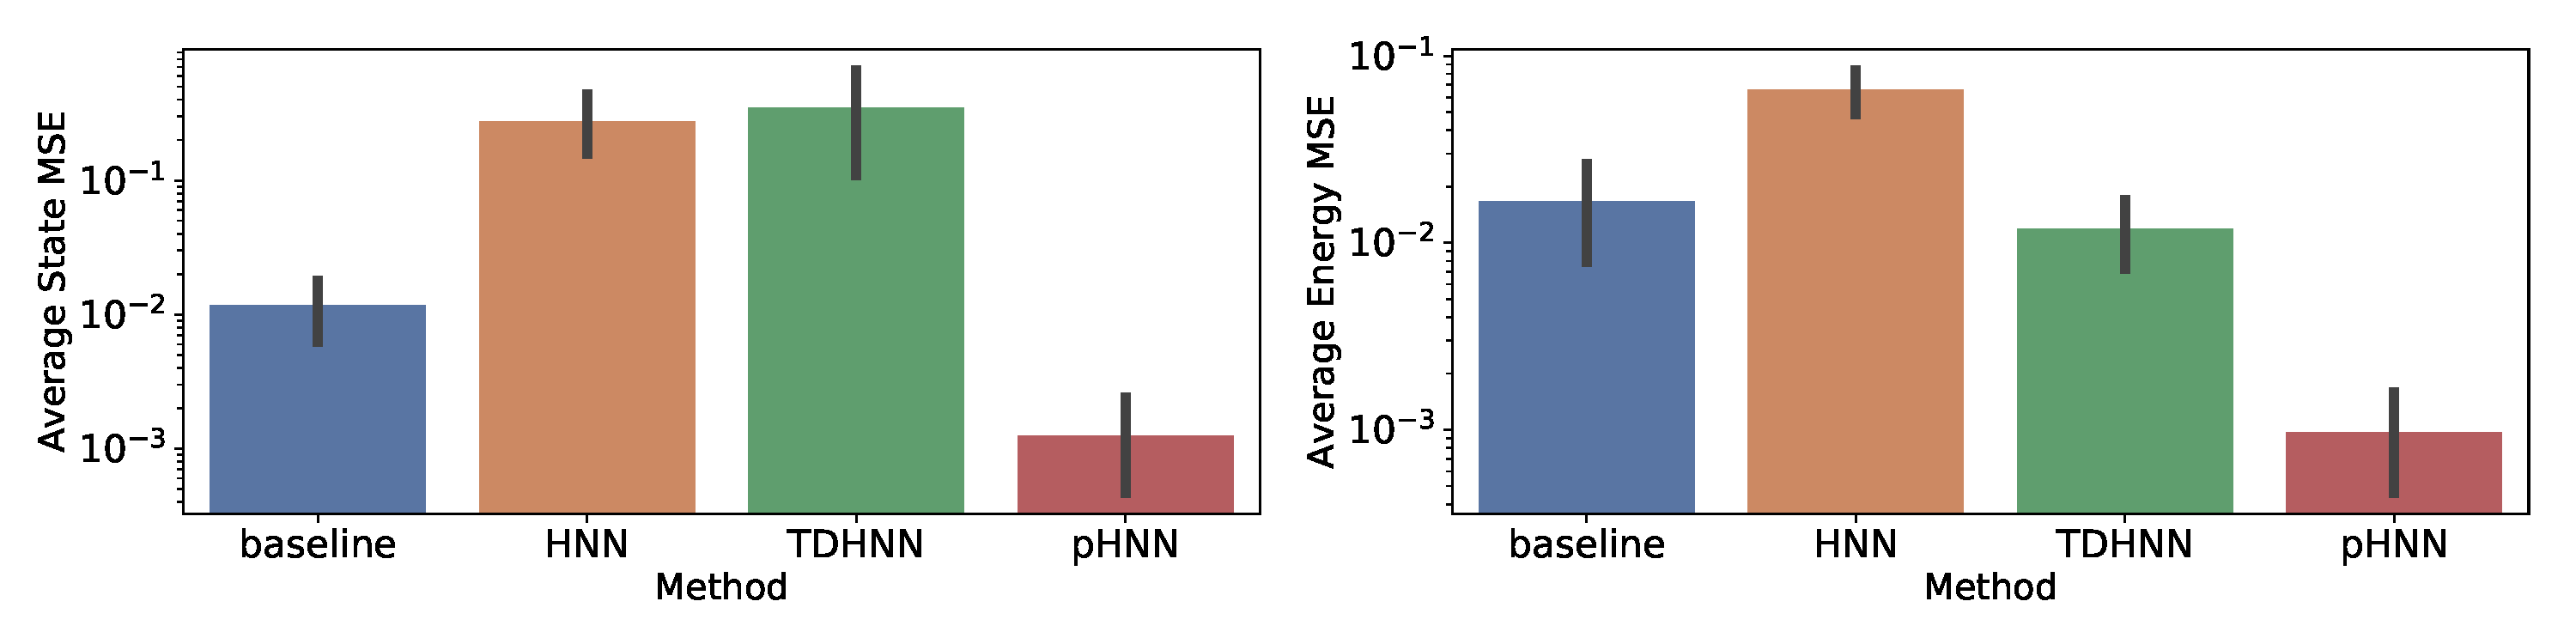
\includegraphics[width=\textwidth]{figures/figures/relativity/1/relativity_errors_0.pdf}
		\caption{Rollout state and energy MSE averaged across 25 initial test states}
	\end{subfigure}
\caption{Learned dynamics of a relativistic duffing system.}
\end{figure}
\subsection{Relativity}
We investigate the duffing equation in a special relativistic framework. The Hamiltonian under consideration is:
\begin{equation}
\mathcal{H} =  c\sqrt{p^2 +m_0^2c^2} + \frac{\alpha}{2}q^2 +\frac{\beta}{4}q^4 - q\gamma\sin(\omega t)
\end{equation}
where c, the speed of light is typically set to 1. For simplicity, we also set $m=1$ though our framework naturally accounts for other values.

\textbf{Training:} We train on 25 initial conditions, sampled in $[0,2]^2$ uniformly. $T_{max} = 20.01$ and $\Delta t = 0.01$. We set parameters such that $\alpha =1, \beta =1,\delta =0,\gamma = 0.2,\omega = 1.2$.

\textbf{Test:} Using the same parameters as training, we rollout 25 unseen initial conditions and compute their state/energy MSE.

\section{Discussion}

We have shown that TDHNN4 can not only outperform other approaches in learning complex physical systems but can also help us recover the underlying force and damping terms of non-autonomous systems. One challenge in achieving this result is fine-tuning the $\alpha$ and $\beta$ regularisation coefficients for the force and damping. In the duffing setting where we have both terms, it is possible to learn a shifted force i.e. $F = F_0 + \epsilon$. Upon inspection we find that such a shift is induced by heavy regularisation of the forcing term. In other words, the Hamiltonian absorbs some of the information of the forcing term. We mitigate this problem by setting small $< 10^{-8}$ regularisation coefficients in settings where we do identify a significant non-zero forcing and damping term.

In many settings we find that the classic Hamiltonian Neural Network approach or its time-dependent variant simply do not perform as well as TDHNN4 or baseline. We believe this is predominantly due to the fact that HNN and TDHNN attempt to enforce Hamilton's equations in settings where they cannot be satisfied.

While it may be argued that the method is constrained to learning and prediction within the training time horizon, we believe our method is still versatile at informing us of a periodic forcing (since we can inspect the force over time). This in turn can readily be used to renormalize the time variable at periodic intervals to integrate the system beyond the training time.
\begin{figure*}[h]
\centering
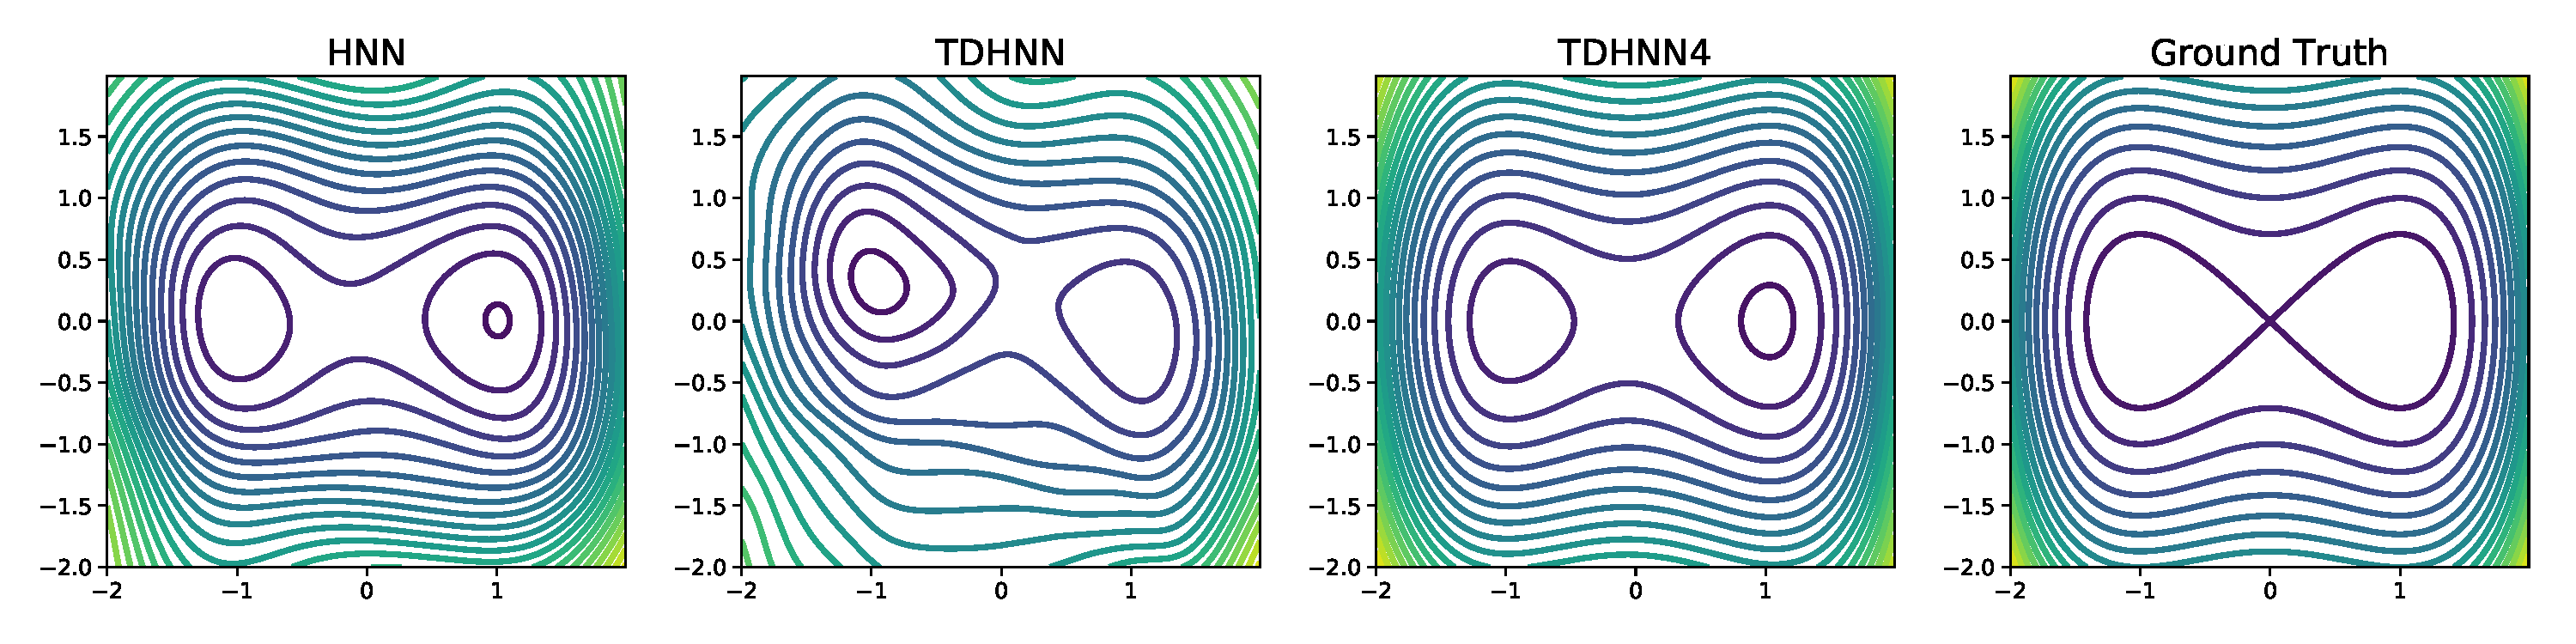
\includegraphics[width=0.9\textwidth]{figures/duffing_ham_1.pdf}
\caption{Learnt $\mathcal{H}_{reg}$ components across methods in the non-chaotic duffing setting. HNN and TDHNN learn distorted Hamiltonians that strongly depend on the input time-variable.}
\label{duffing_ham}
\end{figure*}

\section{Conclusion}

We have shown that learning the dynamics of time-dependent non-autonomous systems can be achieved with TDHNN4, a versatile neural network embedded with a port-hamiltonian designed to recover the underlying Hamiltonian, Damping and Forcing terms. We show that such an approach, unique in its own right, outperforms naive extensions of existing methods. We believe this work forms a strong basis for further advances in learning complex systems including, but not limited to, chemical bond forces and controlled dynamics. 
%\section{Questions/Thoughts}

%\begin{enumerate}
%\item At present, baseline,HNN and TDHNN all use 3 layers with 200 weights per layer. TDHNN does the same to compute H, but it also has a separate network that learns F. Some could argue this is not fair - so how can we be 'fair' in our comparison?
%\item The math does not checkout for the shifted force - should we keep trying to tune parameters so that force isn't offset? Note: even dissipative SympODEN learn a shifted force
%\item we need to finalize the name for TDHNN4 as well as the title?
%\item do we plan to arxiv this soon - to avoid the scoop?
%\item does it suffice to investigate the mass spring system almost exclusively?
%\item can we explain why baseline does surprisingly well with damping and duffing? Somehow dissipation seems to help the baseline. 
%\end{enumerate}

\pagebreak

\bibliography{references.bib}

\onecolumn
\section*{Appendix}

\subsection*{A.1}

Why can we not including damping into the Hamiltonian? Let us take the following damped system:
\begin{equation}
\ddot{\mathbf{q}} = -\mathbf{q} - \delta\dot{\mathbf{q}}
\end{equation}
where we know $\mathbf{p}=m\dot{\mathbf{q}}$ which implies $\dot{\mathbf{q}} = m^{-1}\mathbf{p}$.

Then, the integral of the right hand side with respect to q will give us:

\begin{equation}
\frac{\mathbf{q}^2}{2} + \delta \mathbf{q} \dot{\mathbf{q}}
\end{equation}

The equation above looks like a modified potential function which can be combined with a kinetic energy term to give a Hamiltonian s.t.:

\begin{equation}
\mathcal{H} =\frac{ \mathbf{p}^2}{2m} + \frac{\mathbf{q}^2}{2} + \delta \mathbf{q} \dot{\mathbf{q}}
\end{equation}

However, although we can recover the differential equation for $\ddot{\mathbf{q}}$ by $-\frac{\partial\mathcal{H}}{\mathrm{d}\mathbf{q}}  =-\mathbf{q} - \delta\dot{\mathbf{q}} = \ddot{\mathbf{q}}$, we violate the rule that $\dot{\mathbf{q}} = m^{-1}\mathbf{p}$ since $ \frac{\partial\mathcal{H}}{\mathrm{d}\mathbf{p}} =  \dot{\mathbf{q}} +\delta \mathbf{q} \neq \dot{\mathbf{q}} $.

Indeed an alternative formulation that uses exponentiated time can allow us to represent a Hamiltonian for the damped system but this is not within the scope of our study as the formalism does not explain how to include external forcing.

%\begin{table*}[ht!]
%\caption{Test Rollout MSE} 
%\centering % centering table
%\resizebox{\textwidth}{!}{\begin{tabular}{c  cc cc cc cc cc} % creating eight columns
%\hline\hline %inserting double-line
%\multirow{2}{*}{Method}&\multicolumn{2}{c}{Ideal Mass Spring}&\multicolumn{2}{c}{Damped Mass Spring} & \multicolumn{2}{c}{Forced Mass Spring (1)} &\multicolumn{2}{c}{Forced Mass Spring (2)} & \multicolumn{2}{c}{Duffing Non-Chaotic} \\
%\cline{2-11} % inserts single-line
% & State & Energy & State & Energy & State & Energy & State & Energy & State & Energy \\
%\hline
%Baseline NN &\\ % Entering row contents
%HNN &\\
%TDHNN &\\
%TDHNN4 &
%\\% [1ex] adds vertical space
%\hline % inserts single-line
%\end{tabular}}
%\label{tab:tests}
%\end{table*}

\pagebreak
\twocolumn
\subsection*{B}

\begin{figure}[!htb]
\centering
\captionsetup{justification=centering}
\begin{subfigure}[b]{0.48\textwidth}
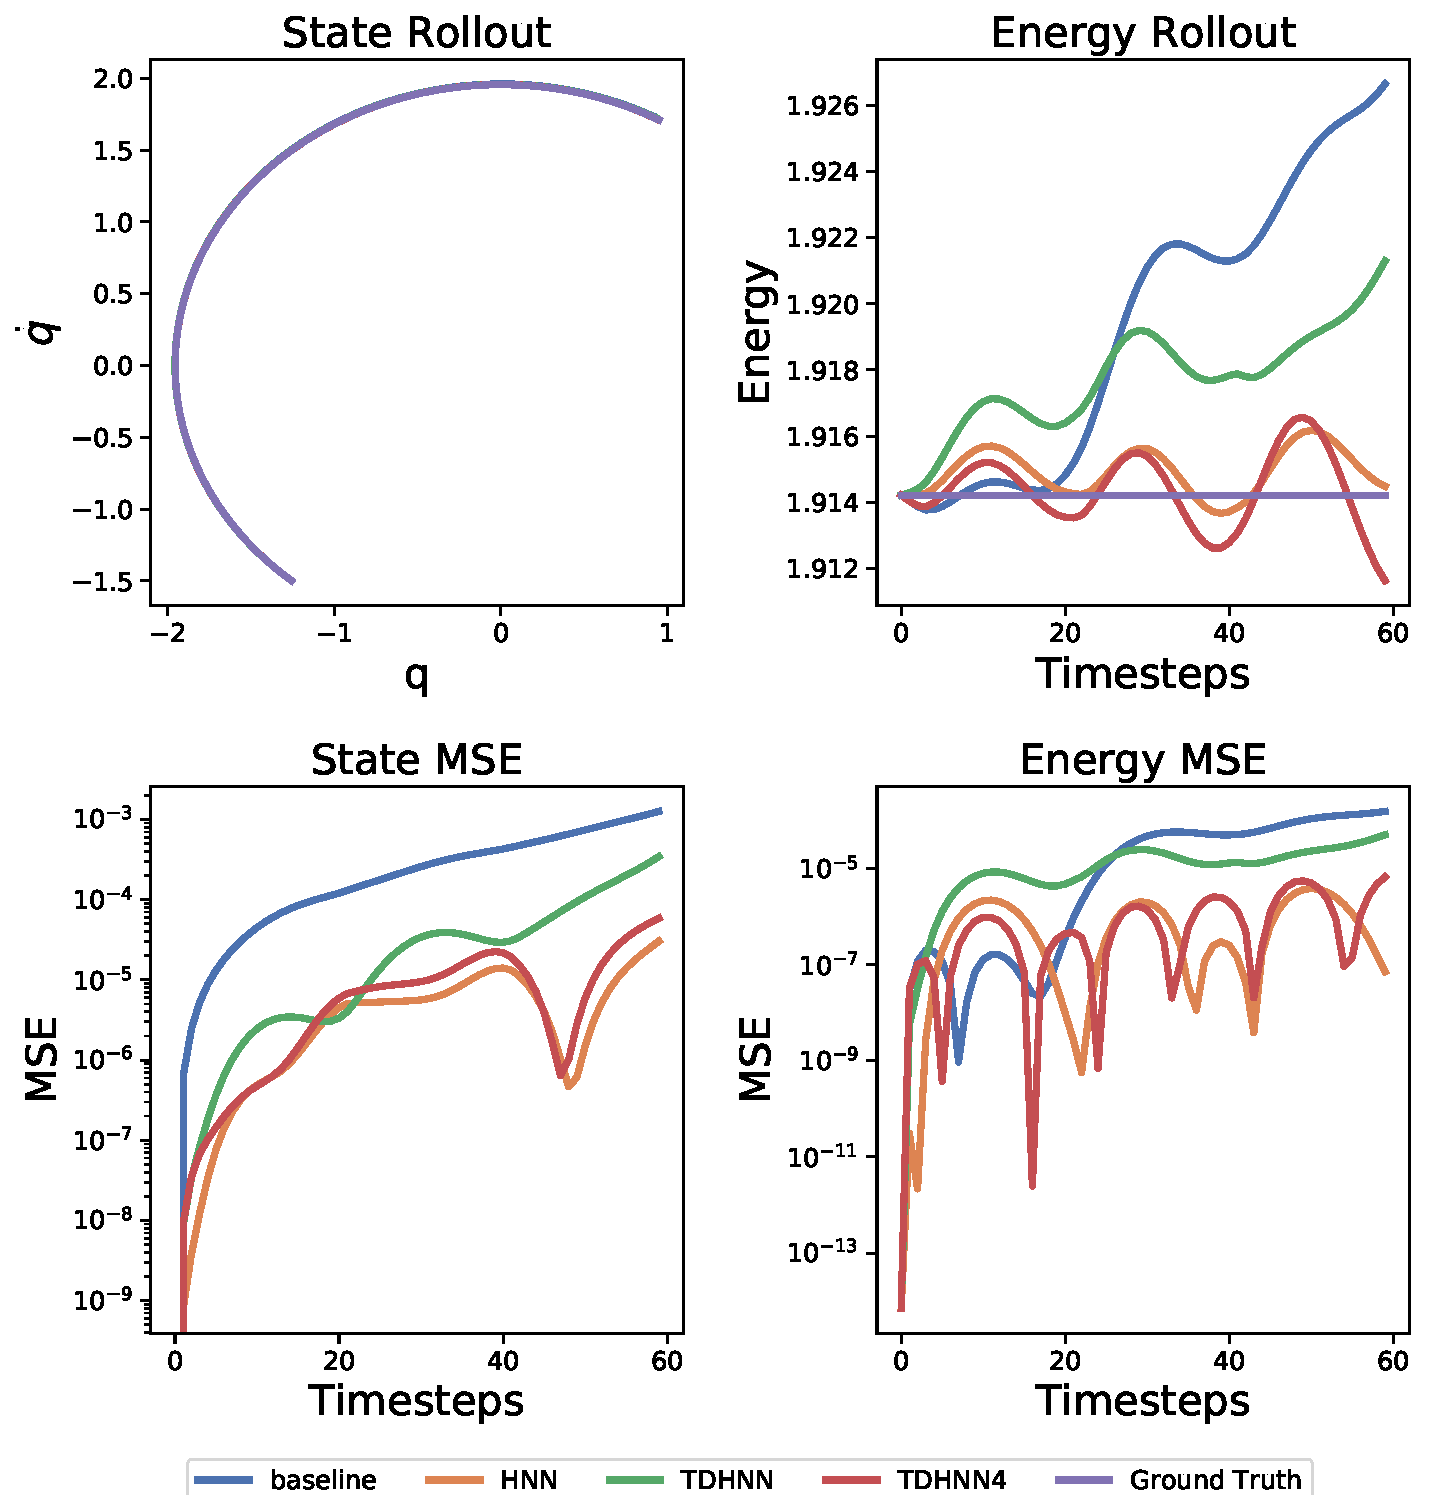
\includegraphics[width=\textwidth]{figures/figures/mass_spring/1/mass_spring_long_0.pdf}
\caption{State and energy rollout of an initial condition from the test set}
\end{subfigure}
\begin{subfigure}[b]{0.48\textwidth}
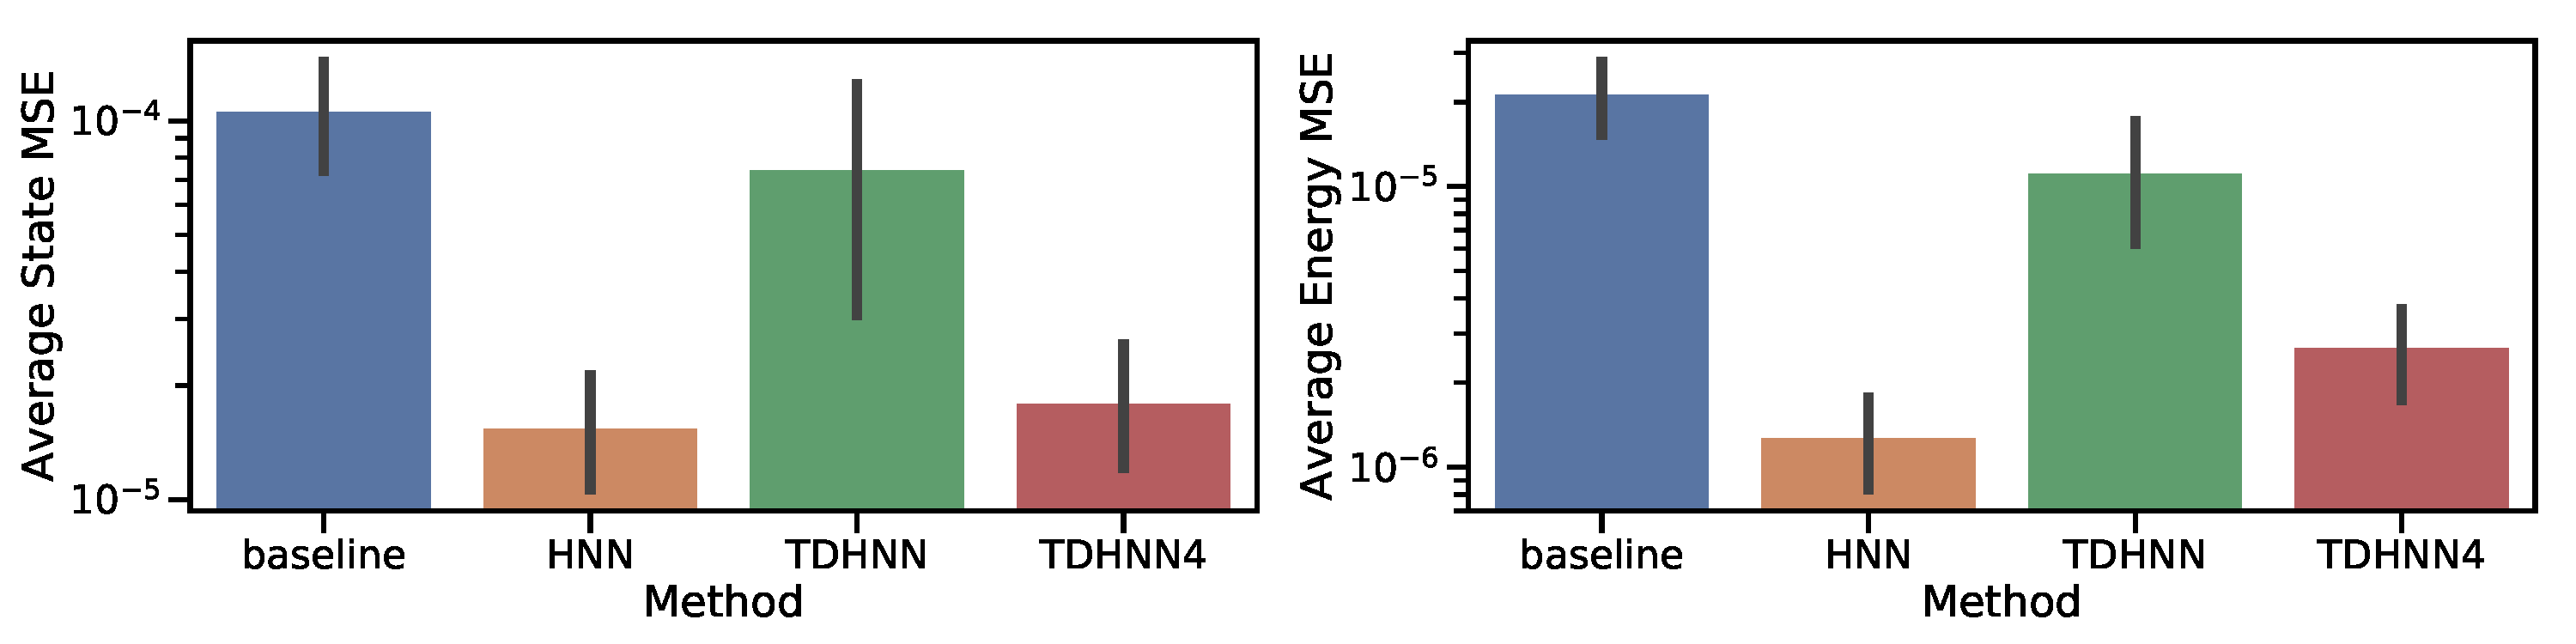
\includegraphics[width=\textwidth]{figures/figures/mass_spring/1/mass_spring_errors_0.pdf}
\caption{The average state and energy MSE across 25 test points}
\end{subfigure}
\begin{subfigure}[b]{0.48\textwidth}
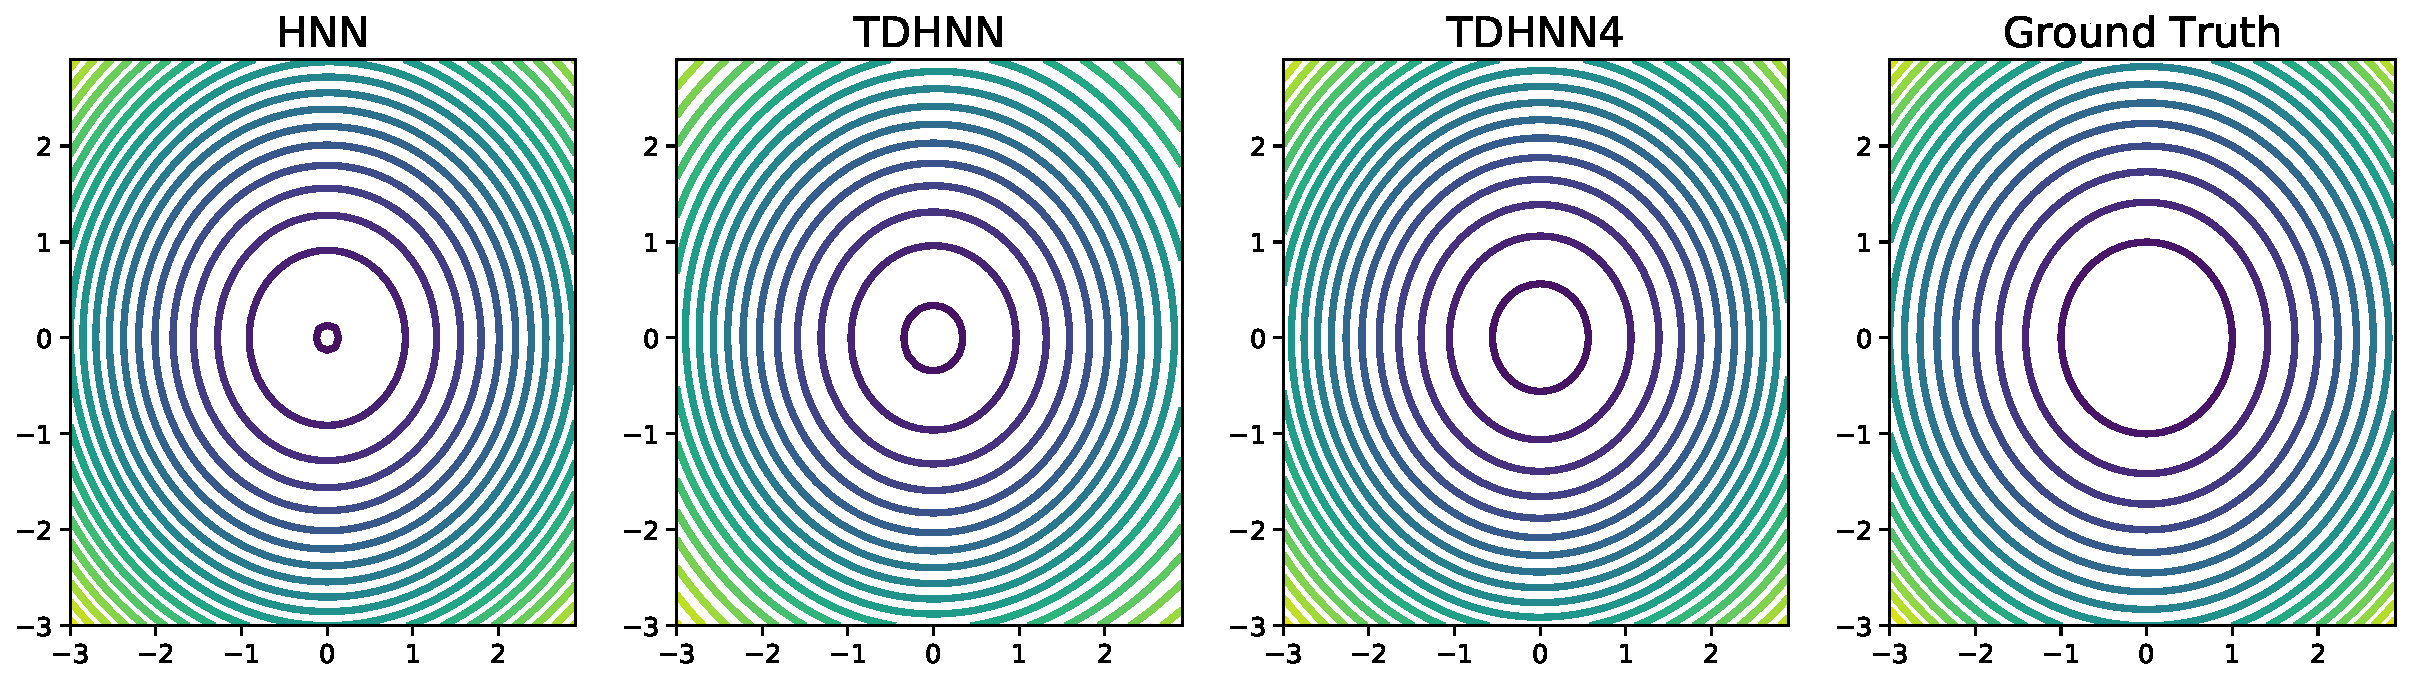
\includegraphics[width=\textwidth]{figures/figures/mass_spring/1/mass_spring_hamiltonian_0.pdf}
\caption{The learnt Hamiltonian across methods}
\end{subfigure}
\begin{subfigure}[b]{0.48\textwidth}
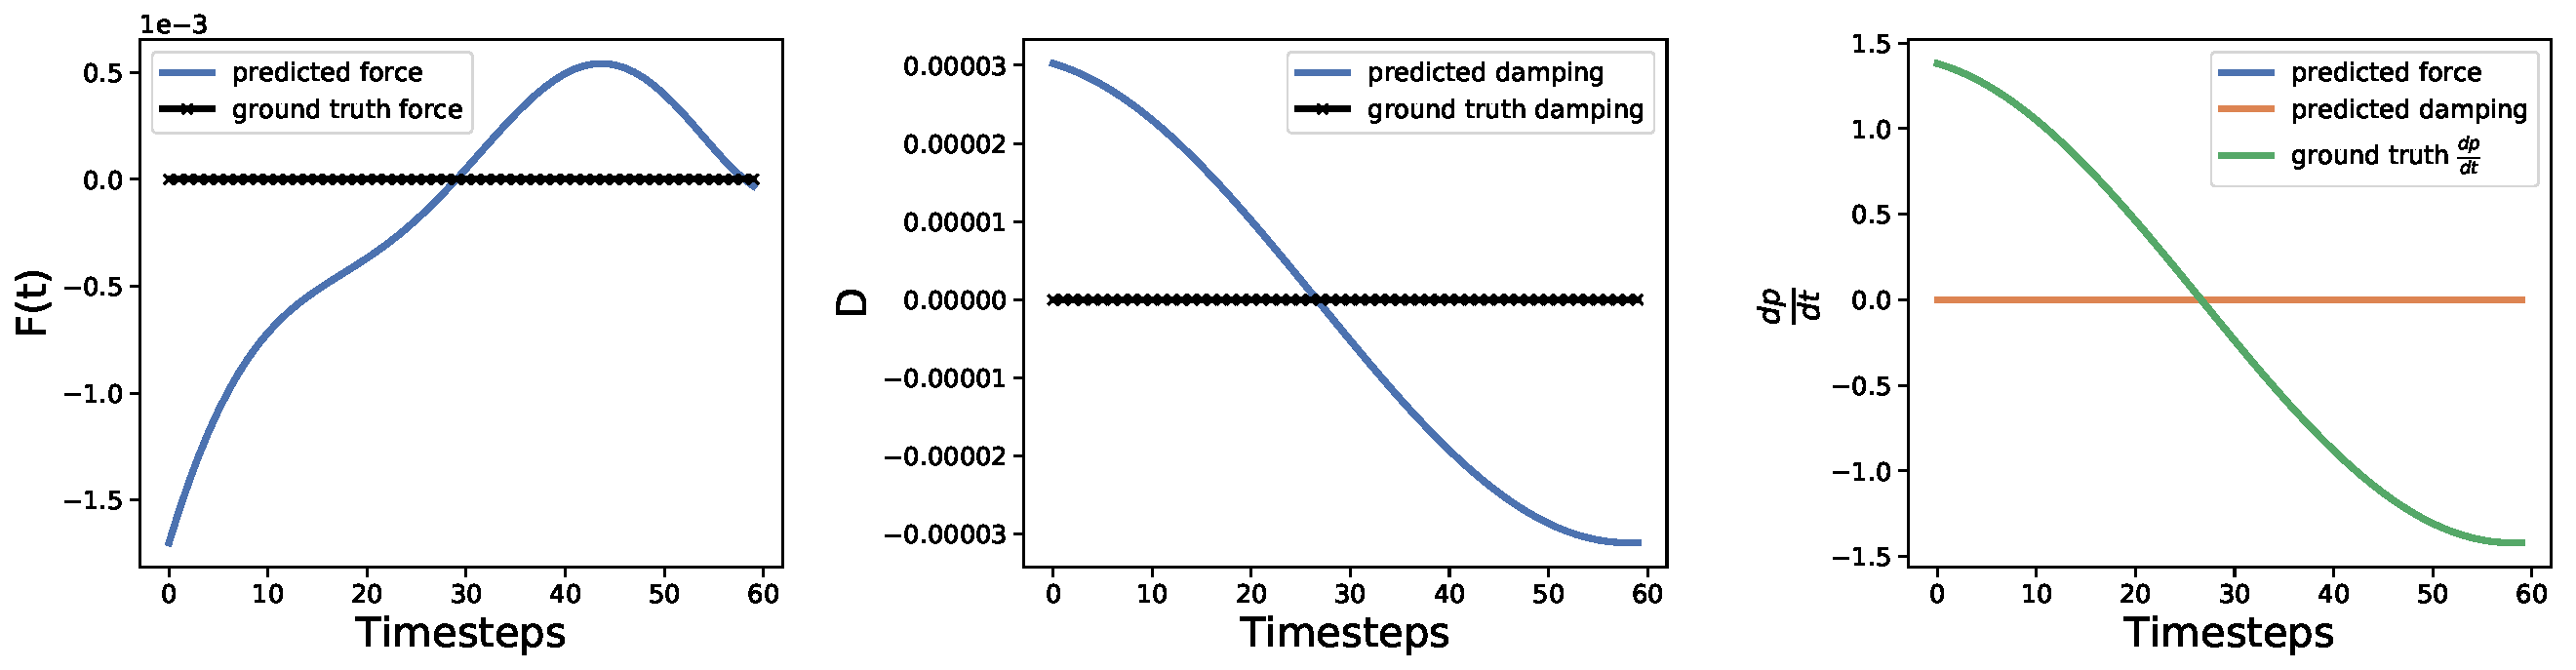
\includegraphics[width=\textwidth]{figures/figures/mass_spring/1/mass_spring_dpdt_0.pdf}
\caption{The learnt force and damping of TDHNN4}
\end{subfigure}
\label{mspring_full}
\end{figure}
\begin{figure}[!htb]
\centering
\captionsetup{justification=centering}
\begin{subfigure}[b]{0.48\textwidth}
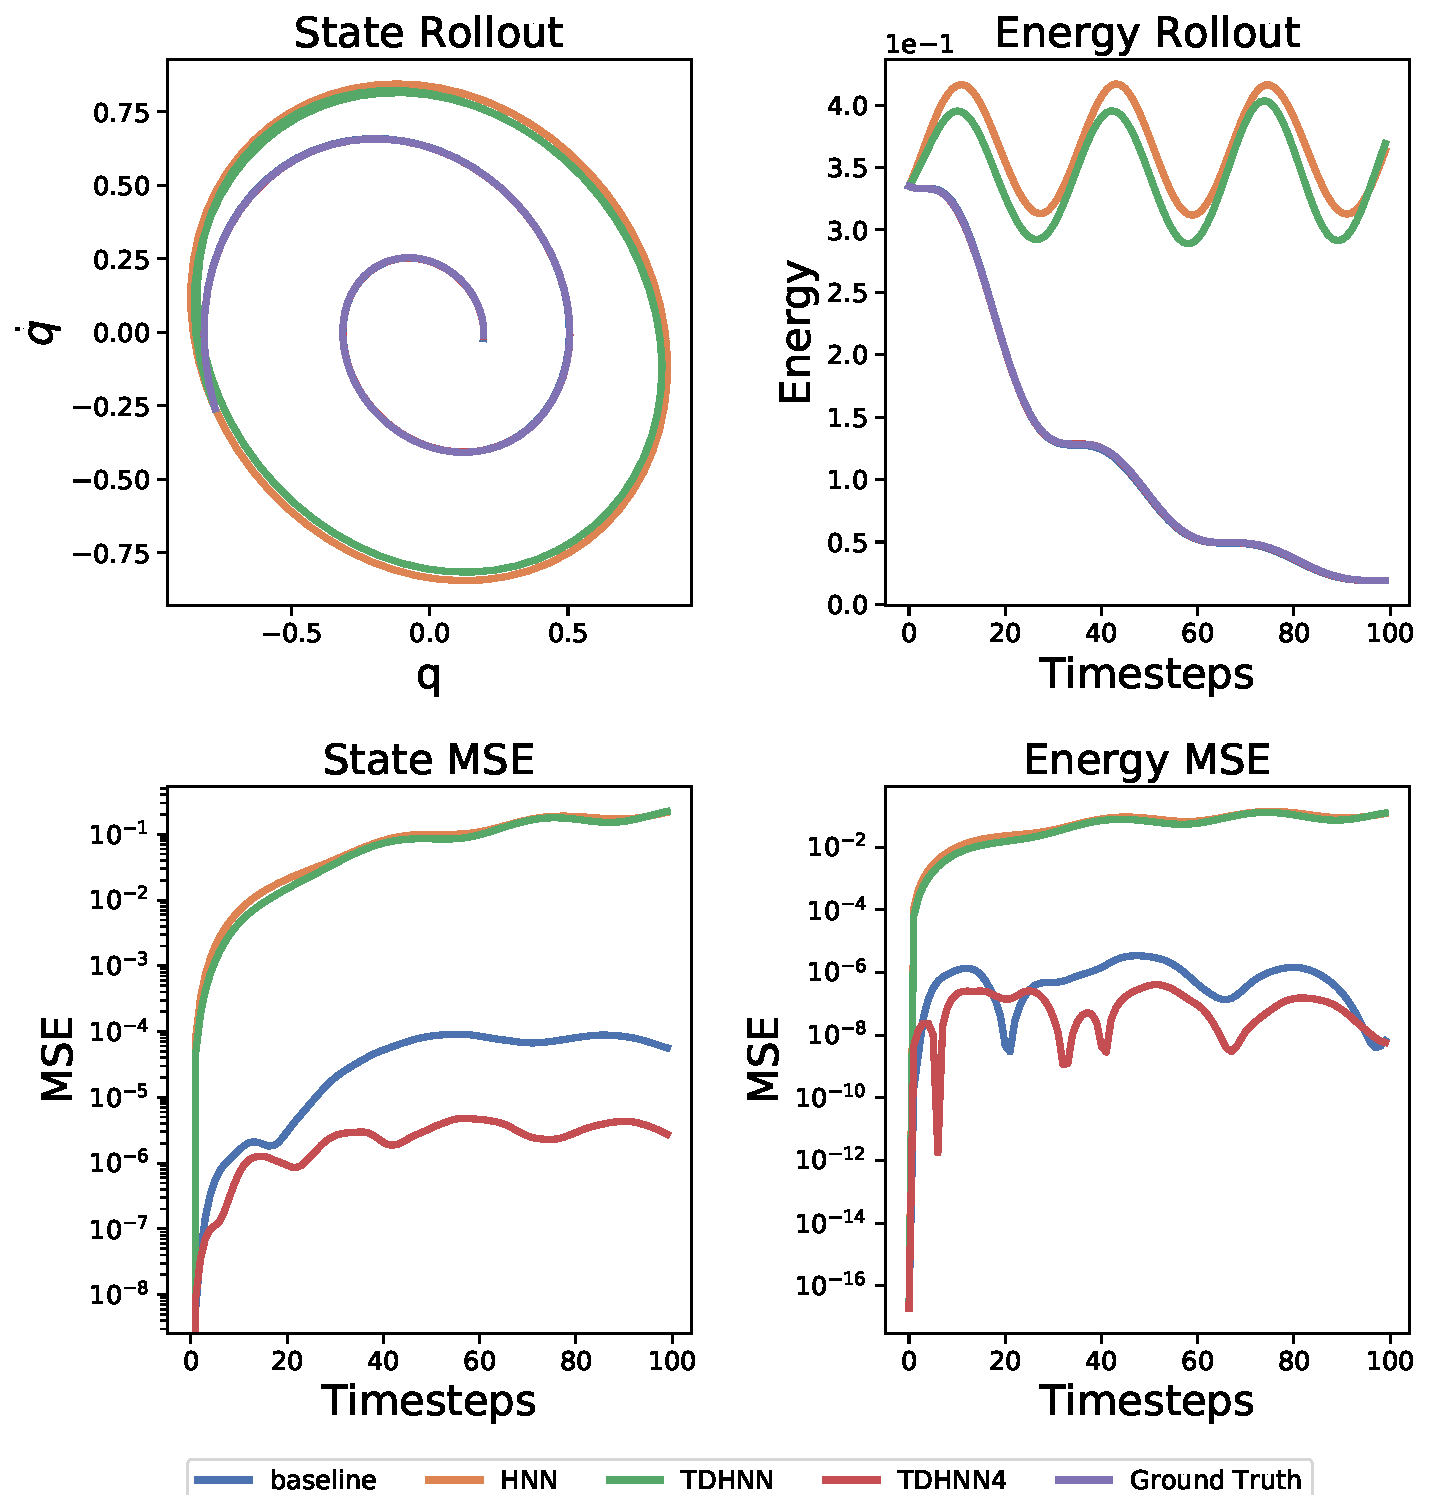
\includegraphics[width=\textwidth]{figures/figures/damped/1/damped_long_0.pdf}
\caption{State and energy rollout of an initial condition from the test set}
\end{subfigure}
\begin{subfigure}[b]{0.48\textwidth}
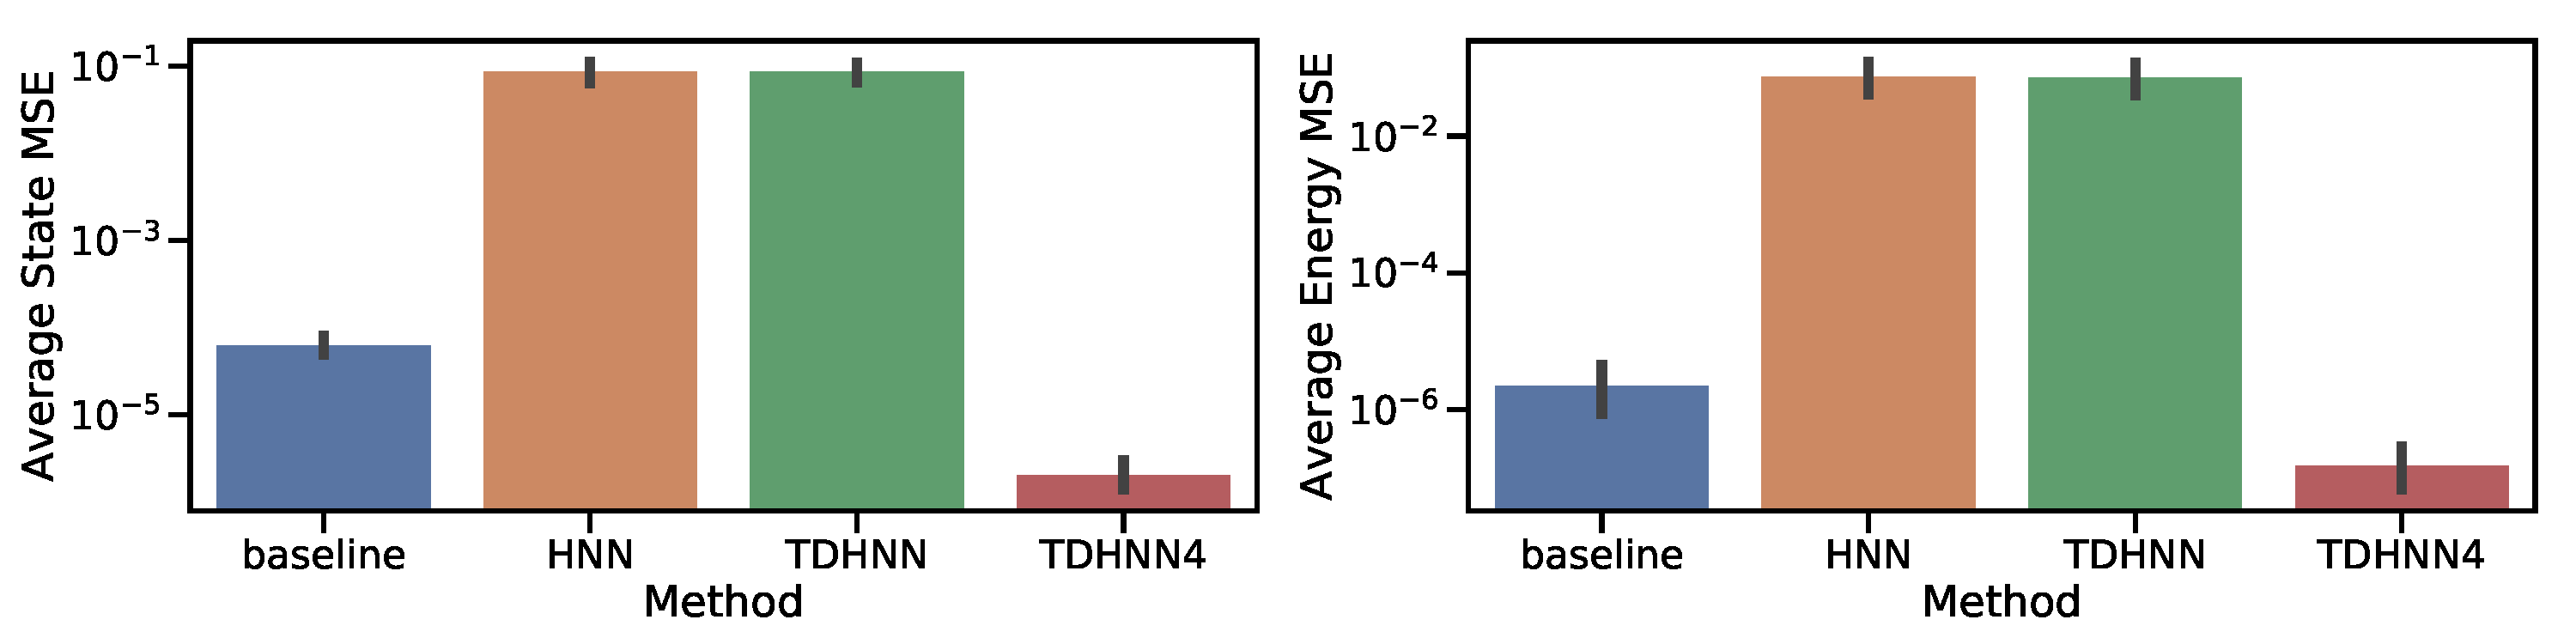
\includegraphics[width=\textwidth]{figures/figures/damped/1/damped_errors_0.pdf}
\caption{The average state and energy MSE across 25 test points}
\end{subfigure}
\begin{subfigure}[b]{0.48\textwidth}
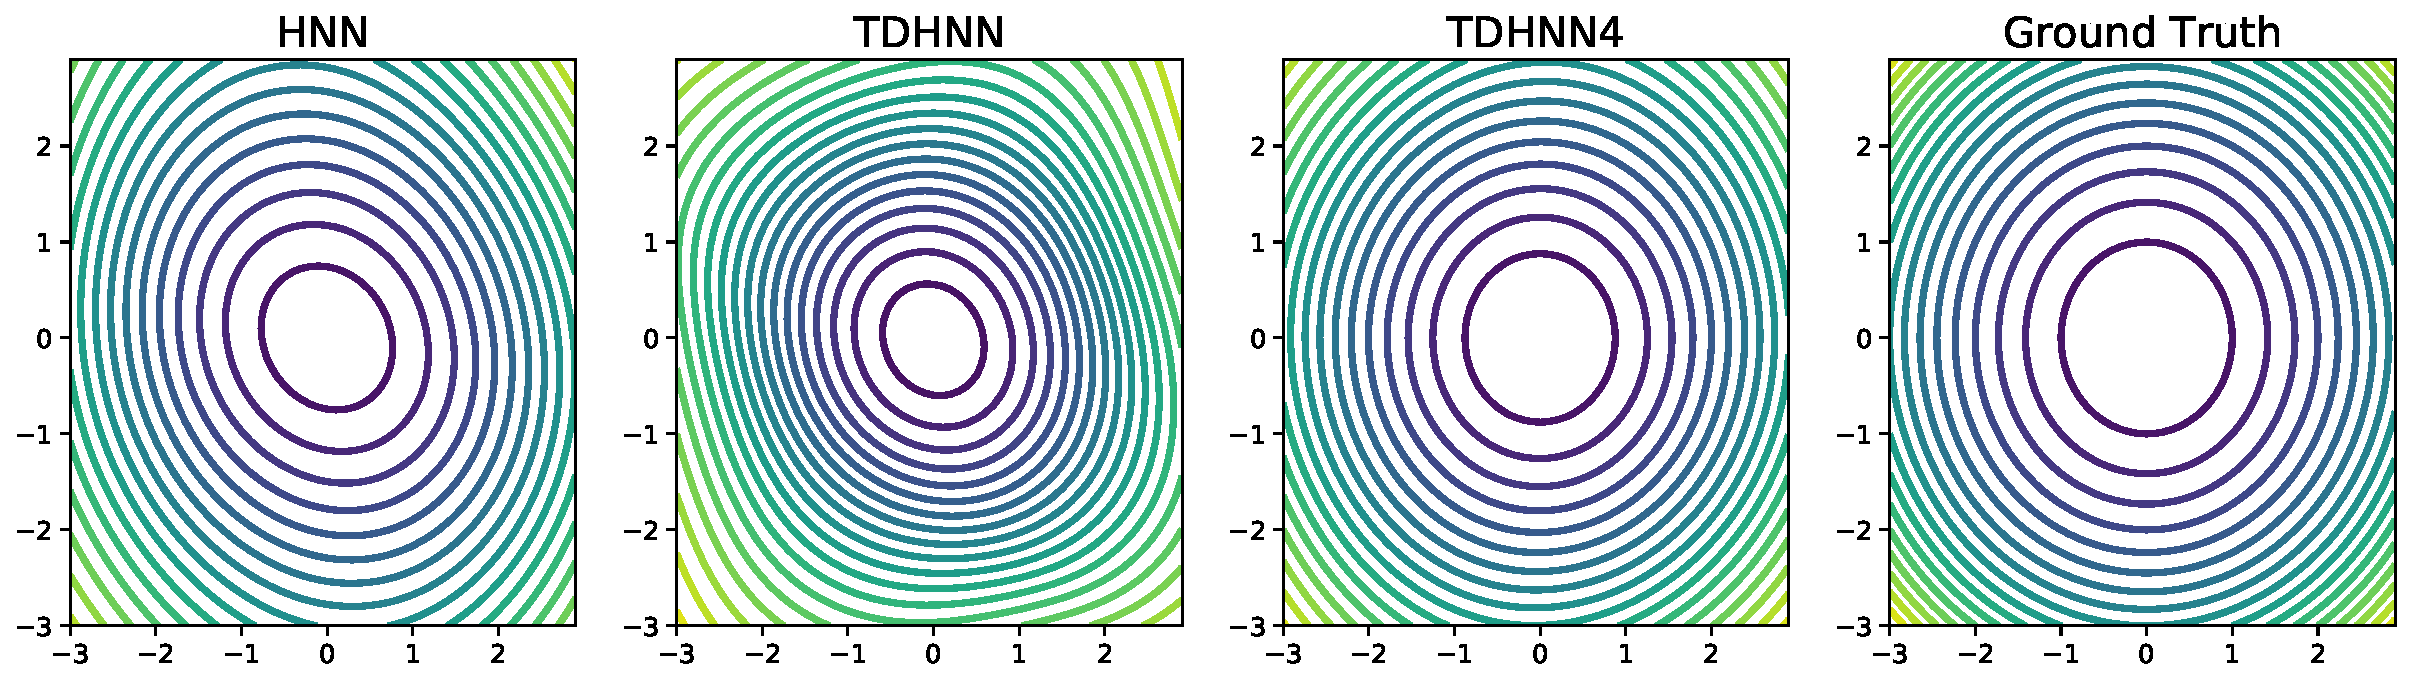
\includegraphics[width=\textwidth]{figures/figures/damped/1/damped_hamiltonian_0.pdf}
\caption{The learnt Hamiltonian across methods}
\end{subfigure}
\begin{subfigure}[b]{0.48\textwidth}
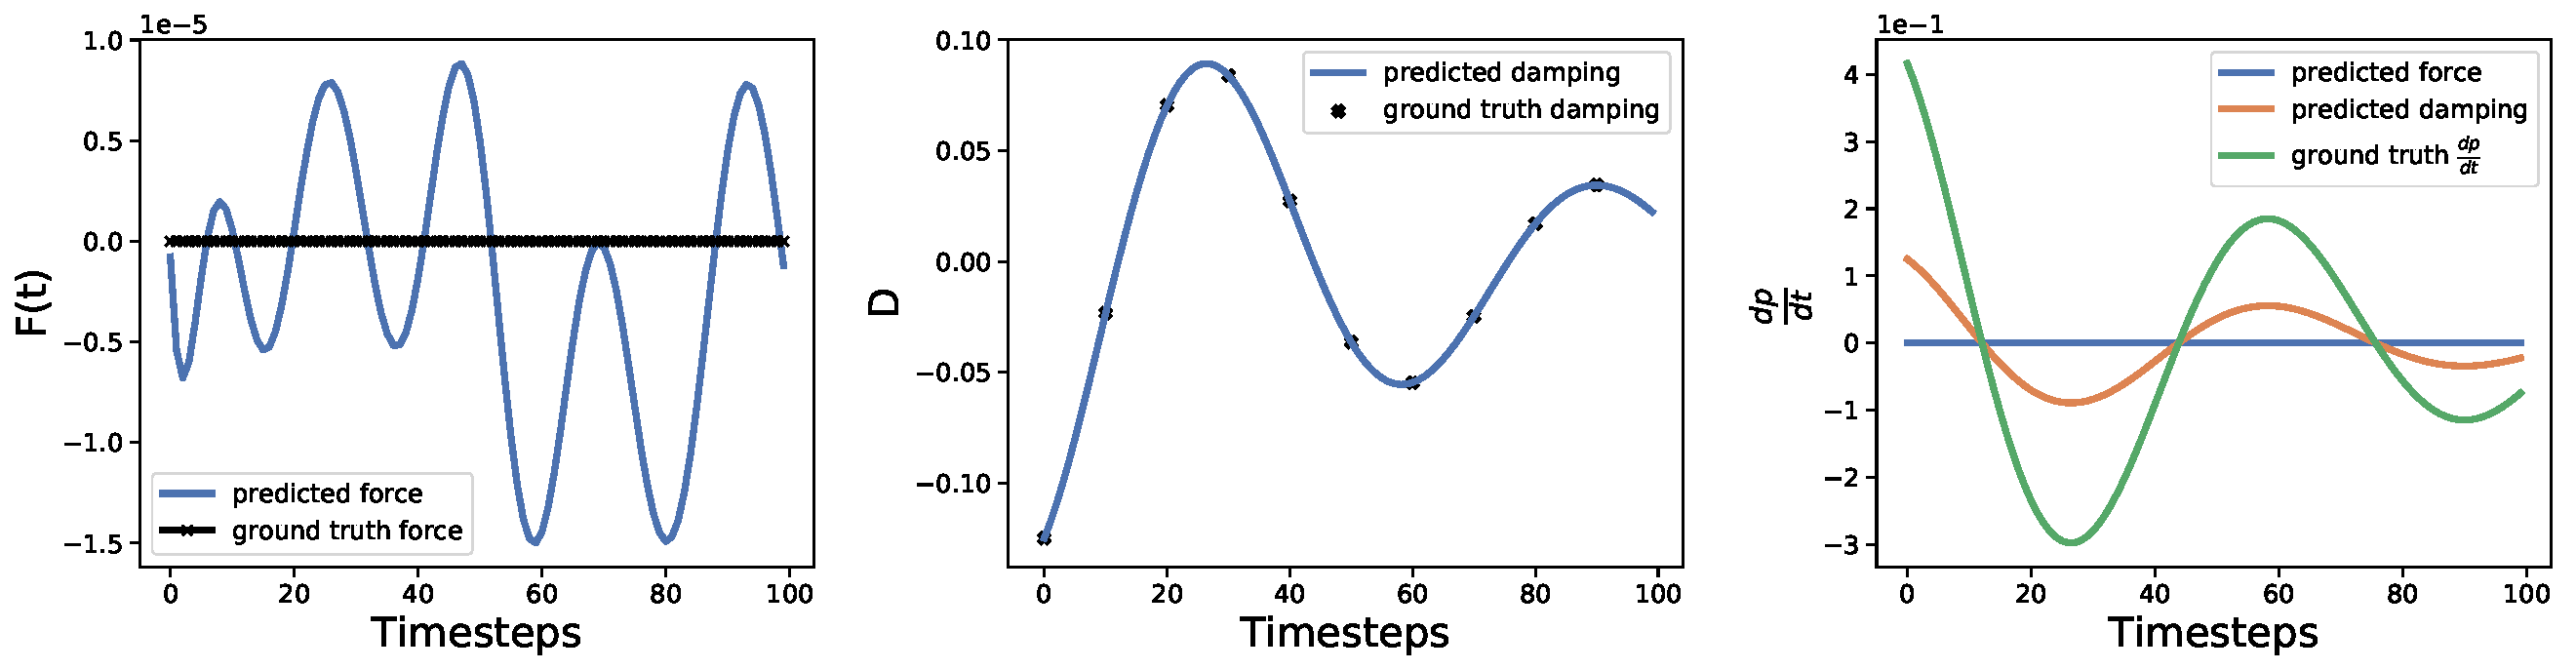
\includegraphics[width=\textwidth]{figures/figures/damped/1/damped_dpdt_0.pdf}
\caption{The learnt force and damping of TDHNN4}
\end{subfigure}
\label{mspring_full}
\end{figure}
\begin{figure}[!htb]
\centering
\captionsetup{justification=centering}
\begin{subfigure}[b]{0.48\textwidth}
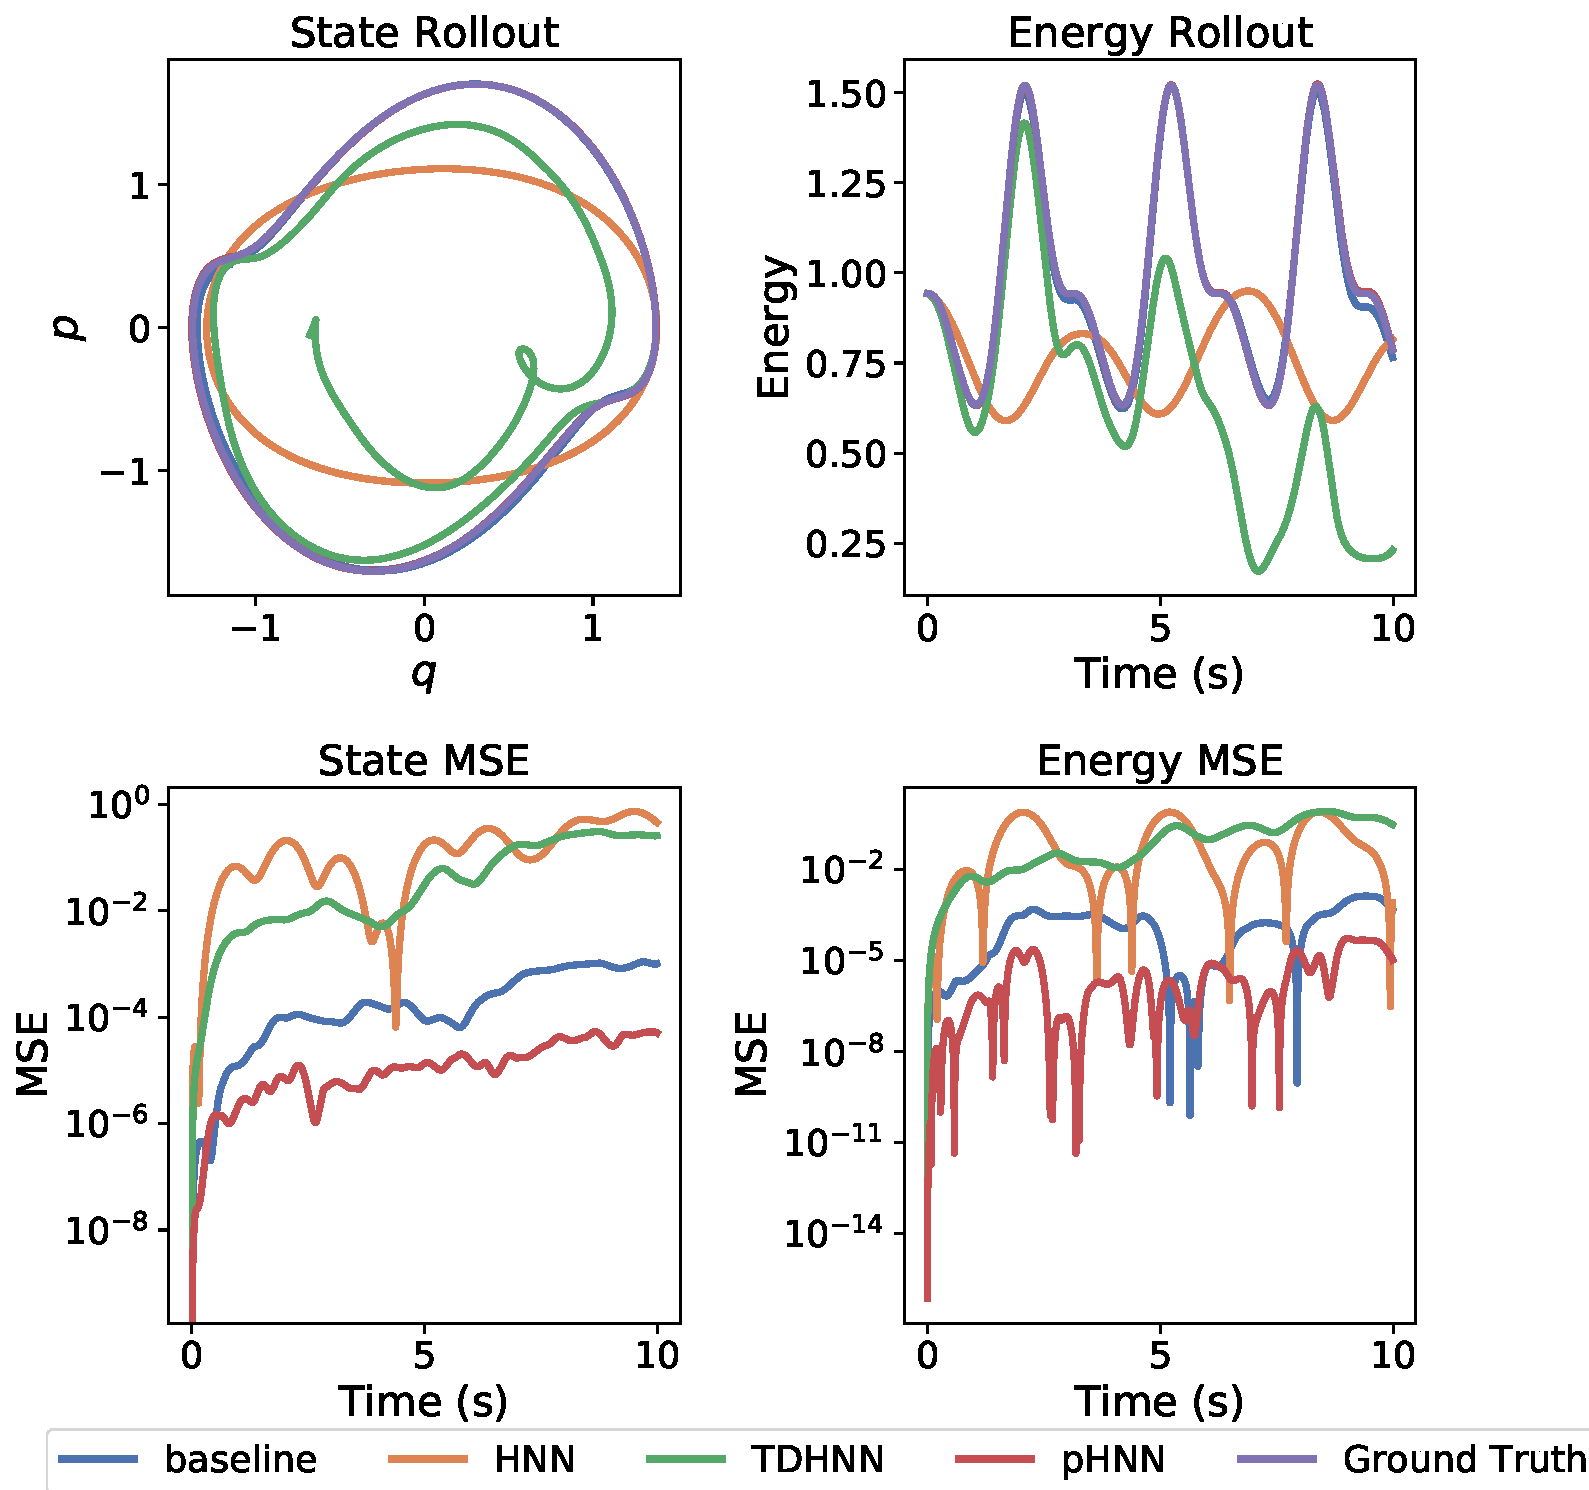
\includegraphics[width=\textwidth]{figures/figures/forced_mass_spring/1/forced_mass_spring_long_0.pdf}
\caption{State and energy rollout of an initial condition from the test set}
\end{subfigure}
\begin{subfigure}[b]{0.48\textwidth}
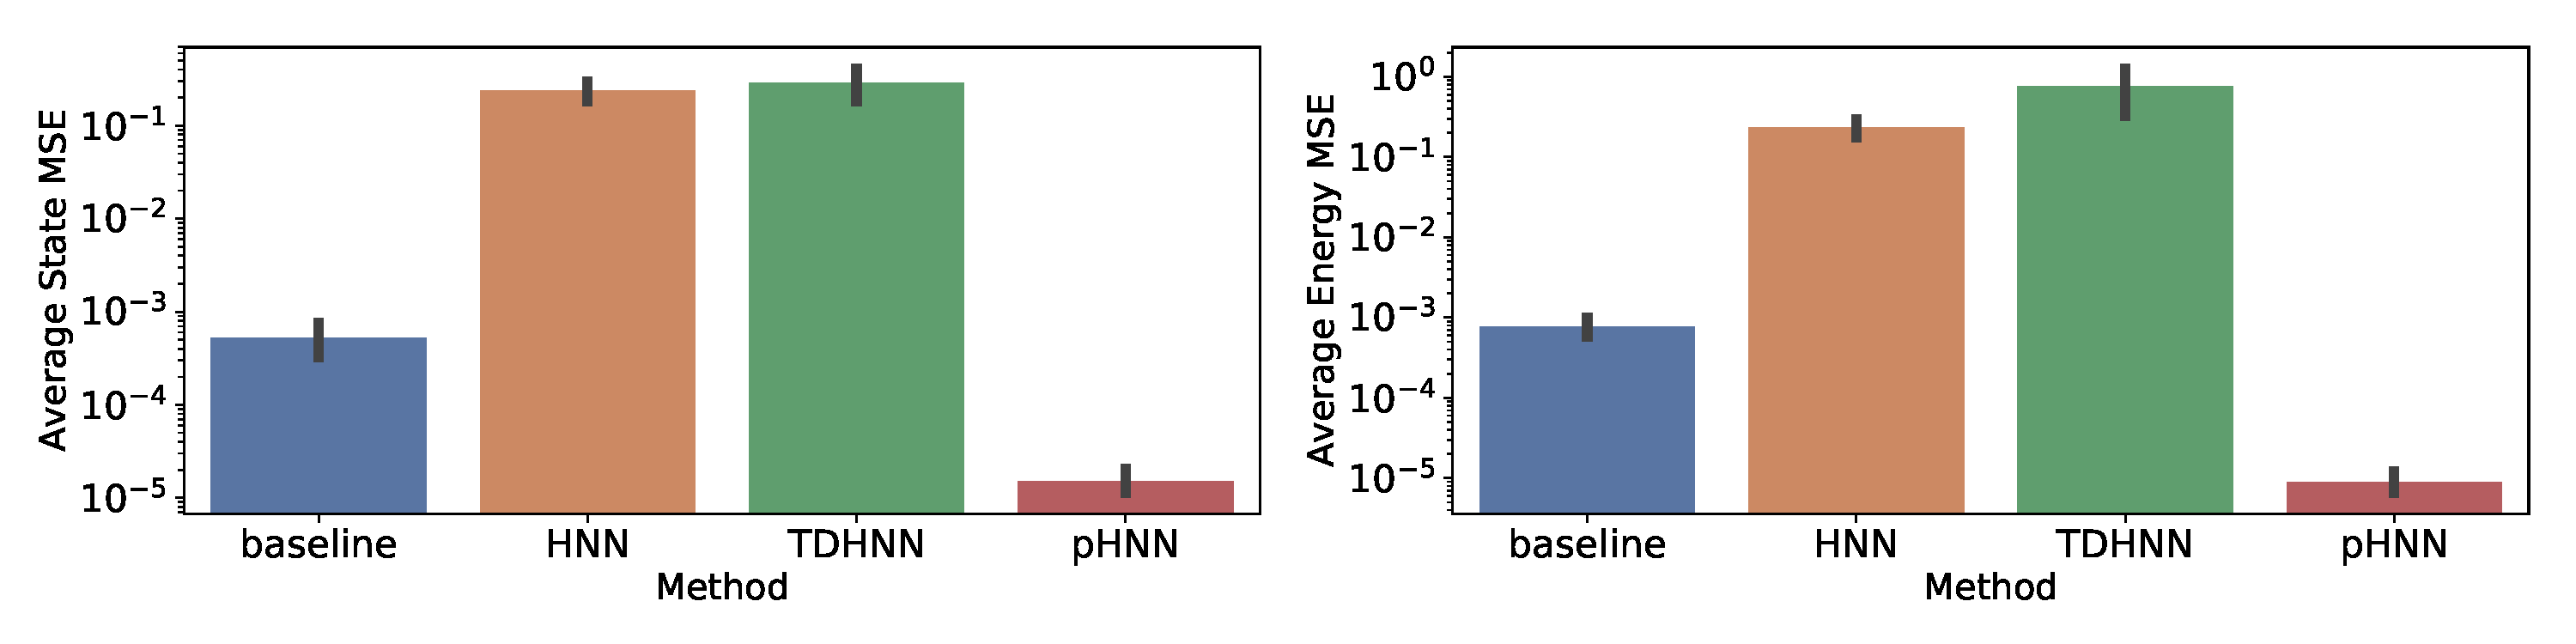
\includegraphics[width=\textwidth]{figures/figures/forced_mass_spring/1/forced_mass_spring_errors_0.pdf}
\caption{The average state and energy MSE across 25 test points}
\end{subfigure}
\begin{subfigure}[b]{0.48\textwidth}
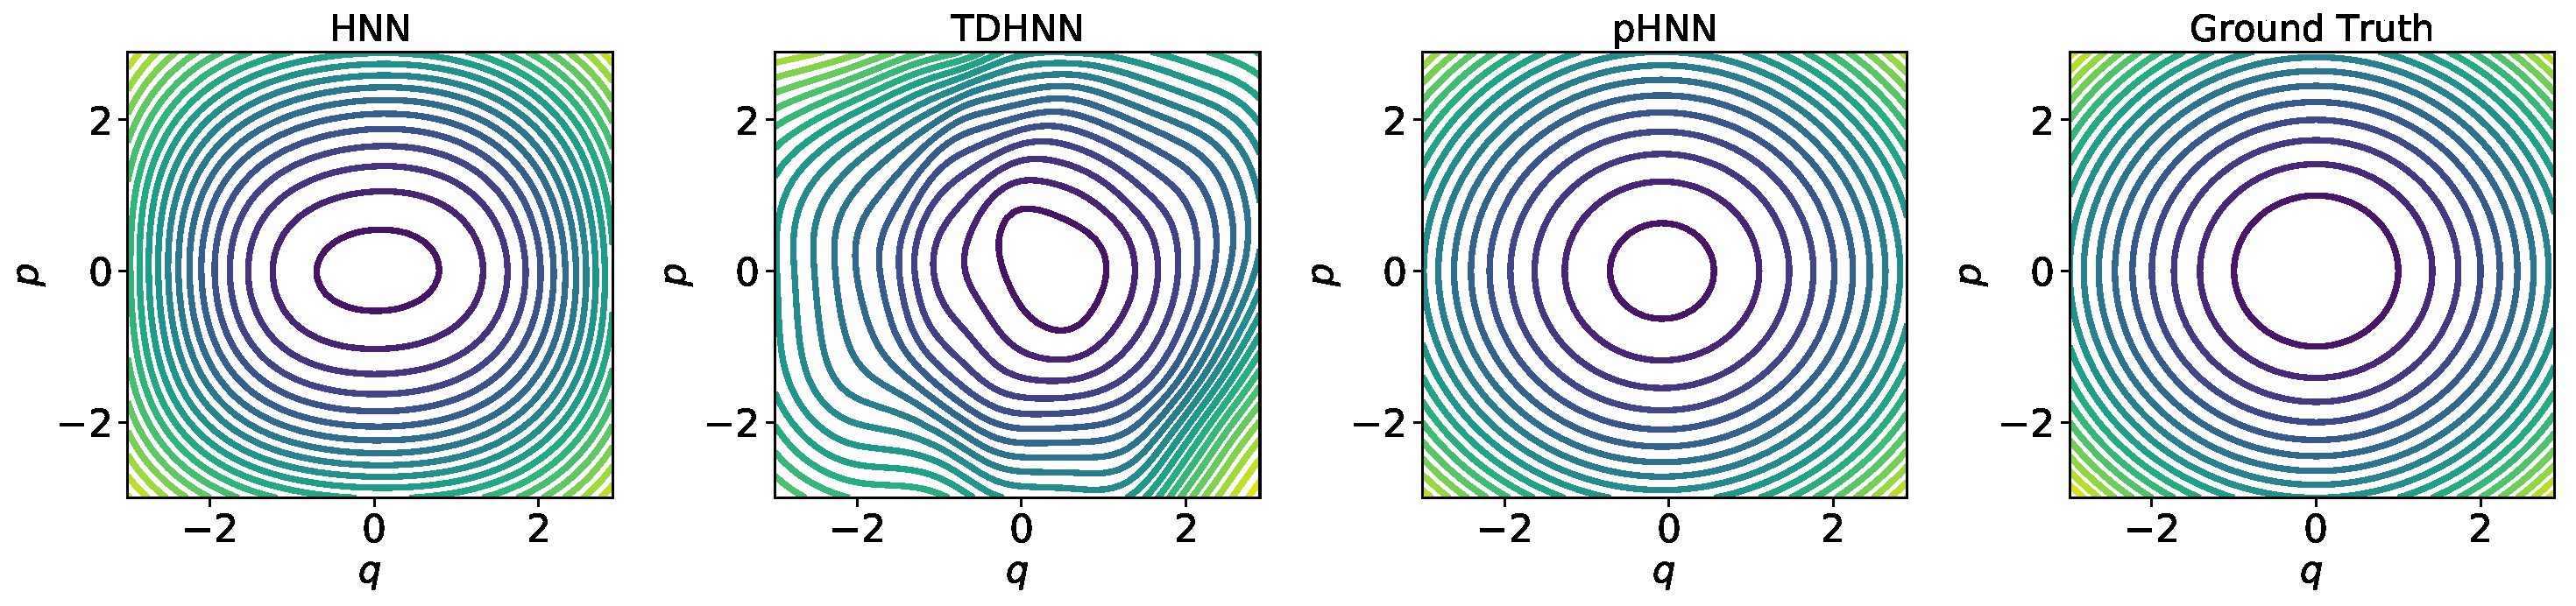
\includegraphics[width=\textwidth]{figures/figures/forced_mass_spring/1/forced_mass_spring_hamiltonian_0.pdf}
\caption{The learnt Hamiltonian across methods}
\end{subfigure}
\begin{subfigure}[b]{0.48\textwidth}
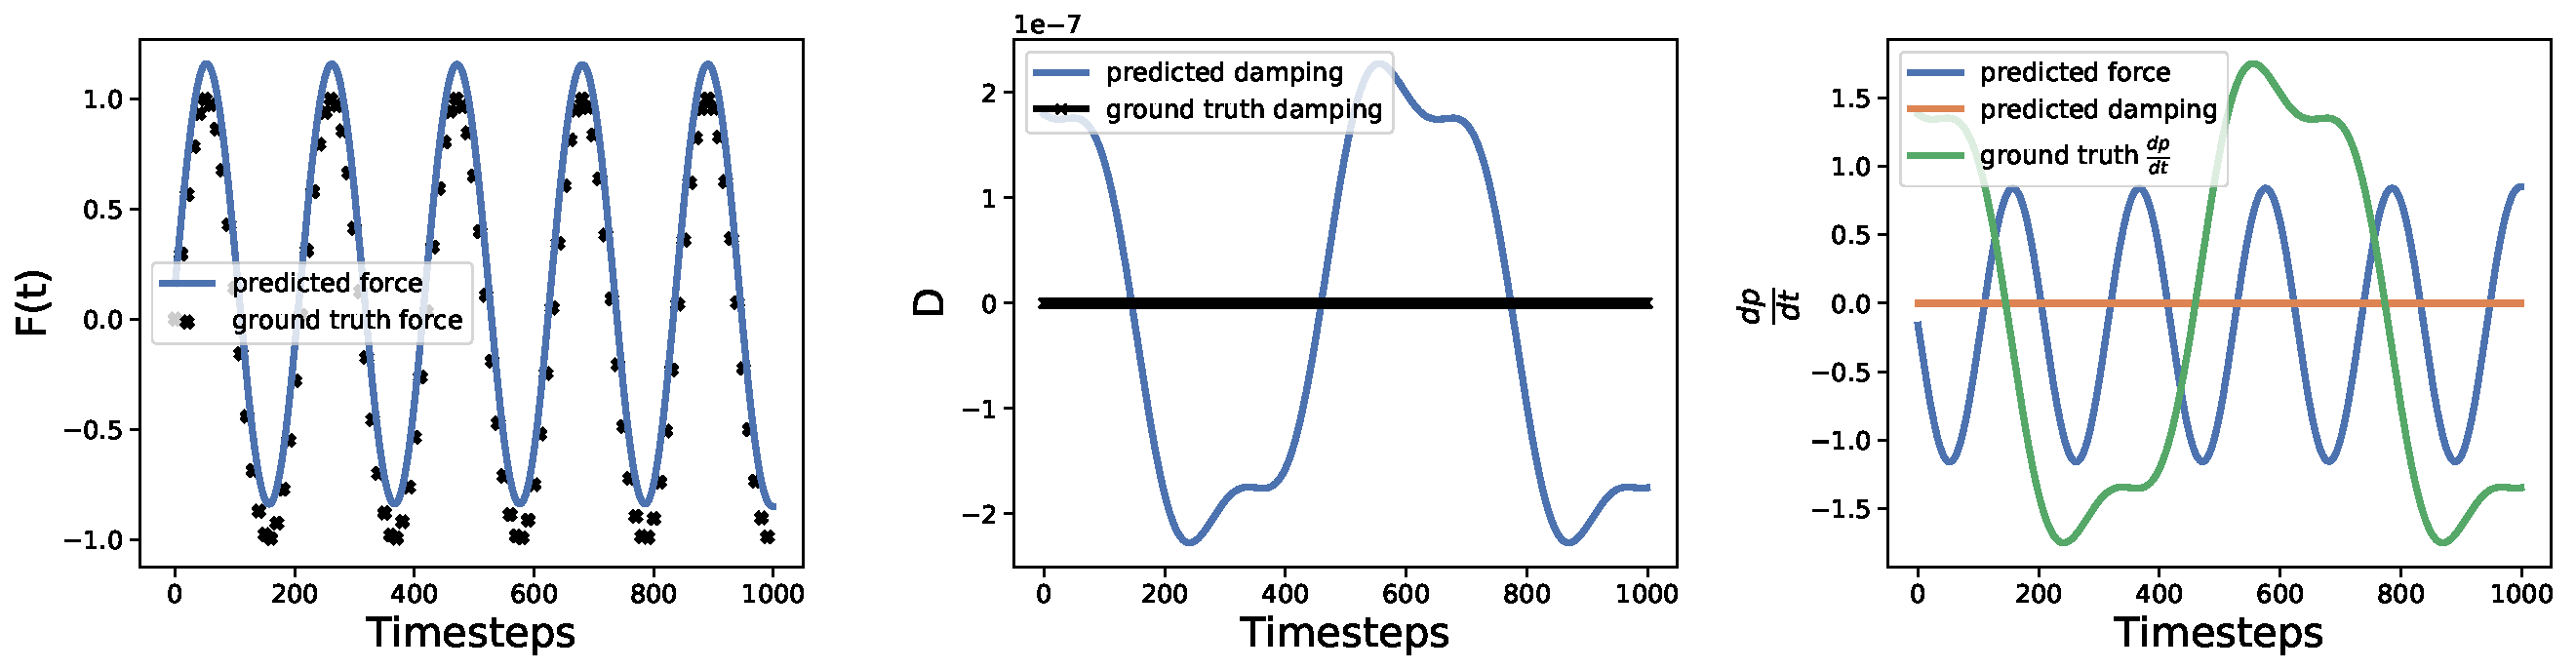
\includegraphics[width=\textwidth]{figures/figures/forced_mass_spring/1/forced_mass_spring_dpdt_0.pdf}
\caption{The learnt force and damping of TDHNN4}
\end{subfigure}
\label{forced_mspring_1_full}
\end{figure}
\begin{figure}[!htb]
\centering
\captionsetup{justification=centering}
\begin{subfigure}[b]{0.48\textwidth}
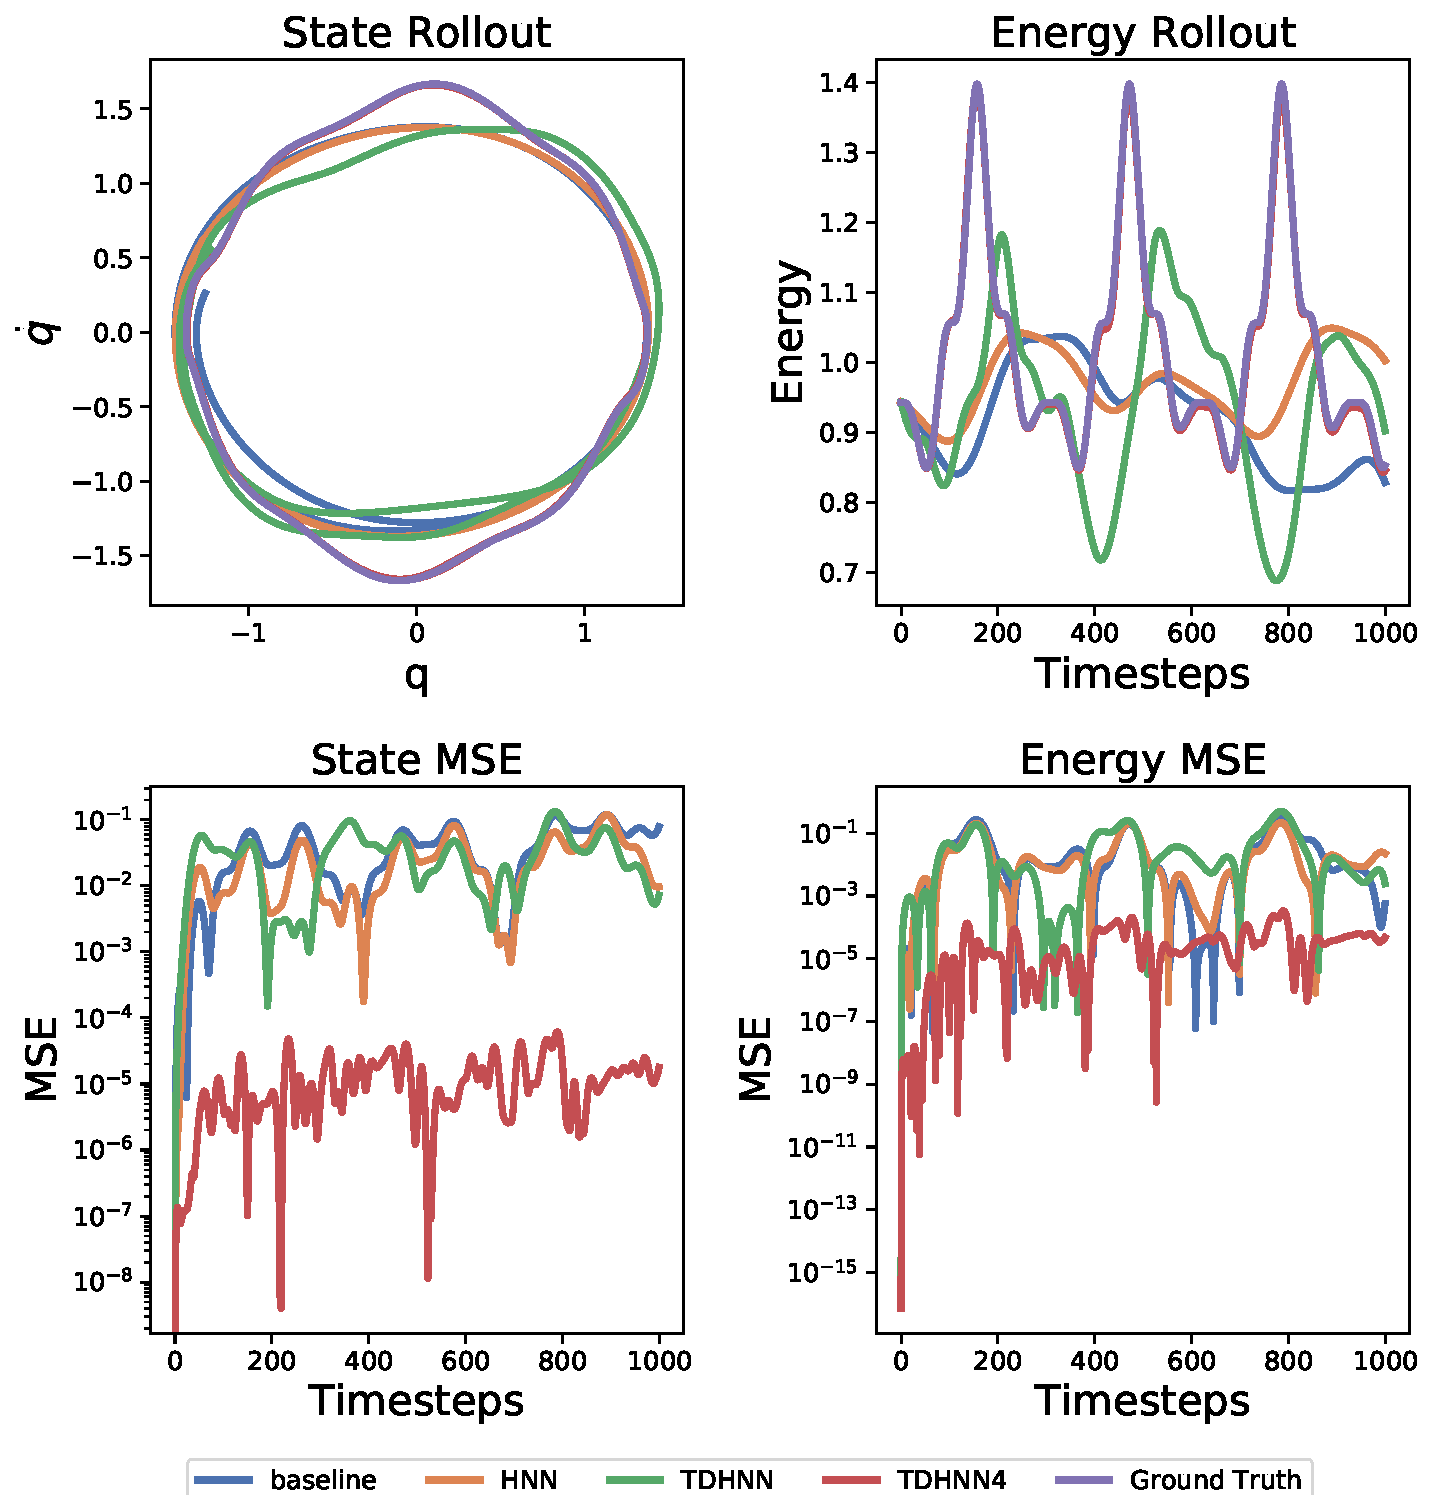
\includegraphics[width=\textwidth]{figures/figures/forced_mass_spring/2/forced_mass_spring_long_0.pdf}
\caption{State and energy rollout of an initial condition from the test set}
\end{subfigure}
\begin{subfigure}[b]{0.48\textwidth}
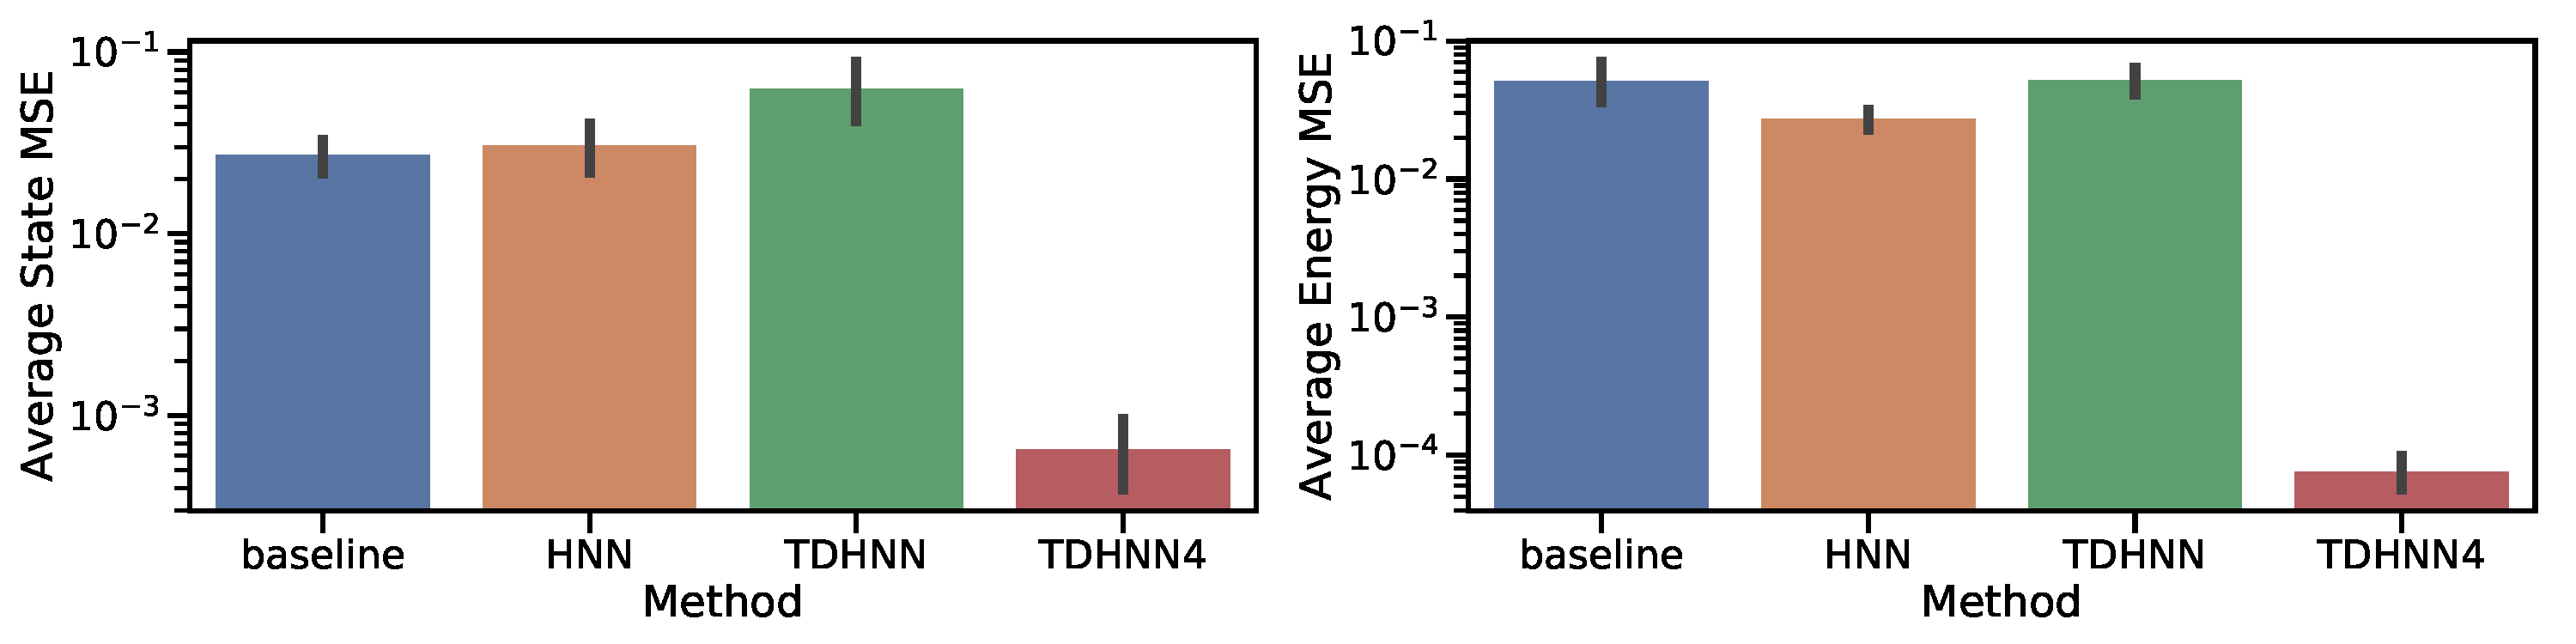
\includegraphics[width=\textwidth]{figures/figures/forced_mass_spring/2/forced_mass_spring_errors_0.pdf}
\caption{The average state and energy MSE across 25 test points}
\end{subfigure}
\begin{subfigure}[b]{0.48\textwidth}
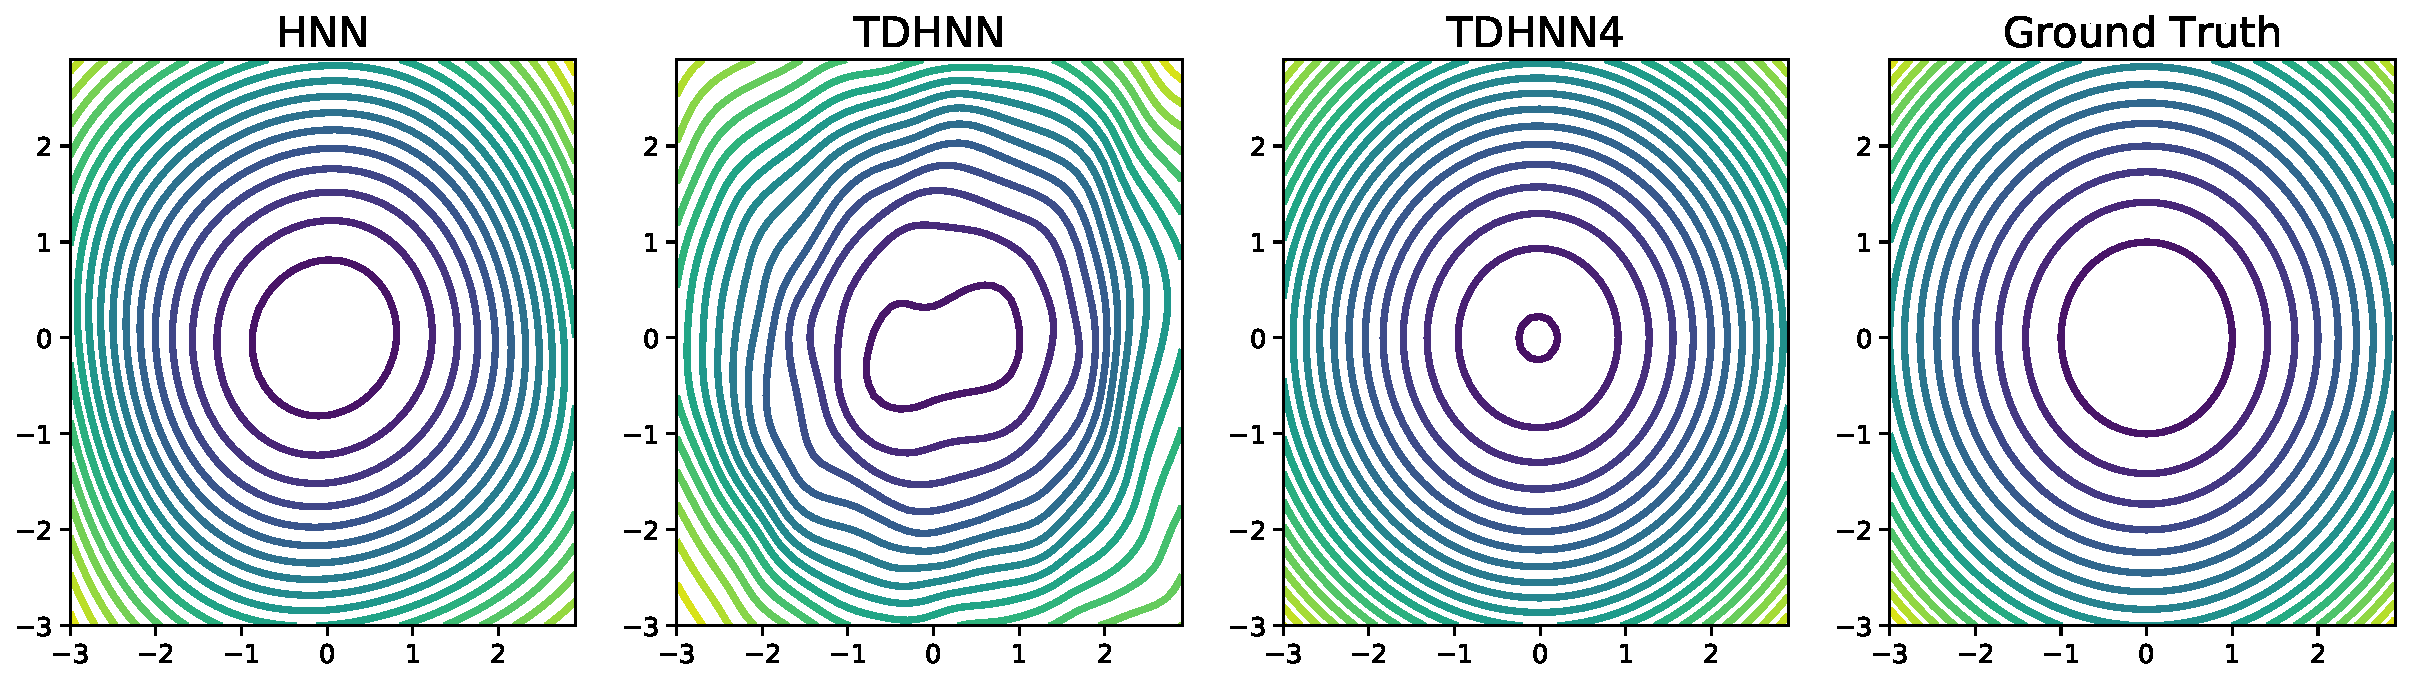
\includegraphics[width=\textwidth]{figures/figures/forced_mass_spring/2/forced_mass_spring_hamiltonian_0.pdf}
\caption{The learnt Hamiltonian across methods}
\end{subfigure}
\begin{subfigure}[b]{0.48\textwidth}
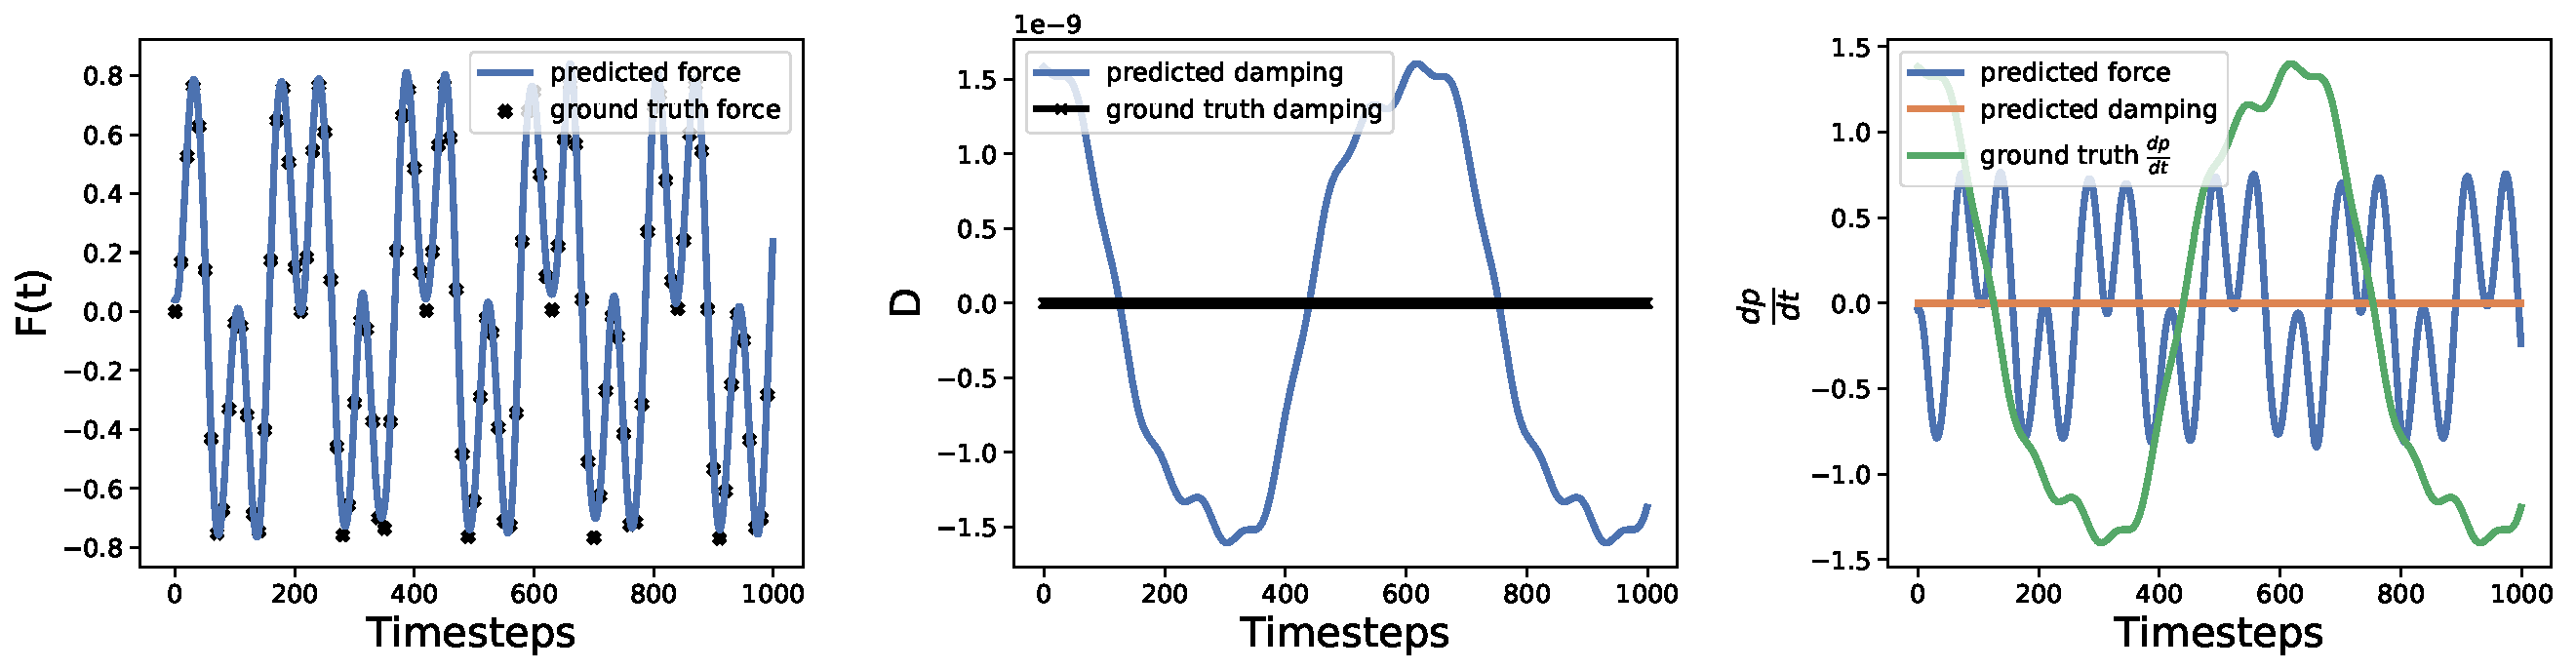
\includegraphics[width=\textwidth]{figures/figures/forced_mass_spring/2/forced_mass_spring_dpdt_0.pdf}
\caption{The learnt force and damping of TDHNN4}
\end{subfigure}
\label{forced_mpsring_2_full}
\end{figure}
\begin{figure}[!htb]
\centering
\captionsetup{justification=centering}
\begin{subfigure}[b]{0.48\textwidth}
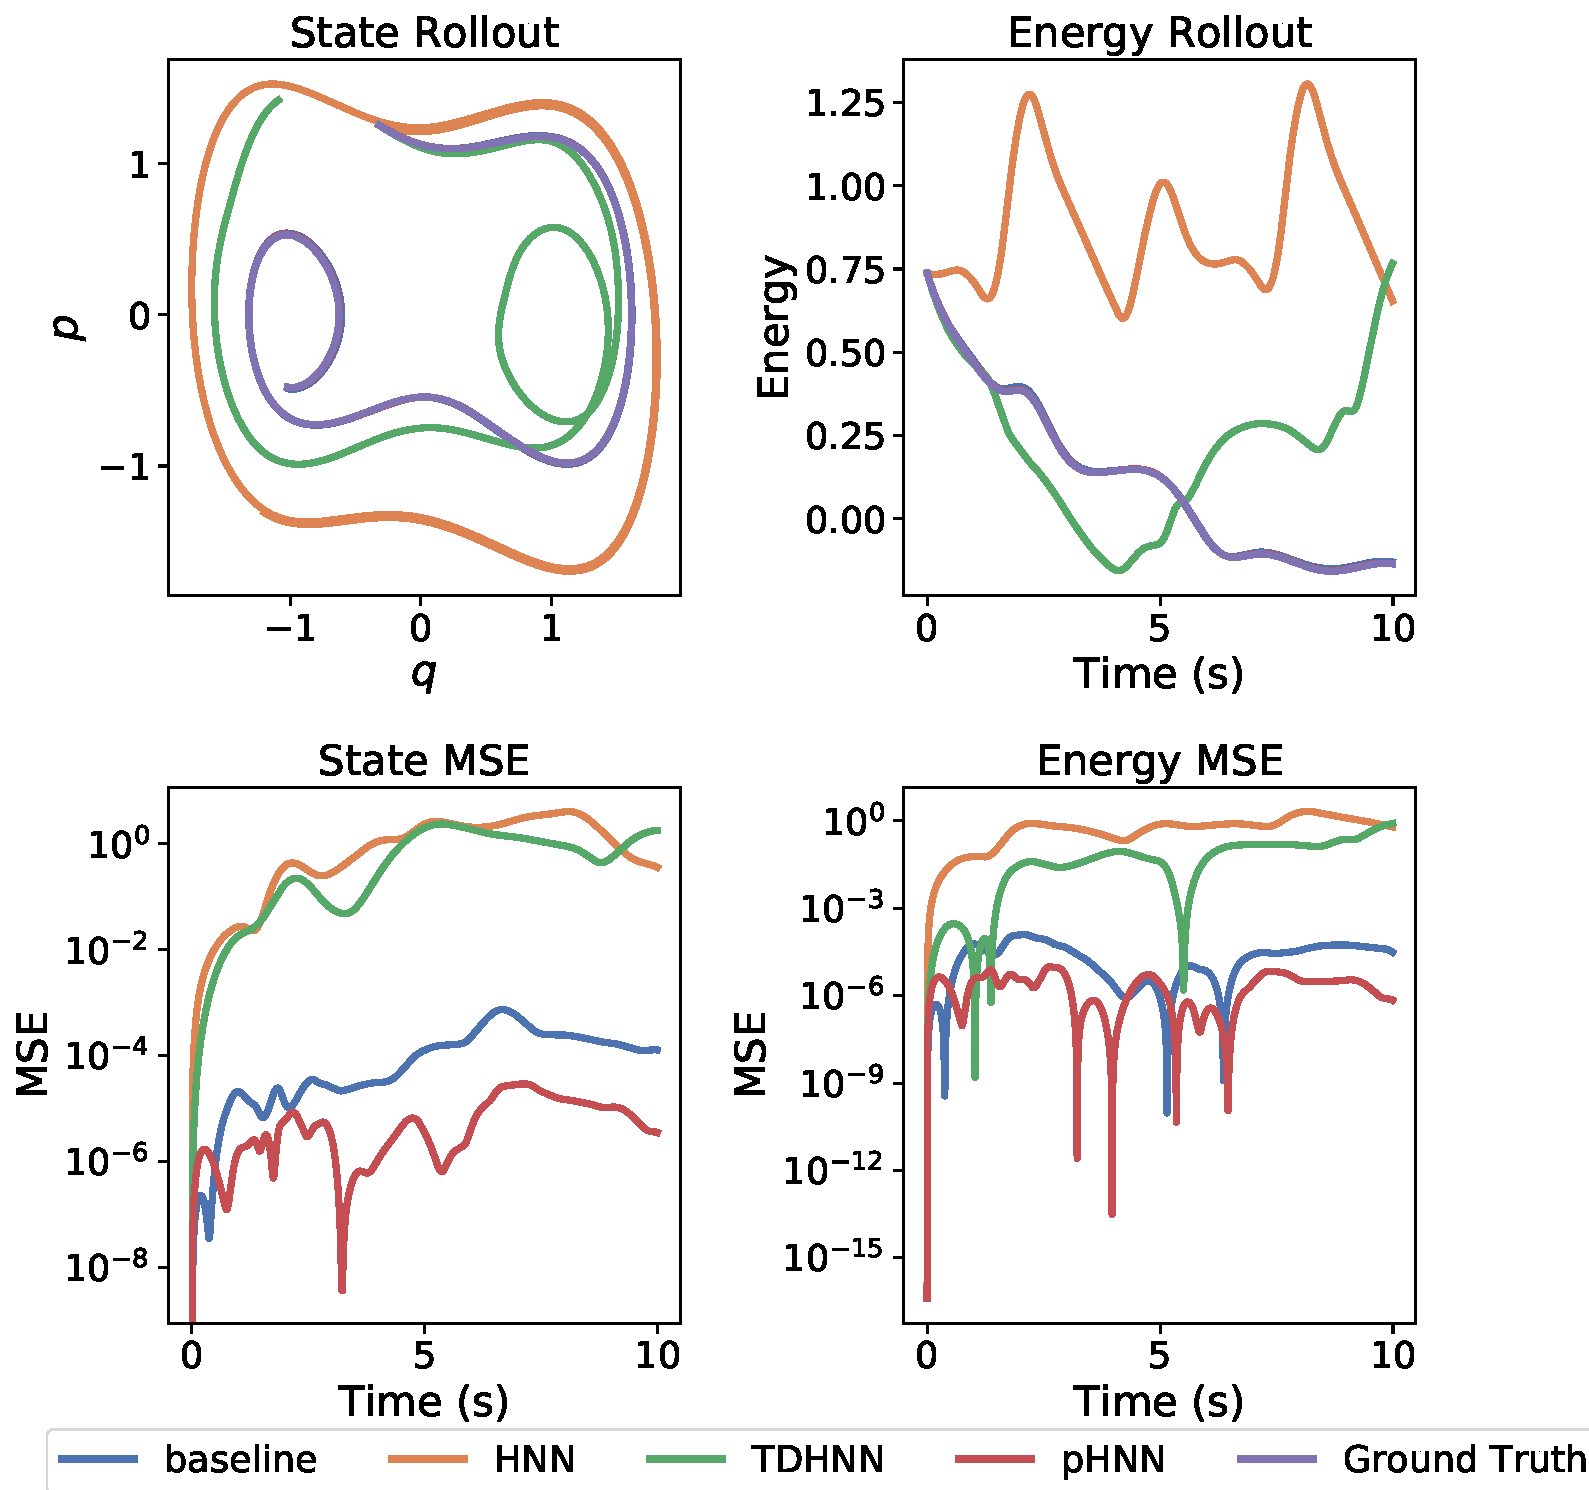
\includegraphics[width=\textwidth]{figures/figures/duffing/1/duffing_long_0.pdf}
\caption{State and energy rollout of an initial condition from the test set}
\end{subfigure}
\begin{subfigure}[b]{0.48\textwidth}
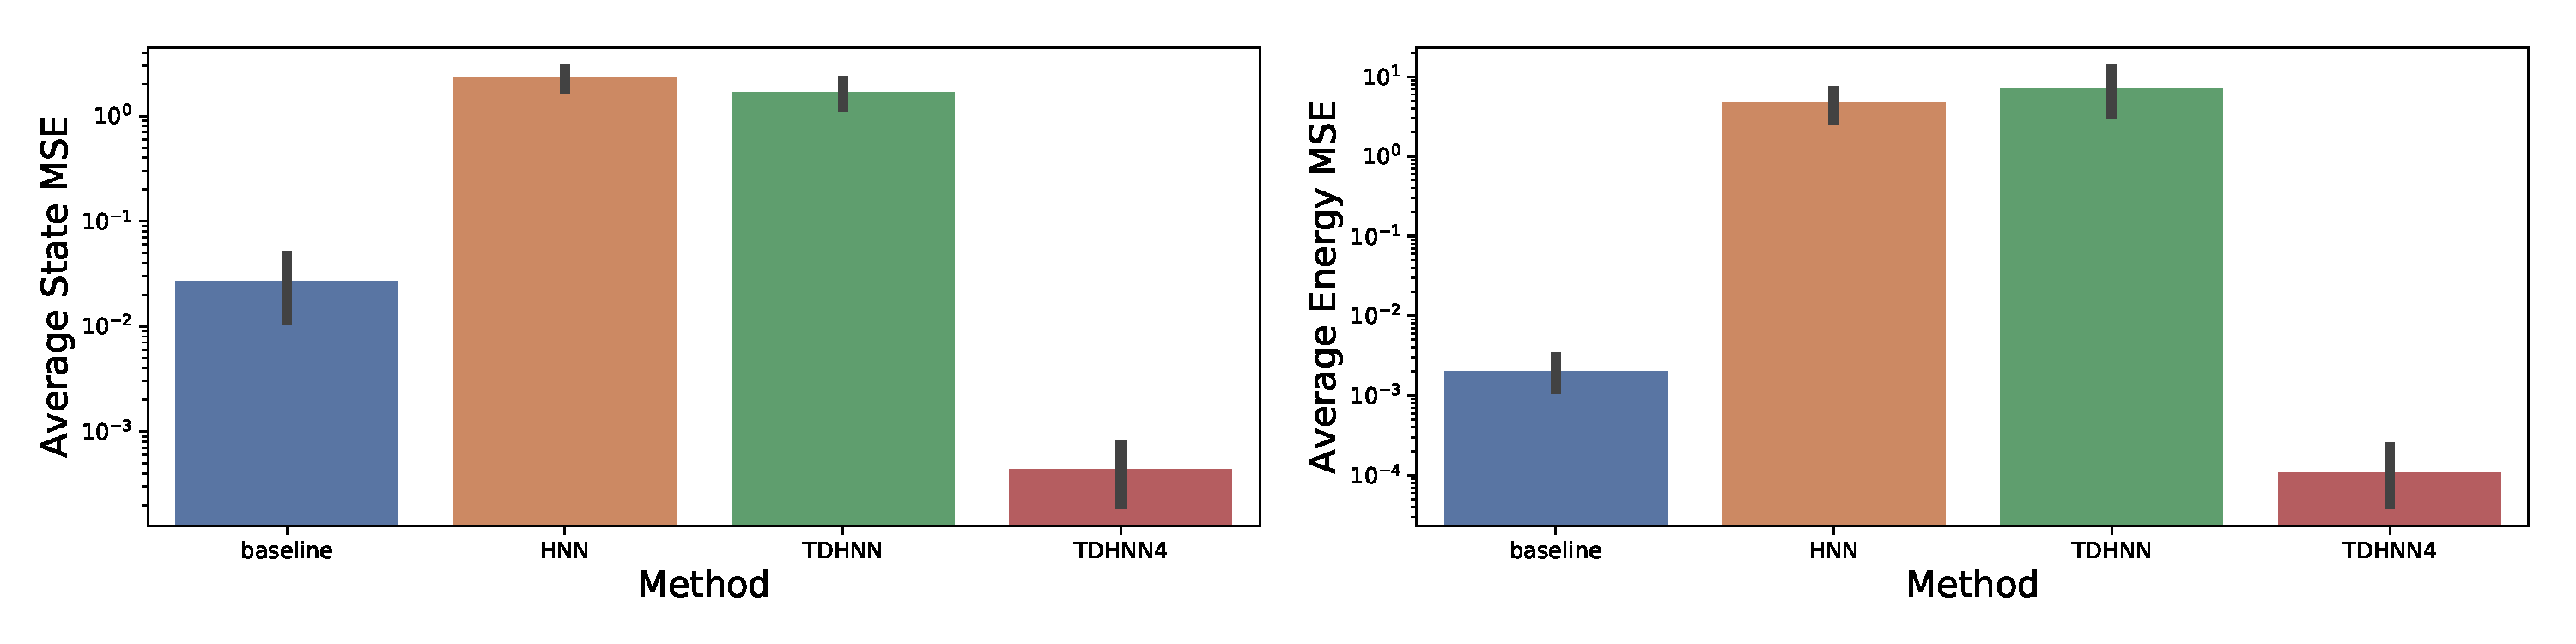
\includegraphics[width=\textwidth]{figures/figures/duffing/1/duffing_errors_0.pdf}
\caption{The average state and energy MSE across 25 test points}
\end{subfigure}
\begin{subfigure}[b]{0.48\textwidth}
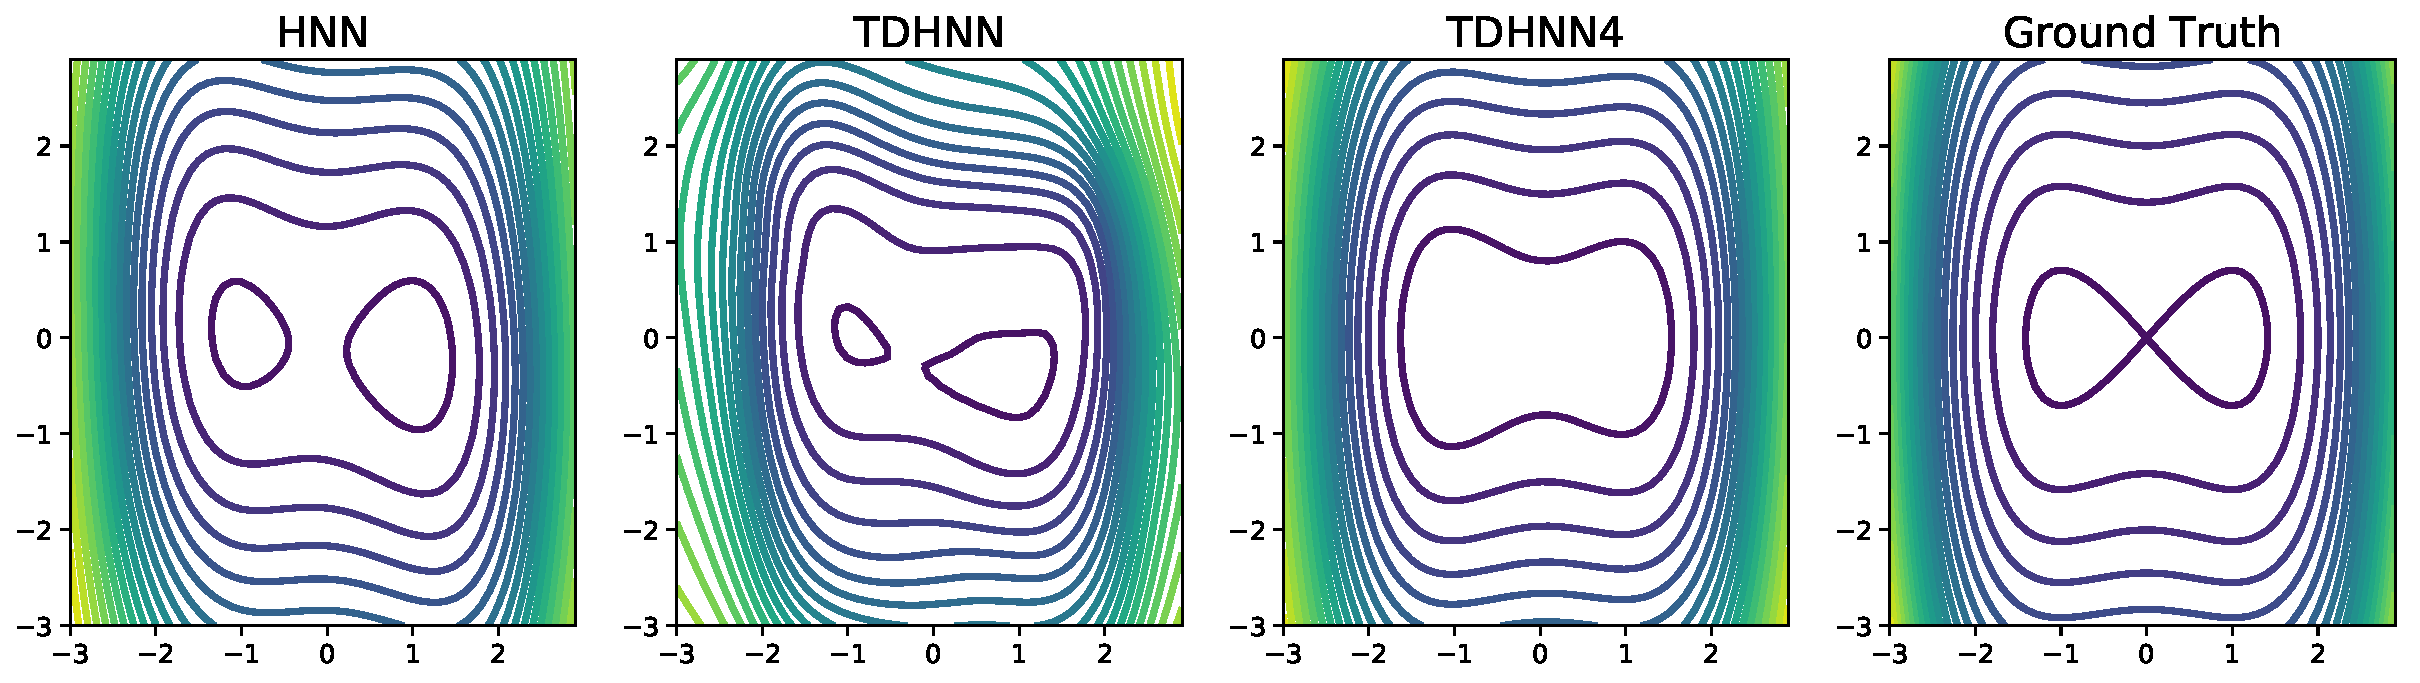
\includegraphics[width=\textwidth]{figures/figures/duffing/1/duffing_hamiltonian_0.pdf}
\caption{The learnt Hamiltonian across methods}
\end{subfigure}
\begin{subfigure}[b]{0.48\textwidth}
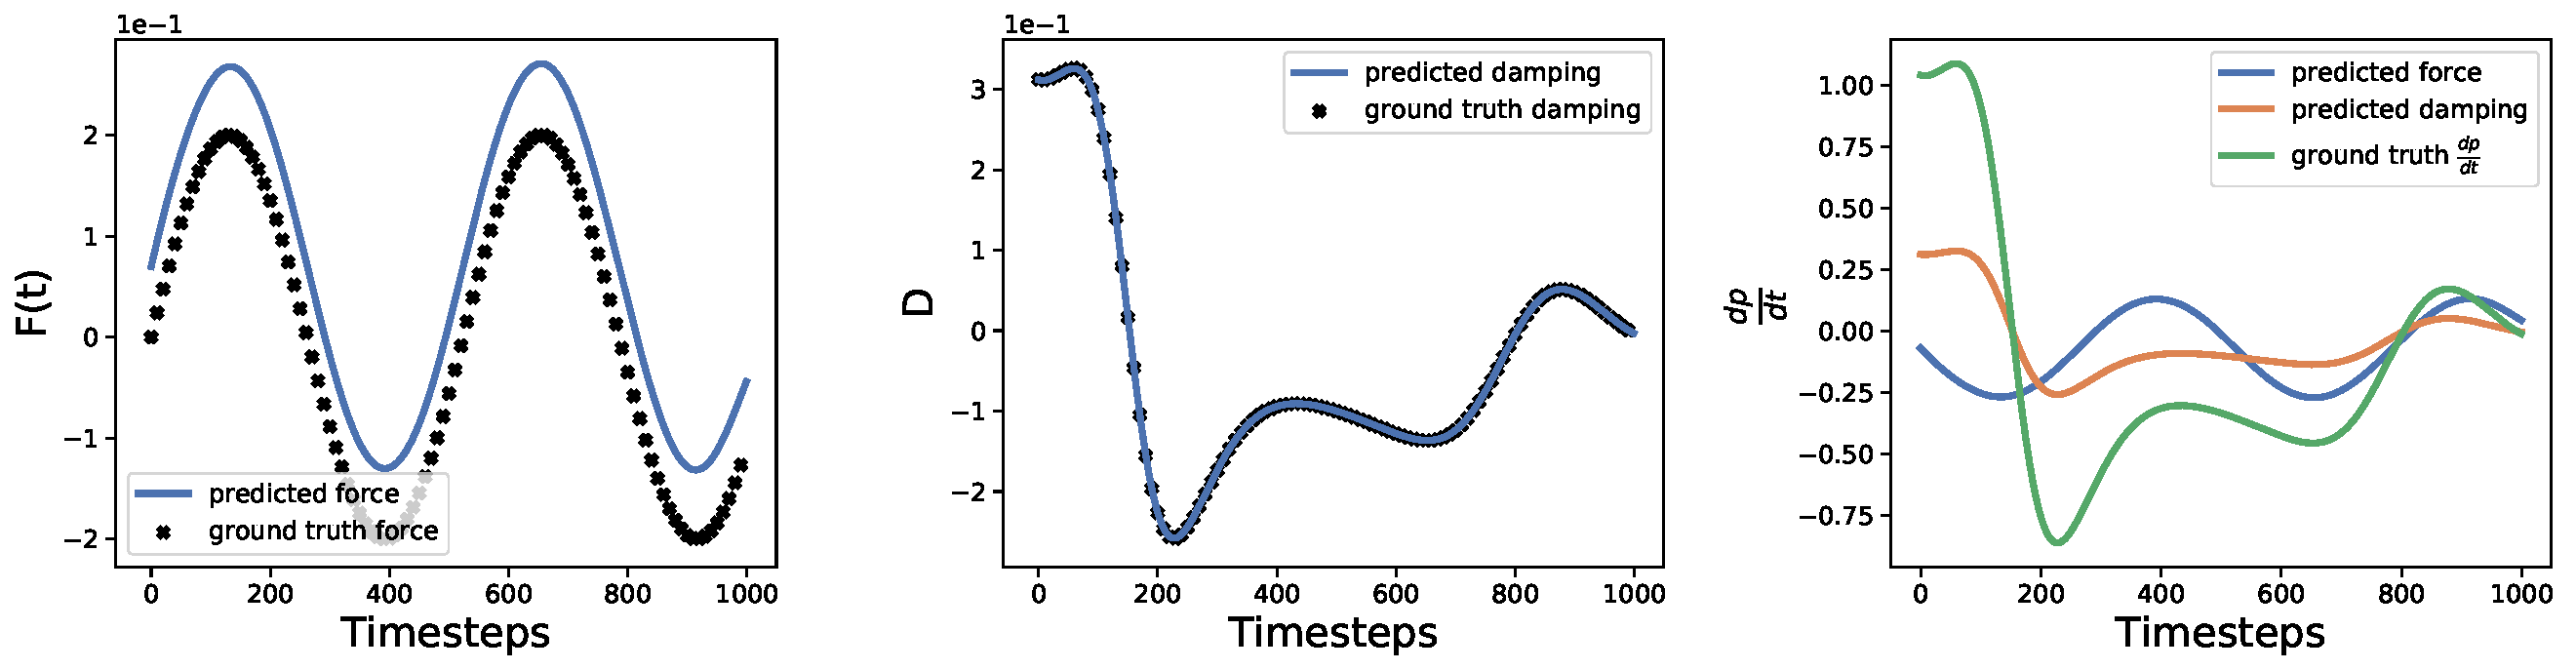
\includegraphics[width=\textwidth]{figures/figures/duffing/1/duffing_dpdt_0.pdf}
\caption{The learnt force and damping of TDHNN4}
\end{subfigure}
\label{duffing_1_full}
\end{figure}
\begin{figure}[!htb]
\centering
\captionsetup{justification=centering}
\begin{subfigure}[b]{0.48\textwidth}
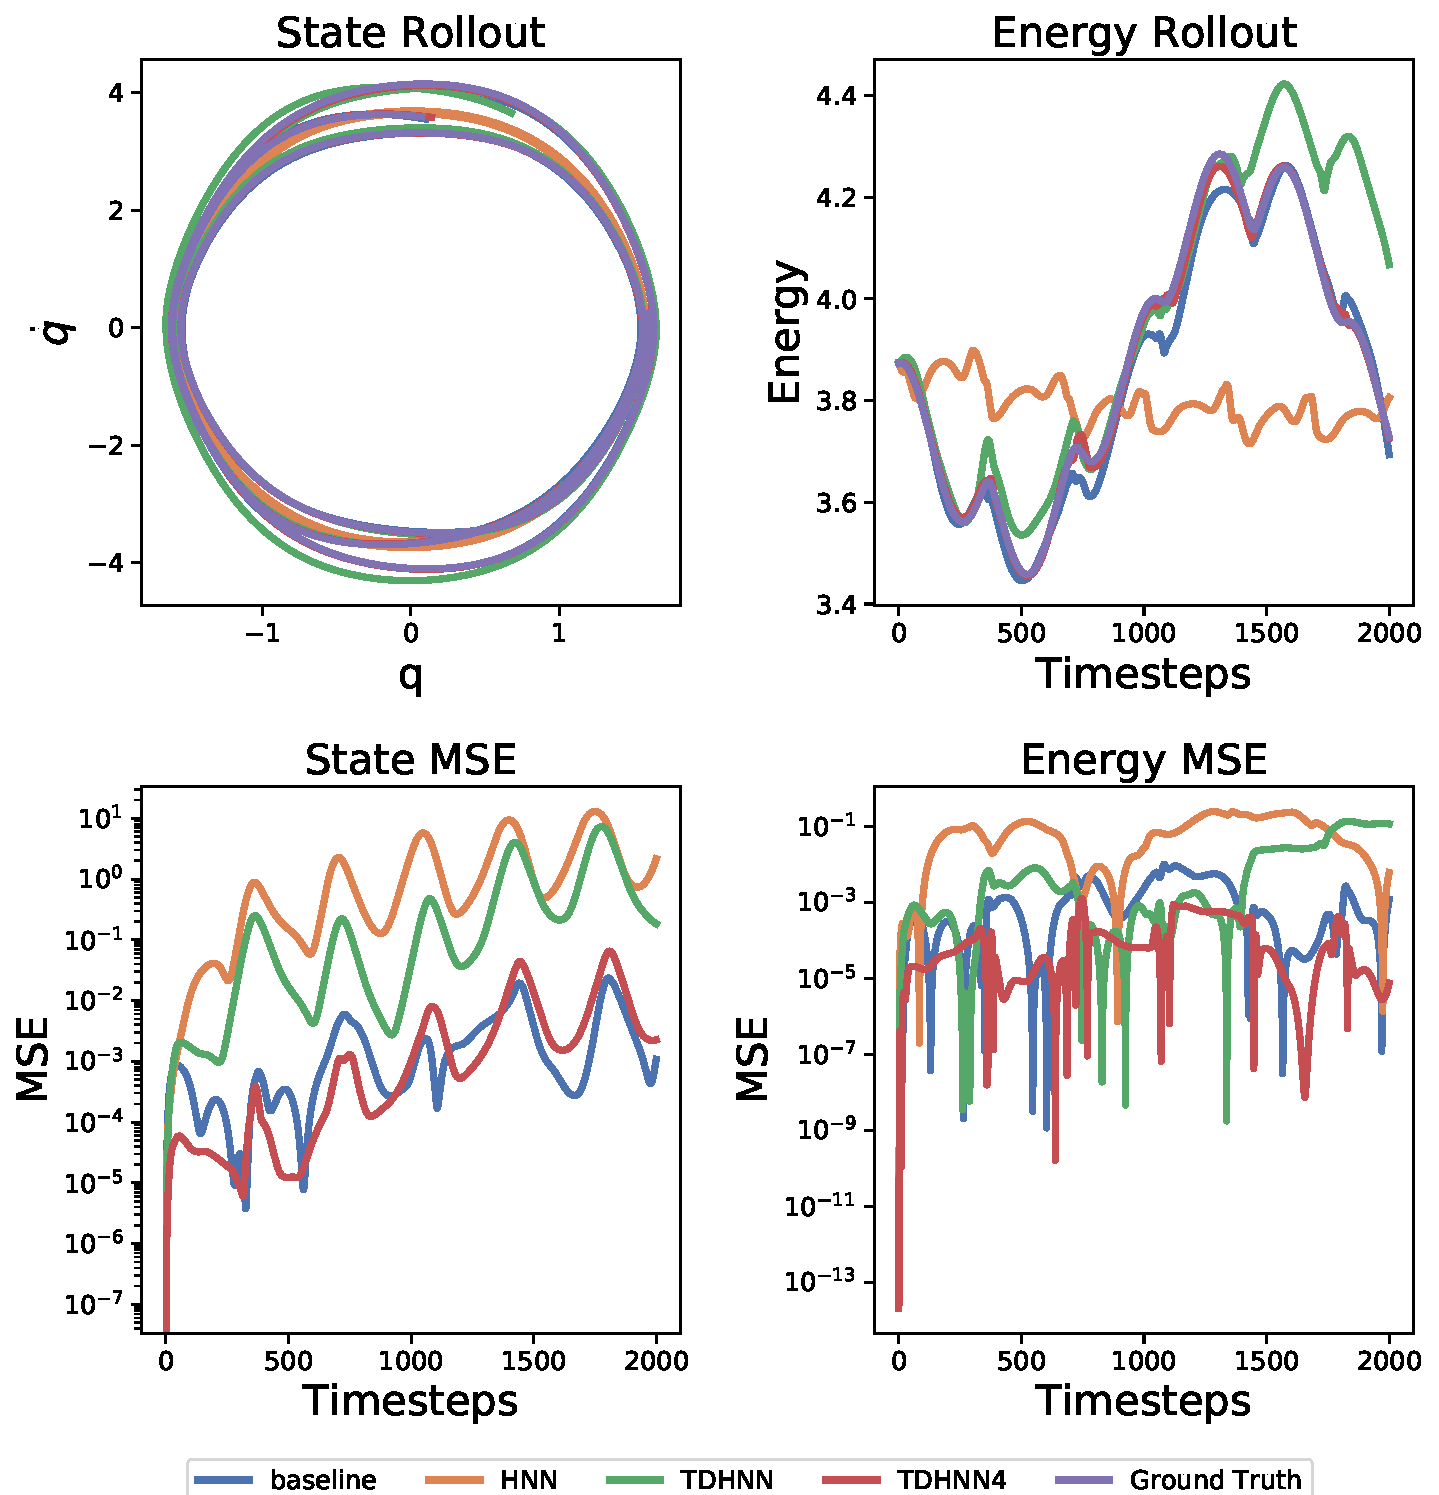
\includegraphics[width=\textwidth]{figures/figures/relativity/1/relativity_long_0.pdf}
\caption{State and energy rollout of an initial condition from the test set}
\end{subfigure}
\begin{subfigure}[b]{0.48\textwidth}
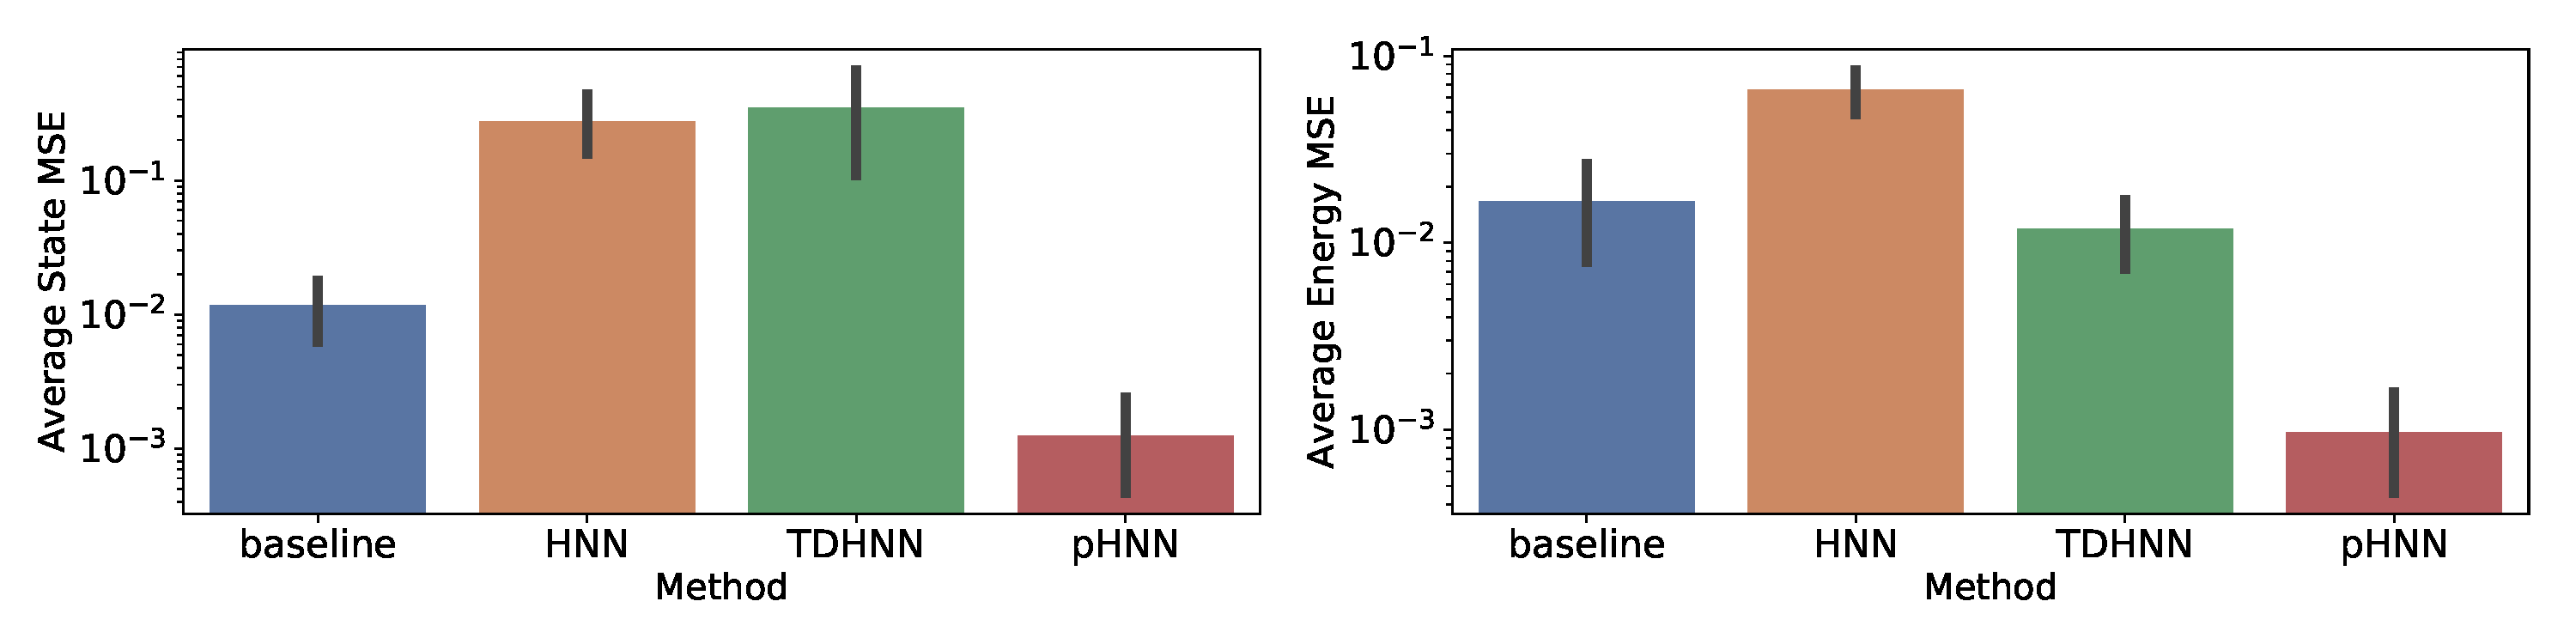
\includegraphics[width=\textwidth]{figures/figures/relativity/1/relativity_errors_0.pdf}
\caption{The average state and energy MSE across 25 test points}
\end{subfigure}
\begin{subfigure}[b]{0.48\textwidth}
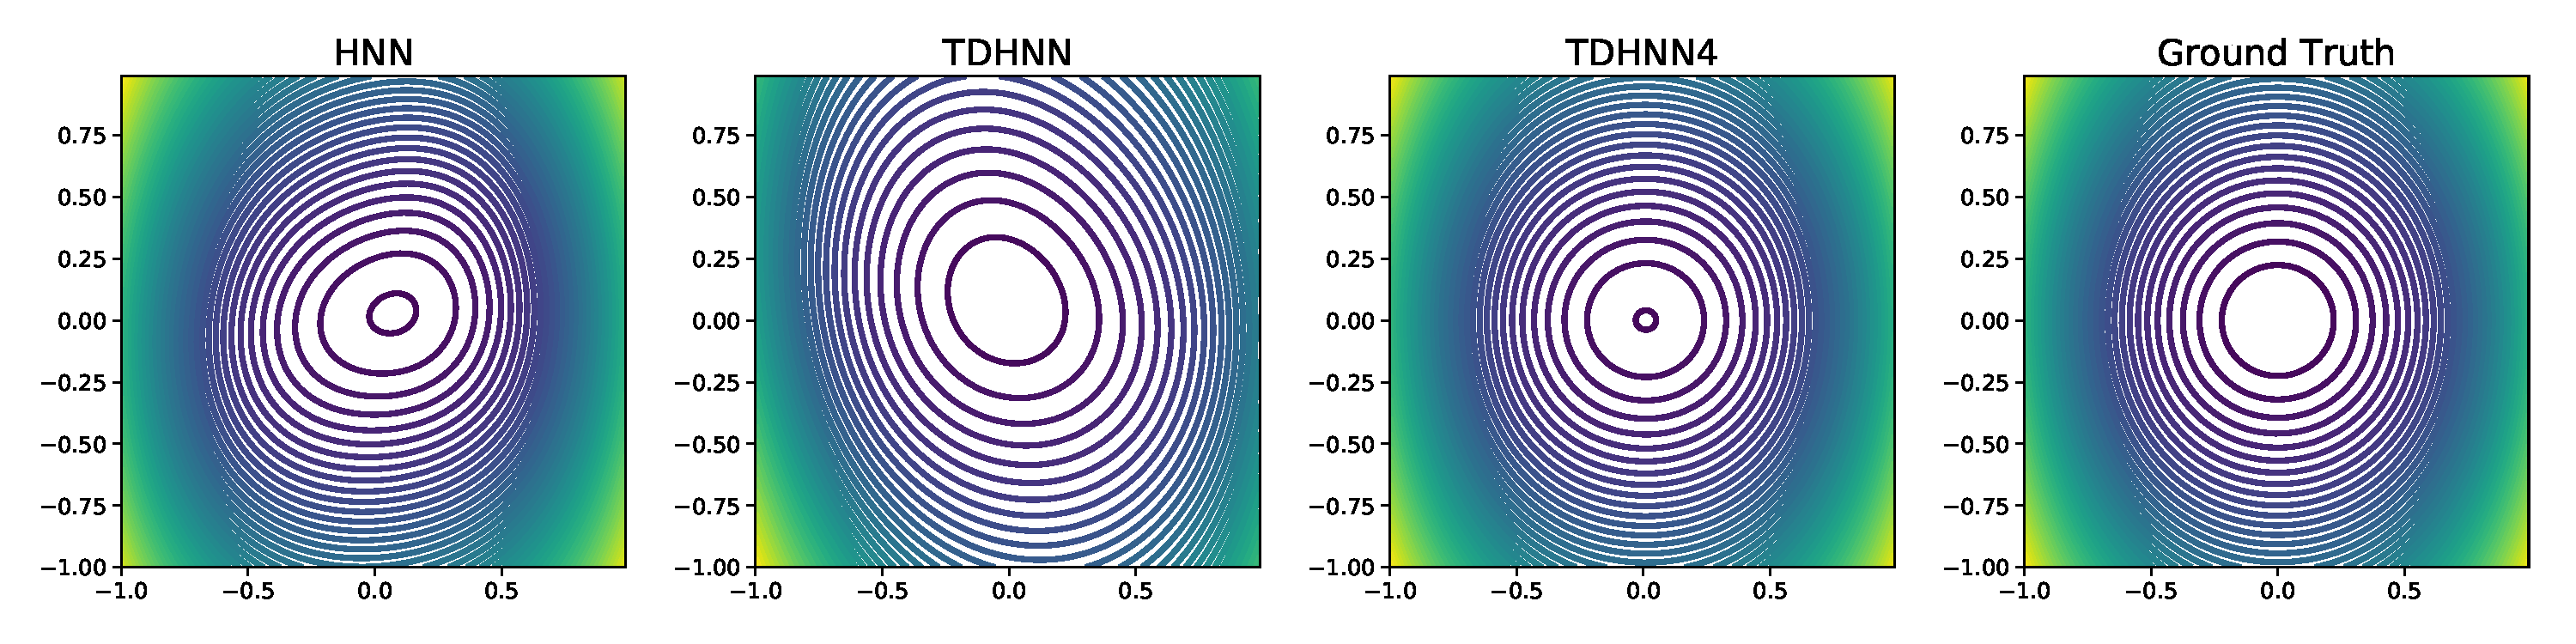
\includegraphics[width=\textwidth]{figures/figures/relativity/1/relativity_ham.pdf}
\caption{The learnt Hamiltonian across methods}
\end{subfigure}
\begin{subfigure}[b]{0.48\textwidth}
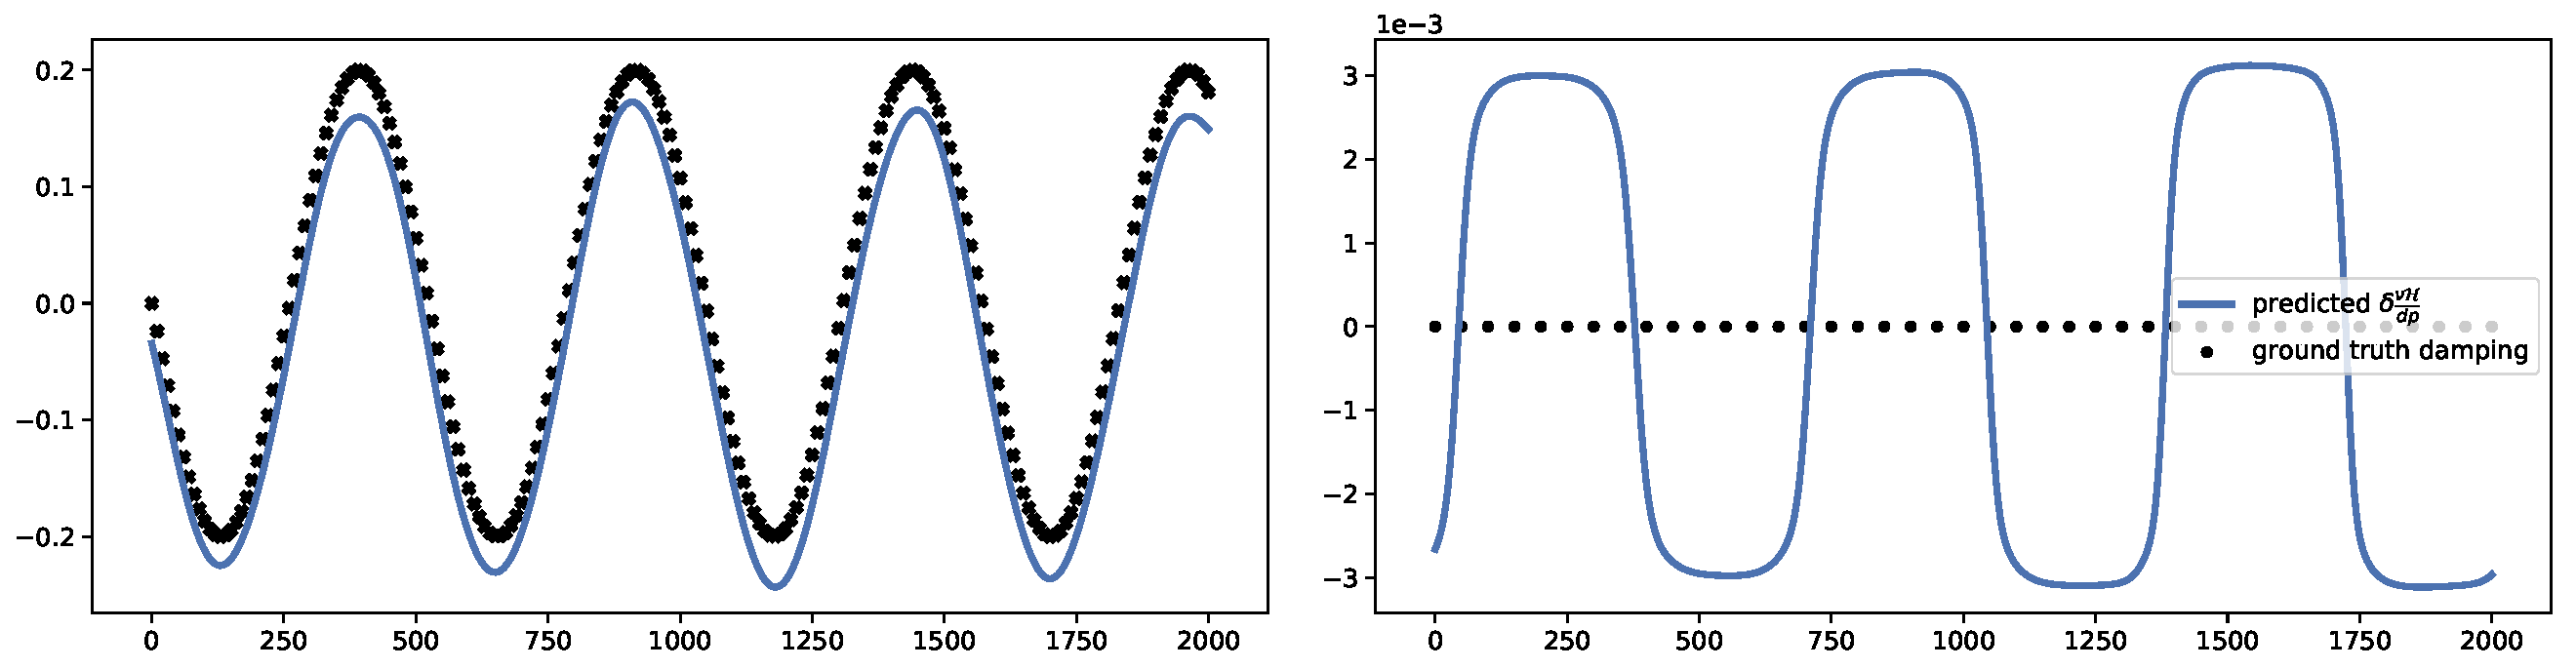
\includegraphics[width=\textwidth]{figures/figures/relativity/1/relativity_dpdt_0.pdf}
\caption{The learnt force and damping of TDHNN4}
\end{subfigure}
\label{duffing_1_full}
\end{figure}

\pagebreak
\onecolumn
\subsection*{C}

During the training of HNN, the authors add gaussian noise with a standard deviation $\sigma=0.1$ to the input state vector data. The reason this is done is to ensure the model is robustly trained. We run a set of experiments to test the robustness to this 'noisy' input. 

\begin{figure}[h!]
\centering
\captionsetup{justification=centering}
\begin{subfigure}[b]{0.42\textwidth}
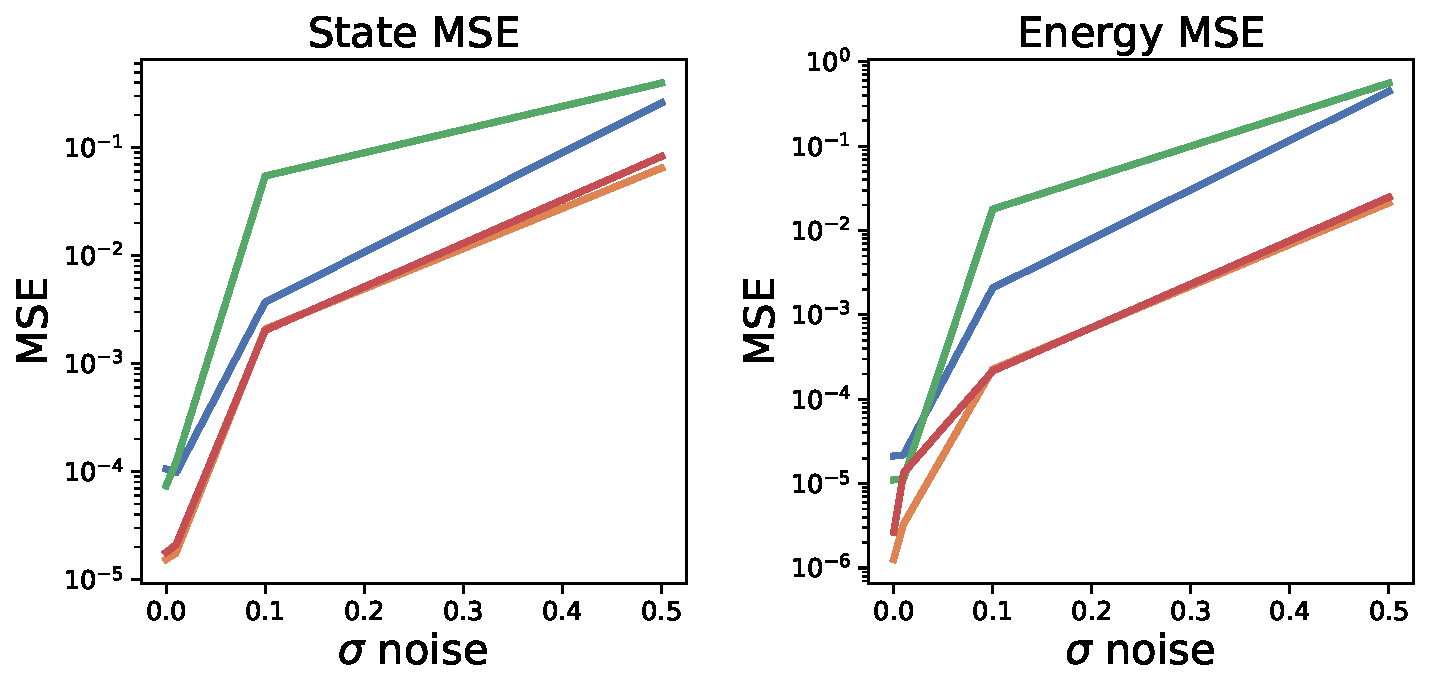
\includegraphics[width=\textwidth]{figures/figures/mass_spring/1/mass_spring_noise_scaling.pdf}
\caption{mass spring}
\end{subfigure}
\begin{subfigure}[b]{0.42\textwidth}
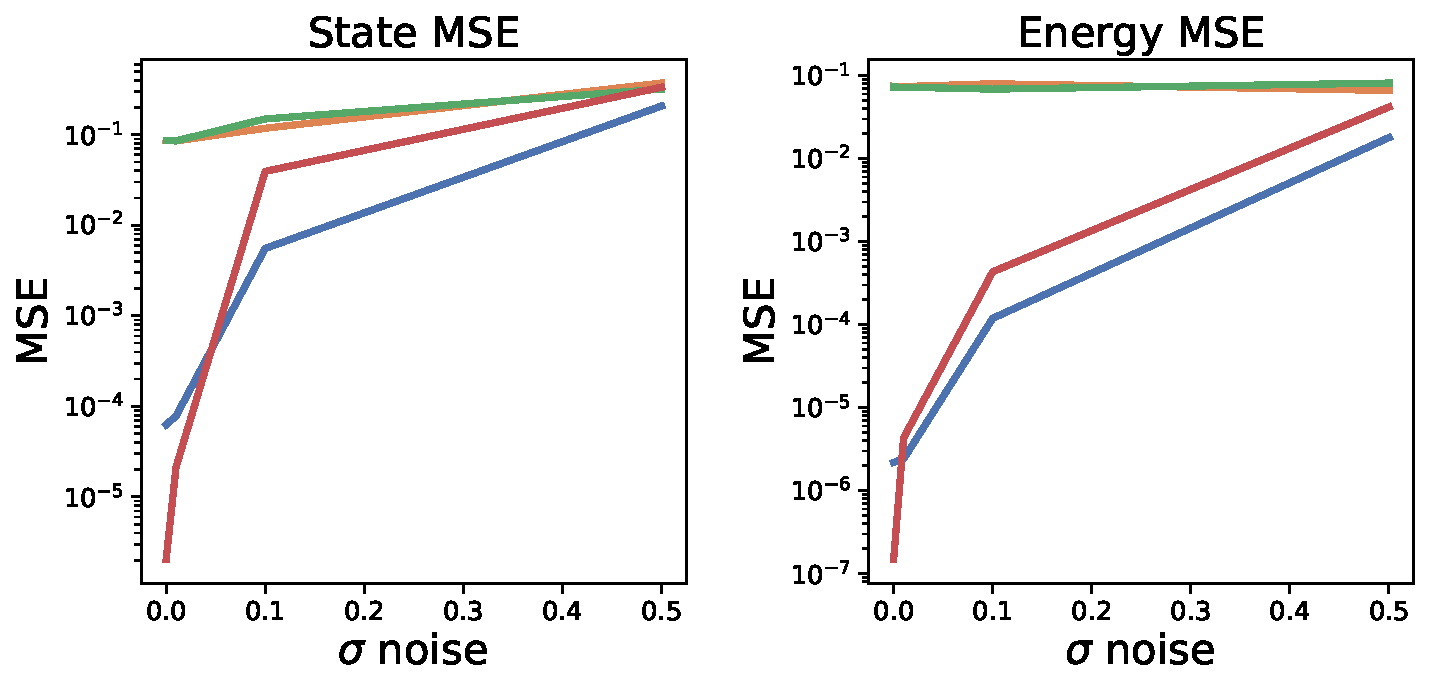
\includegraphics[width=\textwidth]{figures/figures/damped/1/damped_noise_scaling.pdf}
\caption{damped}
\end{subfigure}
\begin{subfigure}[b]{0.42\textwidth}
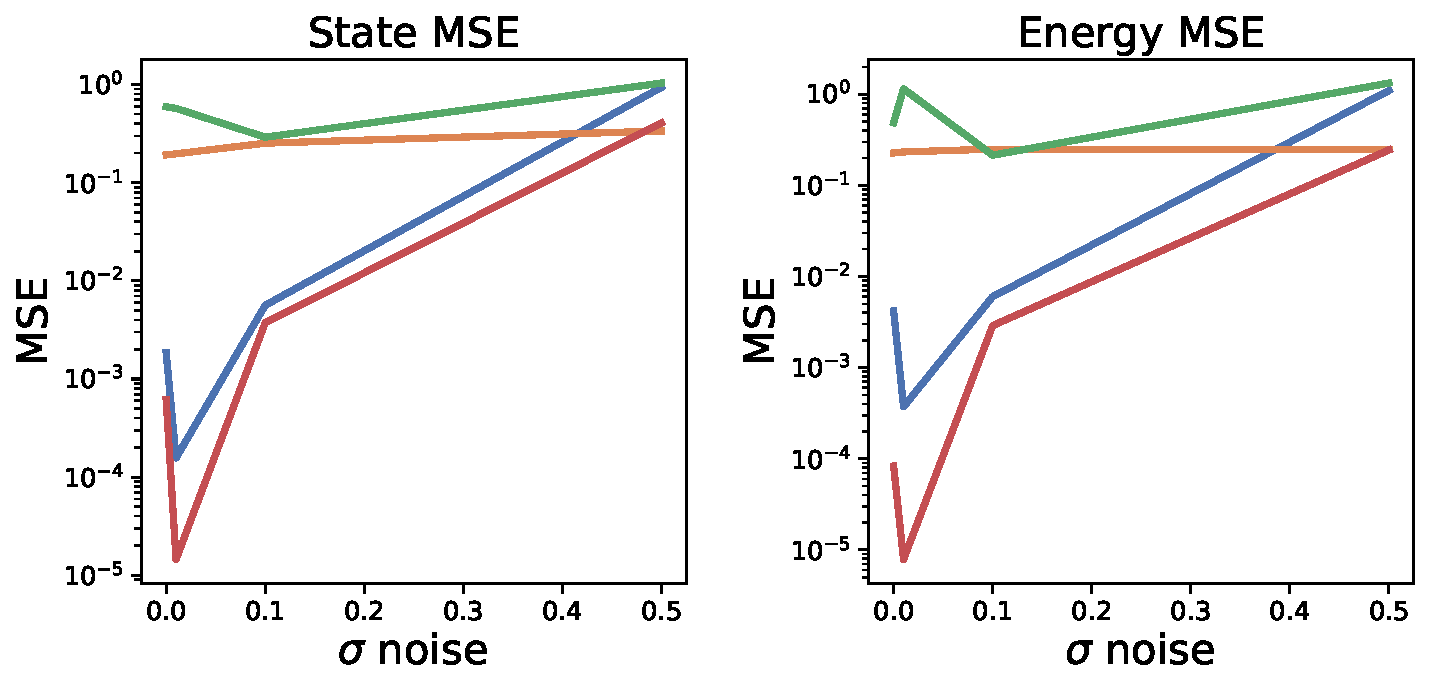
\includegraphics[width=\textwidth]{figures/figures/forced_mass_spring/1/forced_mass_spring_noise_scaling.pdf}
\caption{forced mass spring (I)}
\end{subfigure}
\begin{subfigure}[b]{0.42\textwidth}
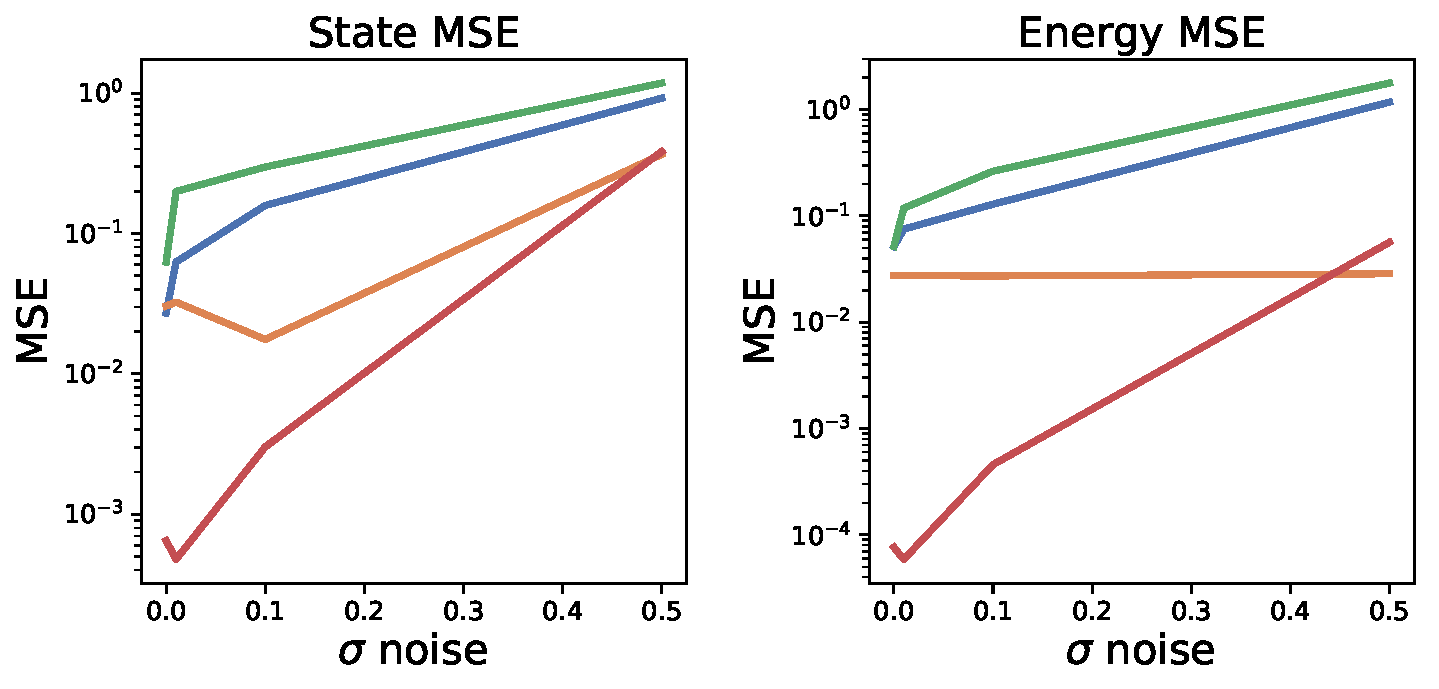
\includegraphics[width=\textwidth]{figures/figures/forced_mass_spring/2/forced_mass_spring_noise_scaling.pdf}
\caption{forced mass spring (II)}
\end{subfigure}
\begin{subfigure}[b]{0.42\textwidth}
\includegraphics[width=\textwidth]{figures/figures/duffing/1/duffing_noise_scaling.pdf}
\caption{duffing}
\end{subfigure}
\begin{subfigure}[b]{0.42\textwidth}
\includegraphics[width=\textwidth]{figures/figures/relativity/1/relativity_noise_scaling.pdf}
\caption{relativity}
\end{subfigure}
\end{figure}

\subsection*{D}

\begin{figure}[h!]
\centering
\includegraphics[width=.8\textwidth]{figures/forceanddampingregulariseroptimisation.pdf}
\caption{Hyperparameter Optimization for TDHNN4. We plot, for each system, the validation loss as a function of the $\alpha$ and $\beta$ parameters from the loss in eqn. 5}
\end{figure}


\end{document}
